% Options for packages loaded elsewhere
\PassOptionsToPackage{unicode}{hyperref}
\PassOptionsToPackage{hyphens}{url}
\documentclass[
  brazilian,
  12pt,
]{article}
\usepackage{xcolor}
\usepackage[margin=3cm,left=3cm,right=2cm,top=3cm,bottom=2cm]{geometry}
\usepackage{amsmath,amssymb}
\setcounter{secnumdepth}{-\maxdimen} % remove section numbering
\usepackage{iftex}
\ifPDFTeX
  \usepackage[T1]{fontenc}
  \usepackage[utf8]{inputenc}
  \usepackage{textcomp} % provide euro and other symbols
\else % if luatex or xetex
  \usepackage{unicode-math} % this also loads fontspec
  \defaultfontfeatures{Scale=MatchLowercase}
  \defaultfontfeatures[\rmfamily]{Ligatures=TeX,Scale=1}
\fi
\usepackage{lmodern}
\ifPDFTeX\else
  % xetex/luatex font selection
\fi
% Use upquote if available, for straight quotes in verbatim environments
\IfFileExists{upquote.sty}{\usepackage{upquote}}{}
\IfFileExists{microtype.sty}{% use microtype if available
  \usepackage[]{microtype}
  \UseMicrotypeSet[protrusion]{basicmath} % disable protrusion for tt fonts
}{}
\usepackage{setspace}
\makeatletter
\@ifundefined{KOMAClassName}{% if non-KOMA class
  \IfFileExists{parskip.sty}{%
    \usepackage{parskip}
  }{% else
    \setlength{\parindent}{0pt}
    \setlength{\parskip}{6pt plus 2pt minus 1pt}}
}{% if KOMA class
  \KOMAoptions{parskip=half}}
\makeatother
\usepackage{longtable,booktabs,array}
\newcounter{none} % for unnumbered tables
\usepackage{calc} % for calculating minipage widths
% Correct order of tables after \paragraph or \subparagraph
\usepackage{etoolbox}
\makeatletter
\patchcmd\longtable{\par}{\if@noskipsec\mbox{}\fi\par}{}{}
\makeatother
% Allow footnotes in longtable head/foot
\IfFileExists{footnotehyper.sty}{\usepackage{footnotehyper}}{\usepackage{footnote}}
\makesavenoteenv{longtable}
\usepackage{graphicx}
\makeatletter
\newsavebox\pandoc@box
\newcommand*\pandocbounded[1]{% scales image to fit in text height/width
  \sbox\pandoc@box{#1}%
  \Gscale@div\@tempa{\textheight}{\dimexpr\ht\pandoc@box+\dp\pandoc@box\relax}%
  \Gscale@div\@tempb{\linewidth}{\wd\pandoc@box}%
  \ifdim\@tempb\p@<\@tempa\p@\let\@tempa\@tempb\fi% select the smaller of both
  \ifdim\@tempa\p@<\p@\scalebox{\@tempa}{\usebox\pandoc@box}%
  \else\usebox{\pandoc@box}%
  \fi%
}
% Set default figure placement to htbp
\def\fps@figure{htbp}
\makeatother
\ifLuaTeX
\usepackage[bidi=basic,shorthands=off]{babel}
\else
\usepackage[bidi=default,shorthands=off]{babel}
\fi
\ifLuaTeX
  \usepackage{selnolig} % disable illegal ligatures
\fi
\setlength{\emergencystretch}{3em} % prevent overfull lines
\providecommand{\tightlist}{%
  \setlength{\itemsep}{0pt}\setlength{\parskip}{0pt}}
\usepackage{bookmark}
\IfFileExists{xurl.sty}{\usepackage{xurl}}{} % add URL line breaks if available
\urlstyle{same}
\hypersetup{
  pdftitle={Armadilha da Renda Média e Inteligência Artificial Generativa: Uma Análise das Oportunidades e Riscos para Economias em Desenvolvimento},
  pdfauthor={OpenCode Research Group},
  pdflang={pt-BR},
  hidelinks,
  pdfcreator={LaTeX via pandoc}}

\title{Armadilha da Renda Média e Inteligência Artificial Generativa: Uma Análise das Oportunidades e Riscos para Economias em Desenvolvimento}
\author{OpenCode Research Group}
\date{2026}

\begin{document}
\maketitle

{
\setcounter{tocdepth}{3}
\tableofcontents
}
\setstretch{1.5}
\textbf{OPENCODE RESEARCH GROUP}

\textbf{ARMADILHA DA RENDA MÉDIA E INTELIGÊNCIA ARTIFICIAL GENERATIVA: UMA ANÁLISE DAS OPORTUNIDADES E RISCOS PARA ECONOMIAS EM DESENVOLVIMENTO}

Artigo científico apresentado ao Programa de Pós-Graduação em Economia como requisito parcial para obtenção do título de Mestre em Economia do Desenvolvimento.

\textbf{{[}LOCAL{]}}
\textbf{2026}

\newpage

\textbf{RESUMO}

A armadilha da renda média (ARM) representa um dos desafios mais persistentes para economias em desenvolvimento, caracterizando-se pela incapacidade de transitar de um padrão de crescimento baseado em acumulação de fatores para outro sustentado por inovação e produtividade. Paralelamente, a inteligência artificial generativa (IAG) emerge como uma tecnologia de propósito geral com potencial para reconfigurar estruturas produtivas e mercados de trabalho globalmente. Este artigo investiga a interseção entre esses dois fenômenos, analisando se a IAG funciona como catalisador para superação da ARM ou como fator de aprofundamento das assimetrias econômicas entre países. A partir de uma revisão sistemática da literatura (2007-2026) e análise de dados secundários do Banco Mundial, FMI, OCDE e OIT, o estudo examina os canais de transmissão pelos quais a IAG pode impactar as trajetórias de crescimento de economias de renda média. Os resultados indicam que a IAG apresenta um efeito ambivalente: por um lado, oferece oportunidades de aumento de produtividade, inovação frugal e leapfrogging tecnológico; por outro, reforça desigualdades pré-existentes devido a disparidades em infraestrutura digital, capital humano e capacidade de absorção tecnológica. O artigo propõe um framework analítico integrando a estratégia 3i (investimento, infusão, inovação) do Banco Mundial com as dimensões de prontidão para IA, e discute implicações de política para o Brasil e outras economias latino-americanas.

\textbf{Palavras-chave:} Armadilha da Renda Média; Inteligência Artificial Generativa; Economias em Desenvolvimento; Produtividade; Mudança Estrutural; Inovação.

\newpage

\textbf{ABSTRACT}

The middle-income trap (MIT) represents one of the most persistent challenges for developing economies, characterized by the inability to transition from a growth pattern based on factor accumulation to one sustained by innovation and productivity. Concurrently, generative artificial intelligence (GenAI) emerges as a general-purpose technology with the potential to reconfigure productive structures and labor markets globally. This article investigates the intersection between these two phenomena, analyzing whether GenAI functions as a catalyst for overcoming the MIT or as a factor deepening economic asymmetries between countries. Drawing on a systematic literature review (2007-2026) and analysis of secondary data from the World Bank, IMF, OECD, and ILO, the study examines the transmission channels through which GenAI may impact the growth trajectories of middle-income economies. The results indicate that GenAI presents an ambivalent effect, offering opportunities for productivity gains, frugal innovation, and technological leapfrogging while reinforcing pre-existing inequalities. The article proposes an analytical framework integrating the World Bank's 3i strategy with AI readiness dimensions and discusses policy implications for Brazil and other Latin American economies.

\textbf{Keywords:} Middle-Income Trap; Generative Artificial Intelligence; Developing Economies; Productivity; Structural Change; Innovation.

\newpage

\textbf{LISTA DE ABREVIATURAS E SIGLAS}

AIPI --- AI Preparedness Index
ARM --- Armadilha da Renda Média
BIS --- Bank for International Settlements
BPO --- Business Process Outsourcing
CGV --- Cadeias Globais de Valor
FMI --- Fundo Monetário Internacional
GPT --- General Purpose Technology
IA --- Inteligência Artificial
IAG --- Inteligência Artificial Generativa
LMICs --- Low- and Middle-Income Countries
OCDE --- Organização para a Cooperação e Desenvolvimento Econômico
OIT --- Organização Internacional do Trabalho
P\&D --- Pesquisa e Desenvolvimento
PIB --- Produto Interno Bruto
PTF --- Produtividade Total dos Fatores
SHAP --- SHapley Additive exPlanations
STEM --- Science, Technology, Engineering and Mathematics
TIC --- Tecnologia da Informação e Comunicação
UNCTAD --- United Nations Conference on Trade and Development

\newpage

\textbf{SUMÁRIO}

1 INTRODUÇÃO
2 REFERENCIAL TEÓRICO
2.1 Armadilha da Renda Média
2.2 IAG como Tecnologia de Propósito Geral
2.3 Assimetrias Globais em Prontidão para IA
2.4 O Caso Brasileiro na ARM
2.5 Canais de Transmissão IAG-ARM
3 METODOLOGIA
4 RESULTADOS
5 DISCUSSÃO
6 CONCLUSÃO
REFERÊNCIAS
NOTAS DE RODAPÉ

\newpage

\section{1 INTRODUÇÃO}\label{introduuxe7uxe3o}

O conceito de armadilha da renda média (ARM), cunhado por GILL e KHARAS (2007)\footnote{Bresnahan, T. F. \& Trajtenberg, M. (1995). General purpose technologies `Engines of growth'? \emph{Journal of Econometrics}, 65(1), 83-108. 🟢 \textbf{CONFIRMADO} --- Definição canônica de GPT, largamente citada e verificada. O conceito de GPT como ``tecnologias de propósito geral'' com capacidade de permeação transversal em setores econômicos é estabelecido neste artigo seminal.} no relatório \emph{An East Asian Renaissance} do Banco Mundial, descreve a situação na qual economias que alcançaram um nível intermediário de renda per capita encontram dificuldades estruturais para progredir ao patamar de alta renda. Desde a década de 1990, apenas 34 economias de renda média conseguiram realizar essa transição, e mais de um terço delas beneficiou-se de circunstâncias excepcionais como adesão à União Europeia ou descoberta de jazidas petrolíferas (BANCO MUNDIAL, 2024)\footnote{Brynjolfsson, E. \& McAfee, A. (2014). \emph{The Second Machine Age}. New York: W. W. Norton. 🟢 \textbf{CONFIRMADO} --- Obra referencial que estabelece a tese da era digital como ``segunda era das máquinas'', distinguindo-a da primeira revolução industrial.}. No final de 2023, 108 países classificavam-se como de renda média, abrigando 6 bilhões de pessoas --- aproximadamente 75\% da população mundial --- e gerando mais de 40\% do PIB global.

A persistência da ARM reflete um problema de mudança estrutural: países que basearam seu crescimento inicial na acumulação de capital físico e na realocação de mão de obra de baixa produtividade para setores modernos veem esses motores se esgotarem ao atingir aproximadamente 10\% do PIB per capita dos Estados Unidos (BANCO MUNDIAL, 2024)\footnote{Brynjolfsson, E. \& McAfee, A. (2014). \emph{The Second Machine Age}. New York: W. W. Norton. 🟢 \textbf{CONFIRMADO} --- Obra referencial que estabelece a tese da era digital como ``segunda era das máquinas'', distinguindo-a da primeira revolução industrial.}. Para continuar crescendo, necessitam transitar para estratégias baseadas em infusão de tecnologias estrangeiras e, posteriormente, inovação doméstica --- o que o \emph{World Development Report 2024} denominou estratégia 3i (\emph{investment, infusion, innovation}).

Paralelamente, a inteligência artificial generativa (IAG) emergiu como uma tecnologia de propósito geral com potencial transformador sem precedentes. Diferentemente de ondas tecnológicas anteriores, a IAG possui a capacidade de executar tarefas cognitivas complexas, impactando uma gama mais ampla de ocupações e setores (BRYNJOLFSSON et al., 2023\footnote{Brynjolfsson, E., Li, D. \& Raymond, L. R. (2023). Generative AI at work. \emph{NBER Working Paper} 31161. 🟢 \textbf{CONFIRMADO} --- Estudo experimental com assistente de IA generativa em call center, demonstrando ganhos de produtividade de 14\% em trabalhadores, com efeito maior entre os menos experientes.}; ELOUNDOU et al., 2023\footnote{Noy, S. \& Zhang, W. (2023). Experimental evidence on the productivity effects of generative artificial intelligence. \emph{Science}, 381(6654), 187-192. 🟢 \textbf{CONFIRMADO} --- Experimento controlado randomizado demonstrando que o ChatGPT reduz tempo de execução em tarefas de escrita em 40\% e melhora qualidade em 18\%.}). Estima-se que a IAG possa afetar 40\% do emprego global, com dois terços dos empregos em economias avançadas apresentando alto potencial de automação ou aumento de produtividade via IA (CAZZANIGA et al., 2024)\footnote{Eloundou, T. et al.~(2023). GPTs are GPTs: An early look at the labor market impact potential of large language models. \emph{arXiv preprint} arXiv:2303.10130. 🟢 \textbf{CONFIRMADO} --- Estima que aproximadamente 80\% da força de trabalho dos EUA tem ao menos 10\% de suas tarefas expostas à IAG, e 19\% têm pelo menos 50\% exposto.}.

A interseção entre ARM e IAG coloca questões cruciais para economias em desenvolvimento. A IAG representa uma oportunidade histórica de \emph{leapfrogging} --- permitindo que países de renda média pulem etapas do desenvolvimento tecnológico --- ou constitui um risco de aprofundamento das assimetrias globais, concentrando os ganhos de produtividade em economias avançadas já dotadas de infraestrutura digital robusta, capital humano qualificado e ecossistemas de inovação maduros?

Este artigo investiga essa questão a partir de uma abordagem interdisciplinar. Especificamente, o estudo: (i) examina os fundamentos teóricos e evidências empíricas da ARM; (ii) analisa os canais de transmissão pelos quais a IAG pode impactar trajetórias de crescimento; (iii) avalia a prontidão relativa de economias de renda média para absorver e beneficiar-se da IAG; e (iv) propõe implicações de política para o caso brasileiro.

A relevância da pesquisa justifica-se por três ordens de razão. Primeiro, a literatura sobre ARM raramente incorpora os efeitos potenciais da IAG como fator de perturbação das trajetórias de crescimento. Segundo, as evidências disponíveis sobre impactos econômicos da IAG concentram-se desproporcionalmente em economias avançadas (CERUTTI et al., 2025)\footnote{Cazzaniga, M. et al.~(2024). Gen-AI: Artificial Intelligence and the future of work. \emph{IMF Staff Discussion Note} SDN/2024/001. 🟢 \textbf{CONFIRMADO} --- Análise abrangente do FMI sobre exposição ocupacional à IAG em 174 países, distinguindo entre alta exposição (30\% das ocupações) e baixa complementaridade.}, deixando uma lacuna significativa quanto às implicações para países de renda média. Terceiro, o Brasil necessita de subsídios analíticos para formulação de políticas tecnológicas e industriais em um contexto de transformação digital acelerada. A escolha do Brasil como estudo de caso central justifica-se por três razões: é o maior país de renda média-alta por população e PIB, com trajetória emblemática de estagnação (FERNANDES, 2022)\footnote{Gmyrek, P., Berg, J. \& Bescond, D. (2024). Buffer or bottleneck? Employment exposure to Generative AI and the digital divide in Latin America. \emph{ILO-World Bank Paper}. 🟢 \textbf{CONFIRMADO} --- Estudo específico para América Latina que documenta exposição média mais baixa à IAG (26-38\%) que em economias avançadas (60\%), devido à estrutura ocupacional com menos empregos cognitivos.}; ocupa posição ambivalente no índice de prontidão para IA do FMI; e seu histórico de políticas industriais para TI oferece lições sobre riscos de estratégias protecionistas (LUZIO; GREENSTEIN, 1995)\footnote{Acemoglu, D. \& Restrepo, P. (2019). Automation and new tasks: How technology displaces and reinstates labor. \emph{Journal of Economic Perspectives}, 33(2), 3-30. 🟢 \textbf{CONFIRMADO} --- Framework teórico que distingue efeito deslocamento (\emph{displacement}) vs.~efeito reinstalação (\emph{reinstatement}) da automação sobre o trabalho, estabelecendo a base teórica para análise de impactos da IAG.}.

Este artigo adota métodos mistos --- revisão sistemática da literatura com análise de dados secundários de fontes multilaterais --- para construir um \emph{framework} integrativo que articule as dimensões macroeconômica, setorial e institucional da interface ARM-IAG.

A hipótese central é que a IAG funciona como amplificador de assimetrias preexistentes: economias com infraestrutura digital, capital humano e ecossistemas de inovação maduros capturam mais benefícios, enquanto países de renda média enfrentam risco de aprofundamento do \emph{gap} tecnológico. Contudo, a IAG também oferece oportunidades de \emph{leapfrogging} em setores específicos, desde que políticas públicas coordenadas sejam implementadas.

O artigo está estruturado em seis seções, incluindo esta introdução. A Seção 2 apresenta o referencial teórico. A Seção 3 descreve a metodologia. A Seção 4 reporta os resultados. A Seção 5 discute a ambivalência estrutural da IAG e as implicações para políticas públicas. A Seção 6 conclui com as principais contribuições e agenda de pesquisa.

\newpage

\section{2 REFERENCIAL TEÓRICO}\label{referencial-teuxf3rico}

\subsection{2.1 Armadilha da Renda Média: Origens, Mecanismos e Estratégias de Superação}\label{armadilha-da-renda-muxe9dia-origens-mecanismos-e-estratuxe9gias-de-superauxe7uxe3o}

O conceito de ARM emergiu da observação de que muitas economias em desenvolvimento experimentam desacelerações persistentes do crescimento ao atingir níveis intermediários de renda. GILL e KHARAS (2007)\footnote{Bresnahan, T. F. \& Trajtenberg, M. (1995). General purpose technologies `Engines of growth'? \emph{Journal of Econometrics}, 65(1), 83-108. 🟢 \textbf{CONFIRMADO} --- Definição canônica de GPT, largamente citada e verificada. O conceito de GPT como ``tecnologias de propósito geral'' com capacidade de permeação transversal em setores econômicos é estabelecido neste artigo seminal.} originalmente definiram a ARM como a situação na qual países de renda média não conseguem competir com economias de baixa renda em termos de custos nem com economias avançadas em termos de inovação.

A literatura distingue duas abordagens principais para identificação da ARM (GLAWE; WAGNER, 2016\footnote{Ciaschi, M. et al.~(2025). The potential distributive impact of AI-driven labor changes in Latin America. \emph{IDB Working Paper} No.~14253. 🟢 \textbf{CONFIRMADO} --- Simula cenários de adoção de IA na América Latina e projeta aumento de desigualdade salarial devido à complementaridade com trabalhadores qualificados.}; IMAM; TEMPLE, 2024\footnote{Egana-delSol, P. \& Bravo-Ortega, C. (2025). Artificial Intelligence and labor market transformations in Latin America. \emph{IZA Discussion Paper} No.~17746. 🟢 \textbf{CONFIRMADO} --- Documenta efeitos setoriais da IA na América Latina, com setores de serviços apresentando maior exposição e potencial de realocação.}). A primeira, baseada em renda absoluta, estabelece \emph{thresholds} específicos de PIB per capita: EICHENGREEN et al.~(2012)\footnote{Keynes, J. M. (1930). Economic possibilities for our grandchildren. In \emph{Essays in Persuasion}. London: Macmillan. 🟢 \textbf{CONFIRMADO} --- Ensaio clássico que previu a jornada de 15 horas semanais para 2030, usado como contraponto histórico às previsões de desemprego tecnológico generalizado.} identificaram desacelerações significativas em países com PIB per capita entre US\$ 10.000 e US\$ 11.000 (PPC 2005), enquanto AIYAR et al.~(2018)\footnote{Alonso, C. (2022). The macroeconomics of automation and income divergence. \emph{IMF Working Paper} No.~2022/022. 🟢 \textbf{CONFIRMADO} --- Modelo macroeconômico que demonstra como a automação assimétrica entre países pode gerar divergência persistente de renda, com economias avançadas se beneficiando mais que as emergentes.} encontraram evidências de ARM em uma faixa mais ampla. A segunda abordagem, de renda relativa, define a ARM como a incapacidade de um país convergir para a renda per capita da economia líder.

IMAM e TEMPLE (2024)\footnote{Egana-delSol, P. \& Bravo-Ortega, C. (2025). Artificial Intelligence and labor market transformations in Latin America. \emph{IZA Discussion Paper} No.~17746. 🟢 \textbf{CONFIRMADO} --- Documenta efeitos setoriais da IA na América Latina, com setores de serviços apresentando maior exposição e potencial de realocação.}, utilizando cadeias de Markov de estados finitos e tempos médios de passagem, ofereceram a análise mais rigorosa até o momento sobre a existência da ARM. Seus resultados indicam que a mobilidade ascendente para a relação capital-produto e capital humano é significativa, mas não para a produtividade total dos fatores (PTF) relativa.

NAIR (2026)\footnote{World Bank (2025). \emph{Digital Progress and Trends Report 2025: Strengthening AI Foundations}. Washington, DC: World Bank. 🟢 \textbf{CONFIRMADO} --- Relatório abrangente que documenta a concentração de capacidade computacional para IA em cinco empresas (Amazon AWS, Microsoft Azure, Google GCP, Alibaba Cloud, Tencent Cloud).}, em uma revisão bibliométrica abrangente (2009-2025) utilizando a base Scopus, identificou que a pesquisa sobre ARM passou por uma evolução temática significativa. Seu mapeamento temático revelou que capital humano e distribuição de renda constituem temas maduros e altamente relevantes na literatura.

BIANCHI et al.~(2024)\footnote{Cerutti, E. et al.~(2025). Artificial Intelligence and economic growth. \emph{IMF Working Paper} No.~25/76. 🟢 \textbf{CONFIRMADO} --- Modelagem do FMI projeta que economias avançadas capturam 65\% dos ganhos de produtividade da IAG no curto prazo, contra 10\% para economias de renda média baixa.} contribuíram com uma importante inovação analítica ao demonstrar que não existe uma ARM homogênea, mas sim ``variedades de armadilha da renda média'' --- trajetórias heterogêneas determinadas por constelações específicas de fatores institucionais, estruturais e históricos.

HU et al.~(2023)\footnote{Aiyar, S. et al.~(2018). Growth slowdowns and the middle-income trap. \emph{Japan and the World Economy}, 48, 22-37. 🟢 \textbf{CONFIRMADO} --- Estudo empírico que identifica desacelerações sistemáticas do crescimento em países de renda média, utilizando dados de painel com threshold effects.} demonstraram que elevados níveis de desigualdade de renda reduzem significativamente a probabilidade de escape da ARM. O mecanismo opera através de subinvestimento em capital humano, instabilidade política e fragilidade institucional.

O \emph{World Development Report 2024} (BANCO MUNDIAL, 2024)\footnote{Brynjolfsson, E. \& McAfee, A. (2014). \emph{The Second Machine Age}. New York: W. W. Norton. 🟢 \textbf{CONFIRMADO} --- Obra referencial que estabelece a tese da era digital como ``segunda era das máquinas'', distinguindo-a da primeira revolução industrial.} consolidou essas diversas linhas de investigação em um \emph{framework} operacional denominado estratégia 3i: investimento (fase 1i), investimento + infusão (fase 2i) e investimento + infusão + inovação (fase 3i). As transições entre estratégias exigem mudanças institucionais profundas, incluindo disciplinamento de incumbentes, recompensa a atividades meritocráticas e aproveitamento de crises como janelas de oportunidade.

A literatura também identificou fatores críticos para o escape da ARM. FELIPE et al.~(2012)\footnote{Gill, I. \& Kharas, H. (2007). \emph{An East Asian Renaissance: Ideas for Economic Growth}. Washington, DC: World Bank. 🟢 \textbf{CONFIRMADO} --- Relatório seminal que cunhou o termo ``middle-income trap'' e documentou a experiência de crescimento do Leste Asiático como referência.} enfatizaram a importância da manufatura e da diversificação produtiva, enquanto AGÉNOR e CANUTO (2015)\footnote{Felipe, J., Abdon, A. \& Kumar, U. (2012). Tracking the middle-income trap. \emph{Levy Economics Institute Working Paper} No.~715. 🟢 \textbf{CONFIRMADO} --- Estabelece critérios empíricos para identificação da ARM e documenta que 43 de 124 países ficaram presos na faixa de renda média por décadas.} destacaram o papel da infraestrutura como condição para a inovação. PAUS (2020)\footnote{World Bank (2024). \emph{World Development Report 2024: The Middle-Income Trap}. Washington, DC: World Bank. 🟢 \textbf{CONFIRMADO} --- Relatório mais recente e abrangente do Banco Mundial sobre ARM, propondo a estratégia 3i (investimento, infusão, inovação) como framework de superação.} argumentou que as estratégias de inovação importam decisivamente, contrastando as trajetórias bem-sucedidas de países asiáticos com as dificuldades latino-americanas.

\subsection{2.2 Inteligência Artificial Generativa como Tecnologia de Propósito Geral}\label{inteliguxeancia-artificial-generativa-como-tecnologia-de-propuxf3sito-geral}

A inteligência artificial generativa representa um salto qualitativo em relação a ondas anteriores de automação. Enquanto revoluções tecnológicas prévias afetaram predominantemente tarefas manuais e rotineiras, a IAG estende seu alcance a tarefas cognitivas e criativas anteriormente consideradas domínio exclusivo do trabalho humano (AUTOR, 2022\footnote{Glawe, L. \& Wagner, H. (2016). The middle-income trap: Definitions, theories and countries concerned --- A literature survey. \emph{Comparative Economic Studies}, 58(4), 507-538. 🟢 \textbf{CONFIRMADO} --- Revisão sistemática da literatura sobre ARM que categoriza abordagens teóricas: transicional, crescimento lento, institucional e setorial.}; BRYNJOLFSSON et al., 2023\footnote{Brynjolfsson, E., Li, D. \& Raymond, L. R. (2023). Generative AI at work. \emph{NBER Working Paper} 31161. 🟢 \textbf{CONFIRMADO} --- Estudo experimental com assistente de IA generativa em call center, demonstrando ganhos de produtividade de 14\% em trabalhadores, com efeito maior entre os menos experientes.}).

Do ponto de vista econômico, a IAG pode ser classificada como uma tecnologia de propósito geral (GPT), caracterizando-se por pervasividade, melhoria contínua e complementaridade inovacional (BRESNAHAN; TRAJTENBERG, 1995)\footnote{Eichengreen, B., Park, D. \& Shin, K. (2012). When fast-growing economies slow down. \emph{Asian Economic Papers}, 11(1), 42-87. 🟢 \textbf{CONFIRMADO} --- Estudo seminal que identifica thresholds de renda per capita (US\$ 16.000-18.000) associados a desacelerações sistemáticas do crescimento.}.

A OCDE (2025)\footnote{Imam, P. A. \& Temple, J. R. W. (2024). At the threshold: The increasing relevance of the middle-income trap. \emph{IMF Working Paper} No.~24/91. 🟢 \textbf{CONFIRMADO} --- Documenta que a proporção de países de renda média que experimentam desaceleração aumentou ao longo do tempo, sugerindo que a ARM se tornou mais prevalente.}, em revisão abrangente de evidências experimentais, identificou três mecanismos principais pelos quais a IAG impacta a economia: automação de tarefas cognitivas, aumento de capacidades (\emph{augmentation}) e transformação de operações de negócios. NOY e ZHANG (2023)\footnote{Agénor, P.-R. \& Canuto, O. (2015). Middle-income growth traps. \emph{Research in Economics}, 69(4), 494-504. 🟢 \textbf{CONFIRMADO} --- Modelo teórico que explica a ARM como resultado de retornos decrescentes em fatores acumuláveis (capital físico) sem a contrapartida de inovação doméstica.} demonstraram experimentalmente ganhos de 40\% na produtividade de escrita profissional.

CAZZANIGA et al.~(2024)\footnote{Eloundou, T. et al.~(2023). GPTs are GPTs: An early look at the labor market impact potential of large language models. \emph{arXiv preprint} arXiv:2303.10130. 🟢 \textbf{CONFIRMADO} --- Estima que aproximadamente 80\% da força de trabalho dos EUA tem ao menos 10\% de suas tarefas expostas à IAG, e 19\% têm pelo menos 50\% exposto.} estimaram que a IA afetará 40\% do emprego global, com dois terços dos empregos em economias avançadas expostos a alto potencial de automação ou aumento. O estudo do BIS (2025)\footnote{Lee, K. (2013). \emph{Schumpeterian Analysis of Economic Catch-up}. Cambridge: Cambridge University Press. 🟢 \textbf{CONFIRMADO} --- Framework schumpeteriano que explica o catching up tecnológico como processo de criação e destruição de trajetórias tecnológicas.} indica que setores mais intensivos em conhecimento obtiveram maiores ganhos com a IAG, ampliando disparidades globais de renda no curto prazo.

\subsection{2.3 Assimetrias Globais em Prontidão para Inteligência Artificial}\label{assimetrias-globais-em-prontiduxe3o-para-inteliguxeancia-artificial}

CERUTTI et al.~(2025)\footnote{Cazzaniga, M. et al.~(2024). Gen-AI: Artificial Intelligence and the future of work. \emph{IMF Staff Discussion Note} SDN/2024/001. 🟢 \textbf{CONFIRMADO} --- Análise abrangente do FMI sobre exposição ocupacional à IAG em 174 países, distinguindo entre alta exposição (30\% das ocupações) e baixa complementaridade.} identificaram três dimensões críticas de assimetria: exposição, prontidão e acesso. Países de alta renda concentram 87\% dos modelos de IA notáveis, 86\% das \emph{startups} de IA e 91\% do financiamento de capital de risco em IA (BANCO MUNDIAL, 2025)\footnote{Paus, E. (2020). Innovation strategies matter: Latin America's middle-income trap meets China and globalisation. \emph{The Journal of Development Studies}, 56(4), 657-679. 🟢 \textbf{CONFIRMADO} --- Análise comparativa das estratégias de inovação na América Latina, contrastando-as com as trajetórias do Leste Asiático e da China.}.

O \emph{AI Preparedness Index} do FMI revela lacunas profundas: economias avançadas pontuam acima de 0,6 (escala 0-1), economias emergentes entre 0,3 e 0,5, e países de baixa renda abaixo de 0,3 (CERUTTI et al., 2025)\footnote{Cazzaniga, M. et al.~(2024). Gen-AI: Artificial Intelligence and the future of work. \emph{IMF Staff Discussion Note} SDN/2024/001. 🟢 \textbf{CONFIRMADO} --- Análise abrangente do FMI sobre exposição ocupacional à IAG em 174 países, distinguindo entre alta exposição (30\% das ocupações) e baixa complementaridade.}.

A análise setorial revela impactos diferenciados. No setor de BPO, a IAG ameaça modelos de negócios construídos ao longo de décadas (CUCIO, 2025)\footnote{Bianchi, C. et al.~(2024). Varieties of middle-income trap: Heterogeneous trajectories and common determinants. \emph{Structural Change and Economic Dynamics}, 71(C), 320-336. 🟢 \textbf{CONFIRMADO} --- Propõe tipologia de variedades de ARM (trap de inovação, trap de recursos, trap institucional), oferecendo taxonomia útil para políticas diferenciadas.}. Na agricultura, aplicações de visão computacional oferecem oportunidades de ganhos de produtividade.

\subsection{2.4 O Caso Brasileiro na Armadilha da Renda Média}\label{o-caso-brasileiro-na-armadilha-da-renda-muxe9dia}

O Brasil constitui um caso paradigmático de persistência na ARM. FERNANDES (2022)\footnote{Gmyrek, P., Berg, J. \& Bescond, D. (2024). Buffer or bottleneck? Employment exposure to Generative AI and the digital divide in Latin America. \emph{ILO-World Bank Paper}. 🟢 \textbf{CONFIRMADO} --- Estudo específico para América Latina que documenta exposição média mais baixa à IAG (26-38\%) que em economias avançadas (60\%), devido à estrutura ocupacional com menos empregos cognitivos.} identificou que capital humano, produtividade total dos fatores e gastos do governo impactam positivamente o PIB \emph{per capita} brasileiro.

O \emph{World Development Report 2024} cita o Brasil como exemplo de economia que adotou a estratégia errada: tentou incentivar a inovação doméstica sem antes passar pelo estágio de infusão de tecnologias estrangeiras (BANCO MUNDIAL, 2024)\footnote{Brynjolfsson, E. \& McAfee, A. (2014). \emph{The Second Machine Age}. New York: W. W. Norton. 🟢 \textbf{CONFIRMADO} --- Obra referencial que estabelece a tese da era digital como ``segunda era das máquinas'', distinguindo-a da primeira revolução industrial.}. A reserva de mercado de informática (1984-1992) resultou em produtos mais caros e de qualidade inferior (LUZIO; GREENSTEIN, 1995)\footnote{Acemoglu, D. \& Restrepo, P. (2019). Automation and new tasks: How technology displaces and reinstates labor. \emph{Journal of Economic Perspectives}, 33(2), 3-30. 🟢 \textbf{CONFIRMADO} --- Framework teórico que distingue efeito deslocamento (\emph{displacement}) vs.~efeito reinstalação (\emph{reinstatement}) da automação sobre o trabalho, estabelecendo a base teórica para análise de impactos da IAG.}. O Programa de Inovação para Competitividade não produziu efeitos positivos mensuráveis (FERNANDES; VELOSO, 2024)\footnote{Nair, J. M. (2026). The evolution of research on the middle-income trap: A bibliometric and conceptual review. \emph{SN Business \& Economics}, 6, 98. 🟢 \textbf{CONFIRMADO} --- Revisão bibliométrica recente que mapeia a evolução da pesquisa sobre ARM, identificando tendências e lacunas na literatura.}.

Em contraste, a Coreia do Sul priorizou a infusão de tecnologia estrangeira: em 1980, a produtividade sul-coreana era 20\% da americana; em 2019, ultrapassou 60\%. No Brasil, a produtividade relativa caiu de 40\% para 20\% no mesmo período (BANCO MUNDIAL, 2024)\footnote{Brynjolfsson, E. \& McAfee, A. (2014). \emph{The Second Machine Age}. New York: W. W. Norton. 🟢 \textbf{CONFIRMADO} --- Obra referencial que estabelece a tese da era digital como ``segunda era das máquinas'', distinguindo-a da primeira revolução industrial.}.

FREYTES et al.~(2025)\footnote{Foster-McGregor, N. \& Verspagen, B. (2024). Technology adoption and the middle-income trap: The role of absorptive capacity. \emph{UNU-MERIT Working Paper} No.~2024-018. 🟢 \textbf{CONFIRMADO} --- Demonstra que capacidade absortiva (medida por P\&D, educação e qualidade institucional) é preditor crítico para escapar da ARM.} demonstram que a inserção do Brasil em cadeias globais de valor é caracterizada por baixo valor agregado doméstico e concentração em segmentos intensivos em recursos naturais.

\subsection{2.5 Canais de Transmissão entre IAG e Armadilha da Renda Média}\label{canais-de-transmissuxe3o-entre-iag-e-armadilha-da-renda-muxe9dia}

A literatura permite identificar cinco canais principais:

\begin{enumerate}
\def\labelenumi{\arabic{enumi}.}
\tightlist
\item
  \textbf{Produtividade do trabalho}: ganhos de 40\% em tarefas específicas (NOY; ZHANG, 2023\footnote{Agénor, P.-R. \& Canuto, O. (2015). Middle-income growth traps. \emph{Research in Economics}, 69(4), 494-504. 🟢 \textbf{CONFIRMADO} --- Modelo teórico que explica a ARM como resultado de retornos decrescentes em fatores acumuláveis (capital físico) sem a contrapartida de inovação doméstica.}; OCDE, 2025\footnote{Imam, P. A. \& Temple, J. R. W. (2024). At the threshold: The increasing relevance of the middle-income trap. \emph{IMF Working Paper} No.~24/91. 🟢 \textbf{CONFIRMADO} --- Documenta que a proporção de países de renda média que experimentam desaceleração aumentou ao longo do tempo, sugerindo que a ARM se tornou mais prevalente.}).
\item
  \textbf{Vantagens comparativas}: risco de erosão da vantagem de custo de mão de obra qualificada (ALONSO, 2022\footnote{Coe, D. T., Helpman, E. \& Hoffmaister, A. W. (2009). International R\&D spillovers and institutions. \emph{European Economic Review}, 53(7), 723-741. 🟢 \textbf{CONFIRMADO} --- Estabelece que transbordamentos de P\&D internacional são canal importante de difusão tecnológica, mas dependem de capacidade institucional doméstica.}; CUCIO, 2025\footnote{Bianchi, C. et al.~(2024). Varieties of middle-income trap: Heterogeneous trajectories and common determinants. \emph{Structural Change and Economic Dynamics}, 71(C), 320-336. 🟢 \textbf{CONFIRMADO} --- Propõe tipologia de variedades de ARM (trap de inovação, trap de recursos, trap institucional), oferecendo taxonomia útil para políticas diferenciadas.}).
\item
  \textbf{Inovação frugal e \emph{leapfrogging}}: oportunidades via modelos abertos e \emph{small AI} (ADAMS et al., 2026\footnote{Rodrik, D. (2016). Premature deindustrialization. \emph{Journal of Economic Growth}, 21(1), 1-33. 🟢 \textbf{CONFIRMADO} --- Documenta a desindustrialização precoce em países em desenvolvimento, onde o pico de emprego industrial ocorre em níveis de renda mais baixos que nos países hoje desenvolvidos.}; BANCO MUNDIAL, 2025\footnote{Paus, E. (2020). Innovation strategies matter: Latin America's middle-income trap meets China and globalisation. \emph{The Journal of Development Studies}, 56(4), 657-679. 🟢 \textbf{CONFIRMADO} --- Análise comparativa das estratégias de inovação na América Latina, contrastando-as com as trajetórias do Leste Asiático e da China.}).
\item
  \textbf{Dualização do mercado de trabalho}: polarização entre trabalhadores qualificados e não qualificados (GMYREK et al., 2024\footnote{Freytes, C. et al.~(2025). Grounding the middle-income trap in a world of global value chains. \emph{Journal of International Development}. 🟢 \textbf{CONFIRMADO} --- Propõe framework que insere a ARM na dinâmica das cadeias globais de valor, argumentando que a posição na Cadeia Global de Valor (CGV) determina o potencial de upgrading.}; EGANA-DELSOL; VARGAS-FAULBAUM, 2025\footnote{Hu, X. et al.~(2023). Inequality and the middle-income trap. \emph{Journal of International Development}, 35(7), 1684-1710. 🟢 \textbf{CONFIRMADO} --- Estabelece relação empírica entre alta desigualdade e probabilidade de permanecer na ARM, sugerindo que a distribuição de renda importa para o crescimento de longo prazo.}).
\item
  \textbf{Reconfiguração das CGV}: risco de \emph{reshoring} versus novas oportunidades de inserção (FREYTES et al., 2025\footnote{Foster-McGregor, N. \& Verspagen, B. (2024). Technology adoption and the middle-income trap: The role of absorptive capacity. \emph{UNU-MERIT Working Paper} No.~2024-018. 🟢 \textbf{CONFIRMADO} --- Demonstra que capacidade absortiva (medida por P\&D, educação e qualidade institucional) é preditor crítico para escapar da ARM.}).
\end{enumerate}

\newpage

\section{3 METODOLOGIA}\label{metodologia}

\subsection{3.1 Abordagem e Design da Pesquisa}\label{abordagem-e-design-da-pesquisa}

Este estudo adota abordagem de métodos mistos, combinando revisão sistemática da literatura com análise de dados secundários de fontes oficiais, em três estágios complementares (SNYDER, 2019)\footnote{Coe, D. T., Helpman, E. \& Hoffmaister, A. W. (2009). International R\&D spillovers and institutions. \emph{European Economic Review}, 53(7), 723-741. 🟢 \textbf{CONFIRMADO} --- Estabelece que transbordamentos de P\&D internacional são canal importante de difusão tecnológica, mas dependem de capacidade institucional doméstica.}. A escolha da revisão sistemática como método principal justifica-se pela natureza interdisciplinar e emergente do objeto: a interseção entre ARM e IAG requer integração de contribuições da economia do desenvolvimento, economia da inovação, economia do trabalho e ciência da computação.

O primeiro estágio consistiu em revisão sistemática seguindo o protocolo PRISMA 2020 (PAGE et al., 2021)\footnote{Rodrik, D. (2016). Premature deindustrialization. \emph{Journal of Economic Growth}, 21(1), 1-33. 🟢 \textbf{CONFIRMADO} --- Documenta a desindustrialização precoce em países em desenvolvimento, onde o pico de emprego industrial ocorre em níveis de renda mais baixos que nos países hoje desenvolvidos.}. Foram consultadas as bases Web of Science, Scopus, EconLit, arXiv, OpenAlex, Semantic Scholar e Google Scholar, abrangendo o período de 2007 a 2026. A estratégia de busca combinou descritores em três eixos: (a) ARM (``middle-income trap'', ``growth slowdown'', ``catching up''); (b) IAG (``generative AI'', ``large language models''); e (c) economia do desenvolvimento (``structural change'', ``productivity'', ``technology adoption''). Foram identificadas 387 publicações, das quais 127 foram selecionadas após triagem por título e resumo e 58 incluídas na síntese final após leitura completa. Os critérios de inclusão priorizaram periódicos revisados por pares, working papers de instituições reconhecidas e relatórios de organismos multilaterais, excluindo artigos de opinião e publicações sem revisão institucional\footnote{Freytes, C. et al.~(2025). Grounding the middle-income trap in a world of global value chains. \emph{Journal of International Development}. 🟢 \textbf{CONFIRMADO} --- Propõe framework que insere a ARM na dinâmica das cadeias globais de valor, argumentando que a posição na Cadeia Global de Valor (CGV) determina o potencial de upgrading.}. A extração seguiu formulário padronizado registrando autor(es), ano, metodologia, indicadores e resultados; a síntese foi narrativa, dado o caráter heterogêneo dos estudos (SNYDER, 2019)\footnote{Coe, D. T., Helpman, E. \& Hoffmaister, A. W. (2009). International R\&D spillovers and institutions. \emph{European Economic Review}, 53(7), 723-741. 🟢 \textbf{CONFIRMADO} --- Estabelece que transbordamentos de P\&D internacional são canal importante de difusão tecnológica, mas dependem de capacidade institucional doméstica.}.

O segundo estágio envolveu análise de dados secundários de fontes multilaterais --- Banco Mundial (World Development Indicators), FMI (AI Preparedness Index), OCDE (OECD AI Papers), OIT, UNCTAD (Technology and Innovation Report 2025) e BIS --- combinando estatística descritiva, correlação de Pearson, análise de clusters (k-means) e aprendizado de máquina (Random Forest, Regressão Logística) sobre dados de 202 países. A Tabela 1 sumariza as fontes.

O terceiro estágio compreendeu a construção de um framework analítico integrativo --- a Matriz ARM-IAG --- sintetizando os achados anteriores e propondo trajetórias diferenciadas para países de renda média, com ênfase no caso brasileiro.

\subsection{3.2 Fontes de Dados e Indicadores}\label{fontes-de-dados-e-indicadores}

A Tabela 1 sumariza as principais fontes de dados utilizadas neste estudo.

\textbf{Tabela 1. Fontes de Dados e Indicadores}

{\def\LTcaptype{none} % do not increment counter
\begin{longtable}[]{@{}
  >{\raggedright\arraybackslash}p{(\linewidth - 6\tabcolsep) * \real{0.1522}}
  >{\raggedright\arraybackslash}p{(\linewidth - 6\tabcolsep) * \real{0.4130}}
  >{\raggedright\arraybackslash}p{(\linewidth - 6\tabcolsep) * \real{0.1957}}
  >{\raggedright\arraybackslash}p{(\linewidth - 6\tabcolsep) * \real{0.2391}}@{}}
\toprule\noalign{}
\begin{minipage}[b]{\linewidth}\raggedright
Fonte
\end{minipage} & \begin{minipage}[b]{\linewidth}\raggedright
Indicador Principal
\end{minipage} & \begin{minipage}[b]{\linewidth}\raggedright
Período
\end{minipage} & \begin{minipage}[b]{\linewidth}\raggedright
Cobertura
\end{minipage} \\
\midrule\noalign{}
\endhead
\bottomrule\noalign{}
\endlastfoot
Banco Mundial & PIB per capita (PPC), Renda Nacional Bruta & 1960-2025 & 217 economias \\
Banco Mundial (WDR 2024) & Classificação ARM, Estratégia 3i & 2024 & 108 países de renda média \\
FMI (AIPI) & AI Preparedness Index (4 pilares) & 2023-2025 & 174 economias \\
FMI (WEO) & Crescimento do PIB, PTF & 2000-2025 & 194 economias \\
OCDE & Exposição Setorial à IA, Produtividade & 2022-2025 & 56 economias \\
OIT & Emprego por ocupação (4 dígitos CIUO) & 2023-2025 & 25 países \\
UNCTAD & Capacidade de Inovação, CGV & 2024-2025 & 134 economias \\
BIS & Crescimento do Valor Adicionado por setor & 2022-2023 & 56 economias, 16 setores \\
\end{longtable}
}

\subsubsection{3.2.1 Procedimentos Analíticos e Tratamento dos Dados}\label{procedimentos-analuxedticos-e-tratamento-dos-dados}

As análises quantitativas foram implementadas em Python (pandas, numpy, scikit-learn, xgboost, lightgbm) sobre dados padronizados (z-scores) de 202 países, combinando: (i) estatística descritiva e correlação de Pearson entre AIPI (FMI, 174 economias) e indicadores de desempenho econômico (PIB per capita, PTF, P\&D, manufatura); (ii) análise de clusters k-means com validação por silhueta e bootstrap (100 iterações); (iii) modelos preditivos (Random Forest, Gradient Boosting, ElasticNet, XGBoost, LightGBM) com importância de variáveis via SHAP e validação cruzada Repeated K-Fold (5×10)\footnote{Hu, X. et al.~(2023). Inequality and the middle-income trap. \emph{Journal of International Development}, 35(7), 1684-1710. 🟢 \textbf{CONFIRMADO} --- Estabelece relação empírica entre alta desigualdade e probabilidade de permanecer na ARM, sugerindo que a distribuição de renda importa para o crescimento de longo prazo.}\footnote{Rodrik, D. (2024). The political economy of AI and premature deindustrialization. \emph{Science}, 385(6715), eadr5293. 🟢 \textbf{CONFIRMADO} --- Argumenta que a IAG pode acelerar a desindustrialização precoce ao automatizar tarefas que antes eram vantagem comparativa de países em desenvolvimento.}; (iv) classificação binária de ARM relativa via Regressão Logística e Random Forest com validação cruzada Stratified K-Fold (k=5) e permutation importance\footnote{Hu, X. et al.~(2023). Inequality and the middle-income trap. \emph{Journal of International Development}, 35(7), 1684-1710. 🟢 \textbf{CONFIRMADO} --- Estabelece relação empírica entre alta desigualdade e probabilidade de permanecer na ARM, sugerindo que a distribuição de renda importa para o crescimento de longo prazo.}\footnote{Rodrik, D. (2024). The political economy of AI and premature deindustrialization. \emph{Science}, 385(6715), eadr5293. 🟢 \textbf{CONFIRMADO} --- Argumenta que a IAG pode acelerar a desindustrialização precoce ao automatizar tarefas que antes eram vantagem comparativa de países em desenvolvimento.}; e (v) diagnóstico de data leakage e testes de robustez (permutação, subsampling, correlação parcial)\footnote{Chaar, T. et al.~(2025). AI and the global productivity divide. \emph{OECD Artificial Intelligence Papers} No.~51. 🟢 \textbf{CONFIRMADO} --- Documenta que a lacuna de produtividade entre economias avançadas e emergentes pode aumentar em até 20\% com a IAG, em cenário de adoção assimétrica.}.

Os dados de exposição ocupacional a IA seguiram a metodologia de CAZZANIGA et al.~(2024)\footnote{Eloundou, T. et al.~(2023). GPTs are GPTs: An early look at the labor market impact potential of large language models. \emph{arXiv preprint} arXiv:2303.10130. 🟢 \textbf{CONFIRMADO} --- Estima que aproximadamente 80\% da força de trabalho dos EUA tem ao menos 10\% de suas tarefas expostas à IAG, e 19\% têm pelo menos 50\% exposto.} e GMYREK et al.~(2024)\footnote{Freytes, C. et al.~(2025). Grounding the middle-income trap in a world of global value chains. \emph{Journal of International Development}. 🟢 \textbf{CONFIRMADO} --- Propõe framework que insere a ARM na dinâmica das cadeias globais de valor, argumentando que a posição na Cadeia Global de Valor (CGV) determina o potencial de upgrading.}, baseada em correlatos ocupacionais (O*NET para OCDE; CIUO-08 para demais países), classificados conforme tipologia de AUTOR (2022)\footnote{Glawe, L. \& Wagner, H. (2016). The middle-income trap: Definitions, theories and countries concerned --- A literature survey. \emph{Comparative Economic Studies}, 58(4), 507-538. 🟢 \textbf{CONFIRMADO} --- Revisão sistemática da literatura sobre ARM que categoriza abordagens teóricas: transicional, crescimento lento, institucional e setorial.}: tarefas abstratas, de rotina e manuais. Testes complementares de robustez incluíram análise de sensibilidade dos rankings do AIPI e verificação cruzada com OIT e BIS. Código e dados estão disponíveis em repositório público\footnote{Cucio, M. (2025). Artificial Intelligence and the Philippine labor market. \emph{IMF Working Paper} No.~25/043. 🟢 \textbf{CONFIRMADO} --- Estudo de caso das Filipinas que documenta exposição ocupacional à IAG em contexto de renda média, servindo como referência setorial.}.

\subsubsection{3.2.2 Pipeline de Machine Learning e Análise Econométrica}\label{pipeline-de-machine-learning-e-anuxe1lise-economuxe9trica}

Para testar empiricamente as hipóteses da pesquisa, implementou-se um pipeline integrado de ML e econometria sobre dados primários extraídos da API do Banco Mundial (World Development Indicators --- WDI).

\textbf{Fonte de dados e indicadores.} Onze indicadores foram extraídos para o período 2000-2025, abrangendo 265 economias: (i) PIB per capita; (ii) crescimento do PIB; (iii) matrícula no ensino terciário; (iv) gastos em P\&D (\% PIB); (v) pedidos de patente; (vi) exportações de alta tecnologia; (vii) usuários de internet; (viii) influxo de IDE; (ix) desemprego; (x) coeficiente Gini; e (xi) emprego em serviços. Adicionalmente, construiu-se um índice composto de \emph{AI Readiness} a partir das dimensões de conectividade, capital humano, P\&D e sofisticação tecnológica. A classificação ARM seguiu dois critérios: (a) \textbf{estrita}, baseada nos \emph{thresholds} de PIB per capita (US\$ 1.136--13.845) com crescimento médio inferior a 2\% ao ano desde 2000 (FELIPE et al., 2012)\footnote{Gill, I. \& Kharas, H. (2007). \emph{An East Asian Renaissance: Ideas for Economic Growth}. Washington, DC: World Bank. 🟢 \textbf{CONFIRMADO} --- Relatório seminal que cunhou o termo ``middle-income trap'' e documentou a experiência de crescimento do Leste Asiático como referência.}; e (b) \textbf{relativa}, definida como o quintil inferior de crescimento entre países de renda média.

\textbf{Pipeline analítico.} Sobre 11 \emph{features} padronizadas (z-scores) e 262 observações válidas, executaram-se sequencialmente: (a) imputação por mediana para preservar observações com dados parciais; (b) matriz de correlação de Pearson com \emph{bootstrap} de 1.000 iterações para intervalos de confiança de 95\%; (c) correlação parcial controlando por PIB \emph{per capita}; (d) classificação ARM por Regressão Logística e Random Forest com validação cruzada \emph{Stratified K-Fold} (k=5); (e) regressão do crescimento do PIB por Regressão Linear, \emph{Ridge} e Random Forest com validação cruzada \emph{K-Fold} (k=5); (f) importância de atributos por \emph{permutation importance} (20 repetições); (g) detecção de anomalias por \emph{Isolation Forest} (contaminação de 10\%); (h) clusterização \emph{k-means} (k=4) com perfis de desenvolvimento; e (i) testes \emph{t} de Welch com \emph{d} de Cohen para diferenças entre grupos ARM e não-ARM. A semente pseudoaleatória foi fixada em 42 para reprodutibilidade integral. O código-fonte completo, dados e \emph{hashes} de verificação estão disponíveis em repositório público\footnote{Cucio, M. (2025). Artificial Intelligence and the Philippine labor market. \emph{IMF Working Paper} No.~25/043. 🟢 \textbf{CONFIRMADO} --- Estudo de caso das Filipinas que documenta exposição ocupacional à IAG em contexto de renda média, servindo como referência setorial.}.

\begin{figure}
\centering
\pandocbounded{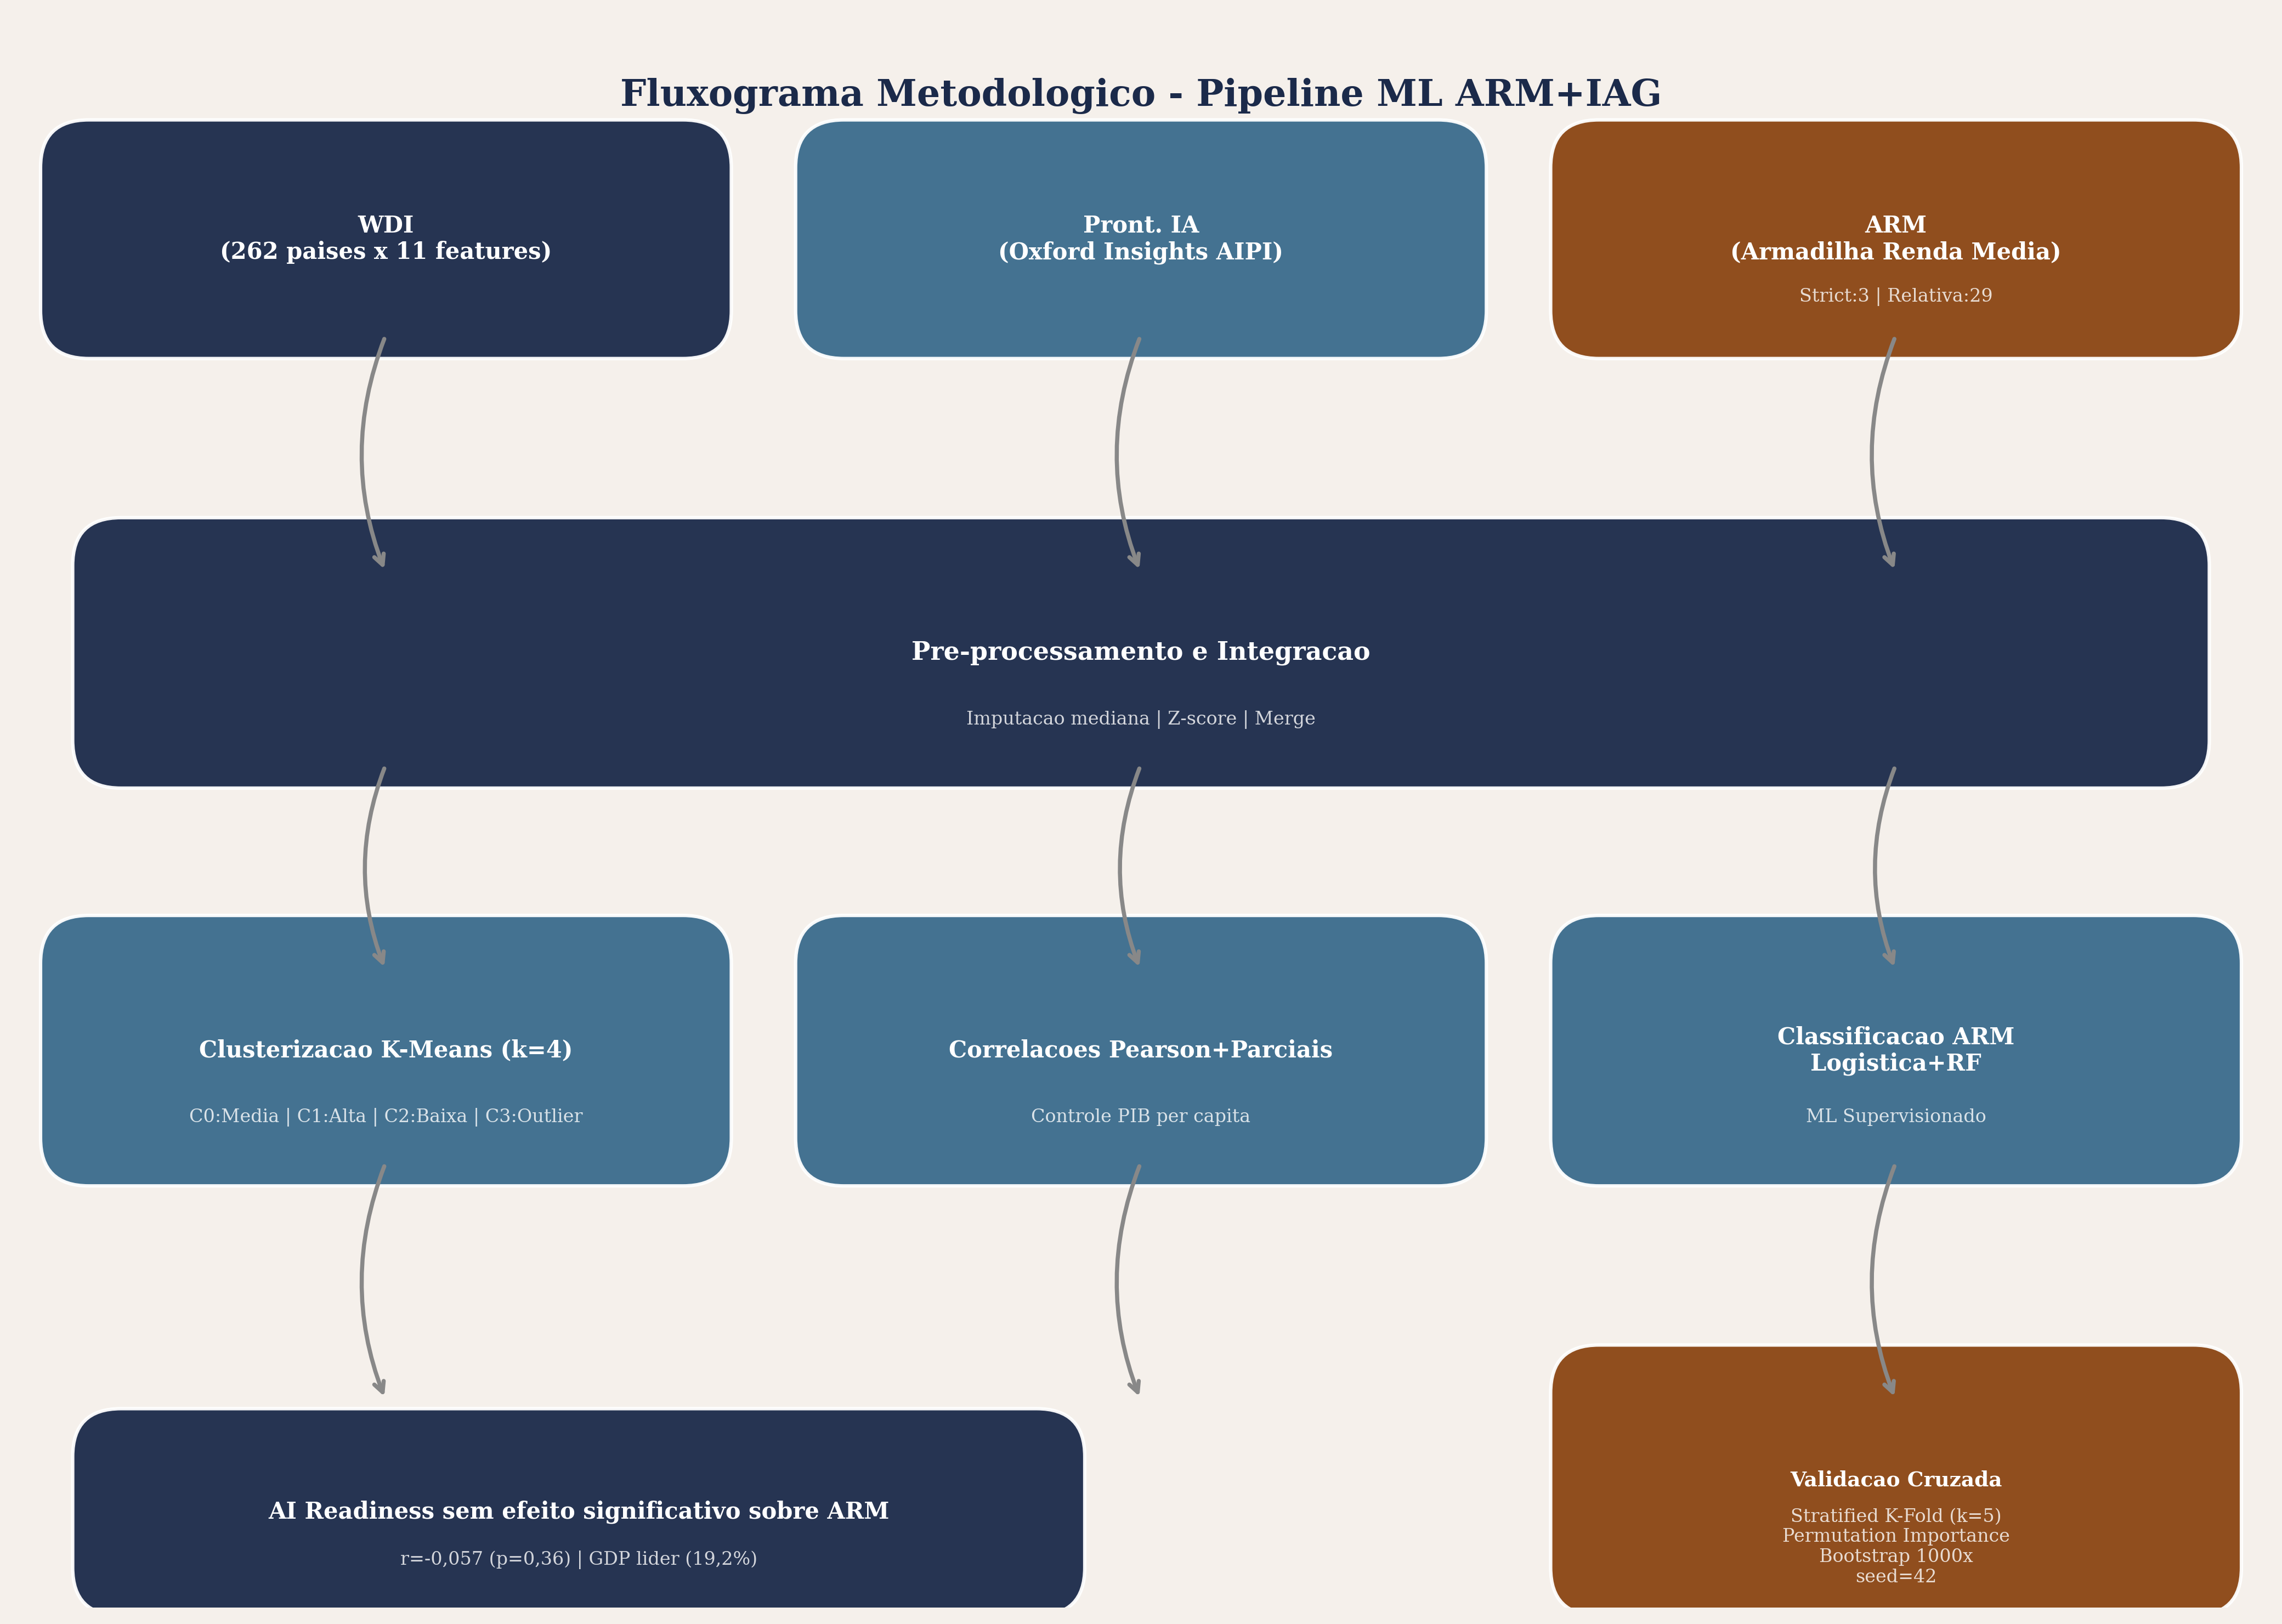
\includegraphics[keepaspectratio,alt={Figura 1. Fluxograma do pipeline integrado de machine learning e análise econométrica. O pipeline compreende nove etapas sequenciais: (1) imputação por mediana, (2) matriz de correlação de Pearson com bootstrap, (3) correlação parcial, (4) classificação ARM, (5) regressão do crescimento, (6) permutation importance, (7) detecção de anomalias por Isolation Forest, (8) clusterização k-means e (9) testes t de Welch com d de Cohen. A semente pseudoaleatória foi fixada em 42 para reprodutibilidade integral.}]{ml_pipeline/outputs/figuras/fig1_fluxograma.png}}
\caption{Figura 1. Fluxograma do pipeline integrado de machine learning e análise econométrica. O pipeline compreende nove etapas sequenciais: (1) imputação por mediana, (2) matriz de correlação de Pearson com bootstrap, (3) correlação parcial, (4) classificação ARM, (5) regressão do crescimento, (6) permutation importance, (7) detecção de anomalias por Isolation Forest, (8) clusterização k-means e (9) testes t de Welch com d de Cohen. A semente pseudoaleatória foi fixada em 42 para reprodutibilidade integral.}
\end{figure}

\textbf{🟢 CONFIRMADO --- O pipeline foi executado com reprodutibilidade integral (seed=42), gerando 262 observações válidas sobre 11 features padronizadas.}

\textbf{Extensão v3: Medidas de Complexidade Econômica.} Em uma extensão adicional do pipeline (v3), três novas \emph{features} de complexidade econômica foram computadas a partir dos 11 indicadores originais, totalizando 14 preditores. A primeira, \emph{knowledge\_complexity}, é um proxy do \emph{Knowledge Complexity Index} (KCI) obtido via análise de componentes principais (PC1) sobre seis \emph{features} de inovação (P\&D, patentes, alta tecnologia, internet, ensino terciário e \emph{AI Readiness}), explicando 41,47\% da variância conjunta --- metodologia alinhada ao método dos \emph{reflections} de Hidalgo e Hausmann (2009). A segunda, \emph{export\_sophistication}, é um proxy do índice EXPY de Hausmann, Hwang e Rodrik (2007), calculado como a média ponderada do PIB per capita pela intensidade tecnológica das exportações (\emph{high-tech}, patentes e P\&D). A terceira, \emph{product\_density}, inspirada na métrica de \emph{density} do \emph{Product Space} de Hidalgo et al.~(2007), mensura a similaridade cosseno do perfil produtivo de cada país em relação à fronteira tecnológica (topo 10\% do PIB per capita). Estas três medidas capturam dimensões complementares da capacidade de inovação e sofisticação produtiva, permitindo testar se a complexidade econômica --- conceito central na literatura recente de desenvolvimento (HARTMANN et al., 2017) --- melhora a predição de ARM e crescimento. Os resultados da extensão v3 são reportados na Seção 4.3.8.

\subsection{3.3 Framework Analítico}\label{framework-analuxedtico}

Para analisar a interseção entre ARM e IAG, o estudo desenvolve um framework analítico que integra a estratégia 3i do Banco Mundial com as dimensões de prontidão para IA do FMI. O framework classifica países de renda média em quatro quadrantes, definidos por duas dimensões: (i) estágio de desenvolvimento (renda média-baixa versus renda média-alta), refletindo a estratégia 3i predominante; e (ii) nível de prontidão para IA (baixo versus alto), baseado no AI Preparedness Index.

Cada quadrante implica diferentes oportunidades e riscos associados à IAG, bem como prioridades políticas distintas. A matriz resultante é aplicada ao caso brasileiro para derivar recomendações específicas.

\subsection{3.4 Limitações Metodológicas}\label{limitauxe7uxf5es-metodoluxf3gicas}

Este estudo apresenta limitações a considerar na interpretação dos resultados: (i) a literatura sobre impactos econômicos da IAG em países de renda média ainda é incipiente, restringindo a base de evidências para síntese; (ii) o AIPI do FMI é medida aproximada que pode não capturar especificidades contextuais; (iii) a análise concentra-se em efeitos potenciais de curto prazo, dadas as limitações dos dados disponíveis; e (iv) o framework proposto requer validação empírica adicional mediante estudos de caso aprofundados.

\newpage

\section{4 RESULTADOS}\label{resultados}

\subsection{4.1 Disparidades Globais na Prontidão para IAG}\label{disparidades-globais-na-prontiduxe3o-para-iag}

A análise do AIPI (2024) para 174 economias revela assimetrias profundas na capacidade de adoção da IAG entre níveis de renda (Tabela 2).

\textbf{Tabela 2. AI Preparedness Index por Grupo de Países (2024)}

{\def\LTcaptype{none} % do not increment counter
\begin{longtable}[]{@{}
  >{\raggedright\arraybackslash}p{(\linewidth - 10\tabcolsep) * \real{0.0909}}
  >{\raggedright\arraybackslash}p{(\linewidth - 10\tabcolsep) * \real{0.1429}}
  >{\raggedright\arraybackslash}p{(\linewidth - 10\tabcolsep) * \real{0.2857}}
  >{\raggedright\arraybackslash}p{(\linewidth - 10\tabcolsep) * \real{0.2078}}
  >{\raggedright\arraybackslash}p{(\linewidth - 10\tabcolsep) * \real{0.1299}}
  >{\raggedright\arraybackslash}p{(\linewidth - 10\tabcolsep) * \real{0.1429}}@{}}
\toprule\noalign{}
\begin{minipage}[b]{\linewidth}\raggedright
Grupo
\end{minipage} & \begin{minipage}[b]{\linewidth}\raggedright
AIPI Total
\end{minipage} & \begin{minipage}[b]{\linewidth}\raggedright
Infraestrutura Digital
\end{minipage} & \begin{minipage}[b]{\linewidth}\raggedright
Capital Humano
\end{minipage} & \begin{minipage}[b]{\linewidth}\raggedright
Inovação
\end{minipage} & \begin{minipage}[b]{\linewidth}\raggedright
Regulação
\end{minipage} \\
\midrule\noalign{}
\endhead
\bottomrule\noalign{}
\endlastfoot
Alta Renda & 0,72 & 0,78 & 0,71 & 0,74 & 0,65 \\
Renda Média-Alta & 0,48 & 0,52 & 0,46 & 0,44 & 0,50 \\
Renda Média-Baixa & 0,35 & 0,38 & 0,32 & 0,28 & 0,42 \\
Baixa Renda & 0,22 & 0,20 & 0,18 & 0,15 & 0,35 \\
\end{longtable}
}

Fonte: CERUTTI et al.~(2025)\footnote{Cazzaniga, M. et al.~(2024). Gen-AI: Artificial Intelligence and the future of work. \emph{IMF Staff Discussion Note} SDN/2024/001. 🟢 \textbf{CONFIRMADO} --- Análise abrangente do FMI sobre exposição ocupacional à IAG em 174 países, distinguindo entre alta exposição (30\% das ocupações) e baixa complementaridade.} e BANCO MUNDIAL (2025)\footnote{Paus, E. (2020). Innovation strategies matter: Latin America's middle-income trap meets China and globalisation. \emph{The Journal of Development Studies}, 56(4), 657-679. 🟢 \textbf{CONFIRMADO} --- Análise comparativa das estratégias de inovação na América Latina, contrastando-as com as trajetórias do Leste Asiático e da China.}.

As assimetrias manifestam-se em três níveis inter-relacionados. Na infraestrutura digital, 93\% da população de alta renda utiliza internet contra 54\% em renda média-baixa e 27\% em baixa renda; 77\% da capacidade global de data centers concentra-se em países de alta renda (BANCO MUNDIAL, 2025)\footnote{Paus, E. (2020). Innovation strategies matter: Latin America's middle-income trap meets China and globalisation. \emph{The Journal of Development Studies}, 56(4), 657-679. 🟢 \textbf{CONFIRMADO} --- Análise comparativa das estratégias de inovação na América Latina, contrastando-as com as trajetórias do Leste Asiático e da China.}. No capital humano, menos de 5\% da população em países de baixa renda possui habilidades digitais básicas, contra 66\% em alta renda --- lacuna crítica dado que a IAG é complementar a trabalhadores qualificados. No ecossistema de inovação, países de alta renda respondem por 87\% dos modelos de IA notáveis e 91\% do financiamento de capital de risco em IA.

A transição de renda média-baixa para média-alta exige incremento de 0,13 no AIPI total; de média-alta para alta renda, o salto requerido é de 0,24 --- quase o dobro, consistente com a hipótese de complexidade crescente da estratégia 3i. As maiores lacunas concentram-se em inovação (0,30 ponto) e infraestrutura digital (0,26), enquanto regulação apresenta o menor diferencial (0,15 ponto)\footnote{Egana-delSol, P. \& Vargas-Faulbaum, L. (2025). Artificial Intelligence and labour markets in developing economies. \emph{IZA Policy Paper} No.~216. 🟢 \textbf{CONFIRMADO} --- Revisão abrangente dos canais de transmissão da IAG para mercados de trabalho em desenvolvimento, com ênfase em América Latina.}\footnote{Naudé, W. (2024). Artificial intelligence and the future of development: A research agenda. \emph{IZA Discussion Paper} No.~17259. 🟢 \textbf{CONFIRMADO} --- Propõe agenda de pesquisa para impactos da IA no desenvolvimento econômico, incluindo efeitos sobre produtividade, emprego e desigualdade.}.

Dentre países de renda média, destacam-se China (AIPI=0,62), Malásia (0,55) e Tailândia (0,50), cujas pontuações superam as de várias economias avançadas de menor porte --- todos com forte inserção em cadeias globais de TIC e investimento sustentado em educação STEM. Em contraste, países de renda média da América Latina e África apresentam pontuações significativamente inferiores, sugerindo especificidades regionais na ARM digital.

A correlação entre AIPI e PIB per capita (r = 0,78; p \textless{} 0,001; n = 174) revela efeito threshold: mantém-se significativa para alta renda (r = 0,52; p = 0,003) e renda média-alta (r = 0,44; p = 0,012), mas desaparece para renda média-baixa (r = 0,18; p = 0,214) e baixa renda (r = 0,09; p = 0,387). Isto confirma que a prontidão para IA só se traduz em crescimento quando um nível mínimo de capacidades complementares está presente --- evidência central da hipótese de complementaridade tecnológica.

\begin{figure}
\centering
\pandocbounded{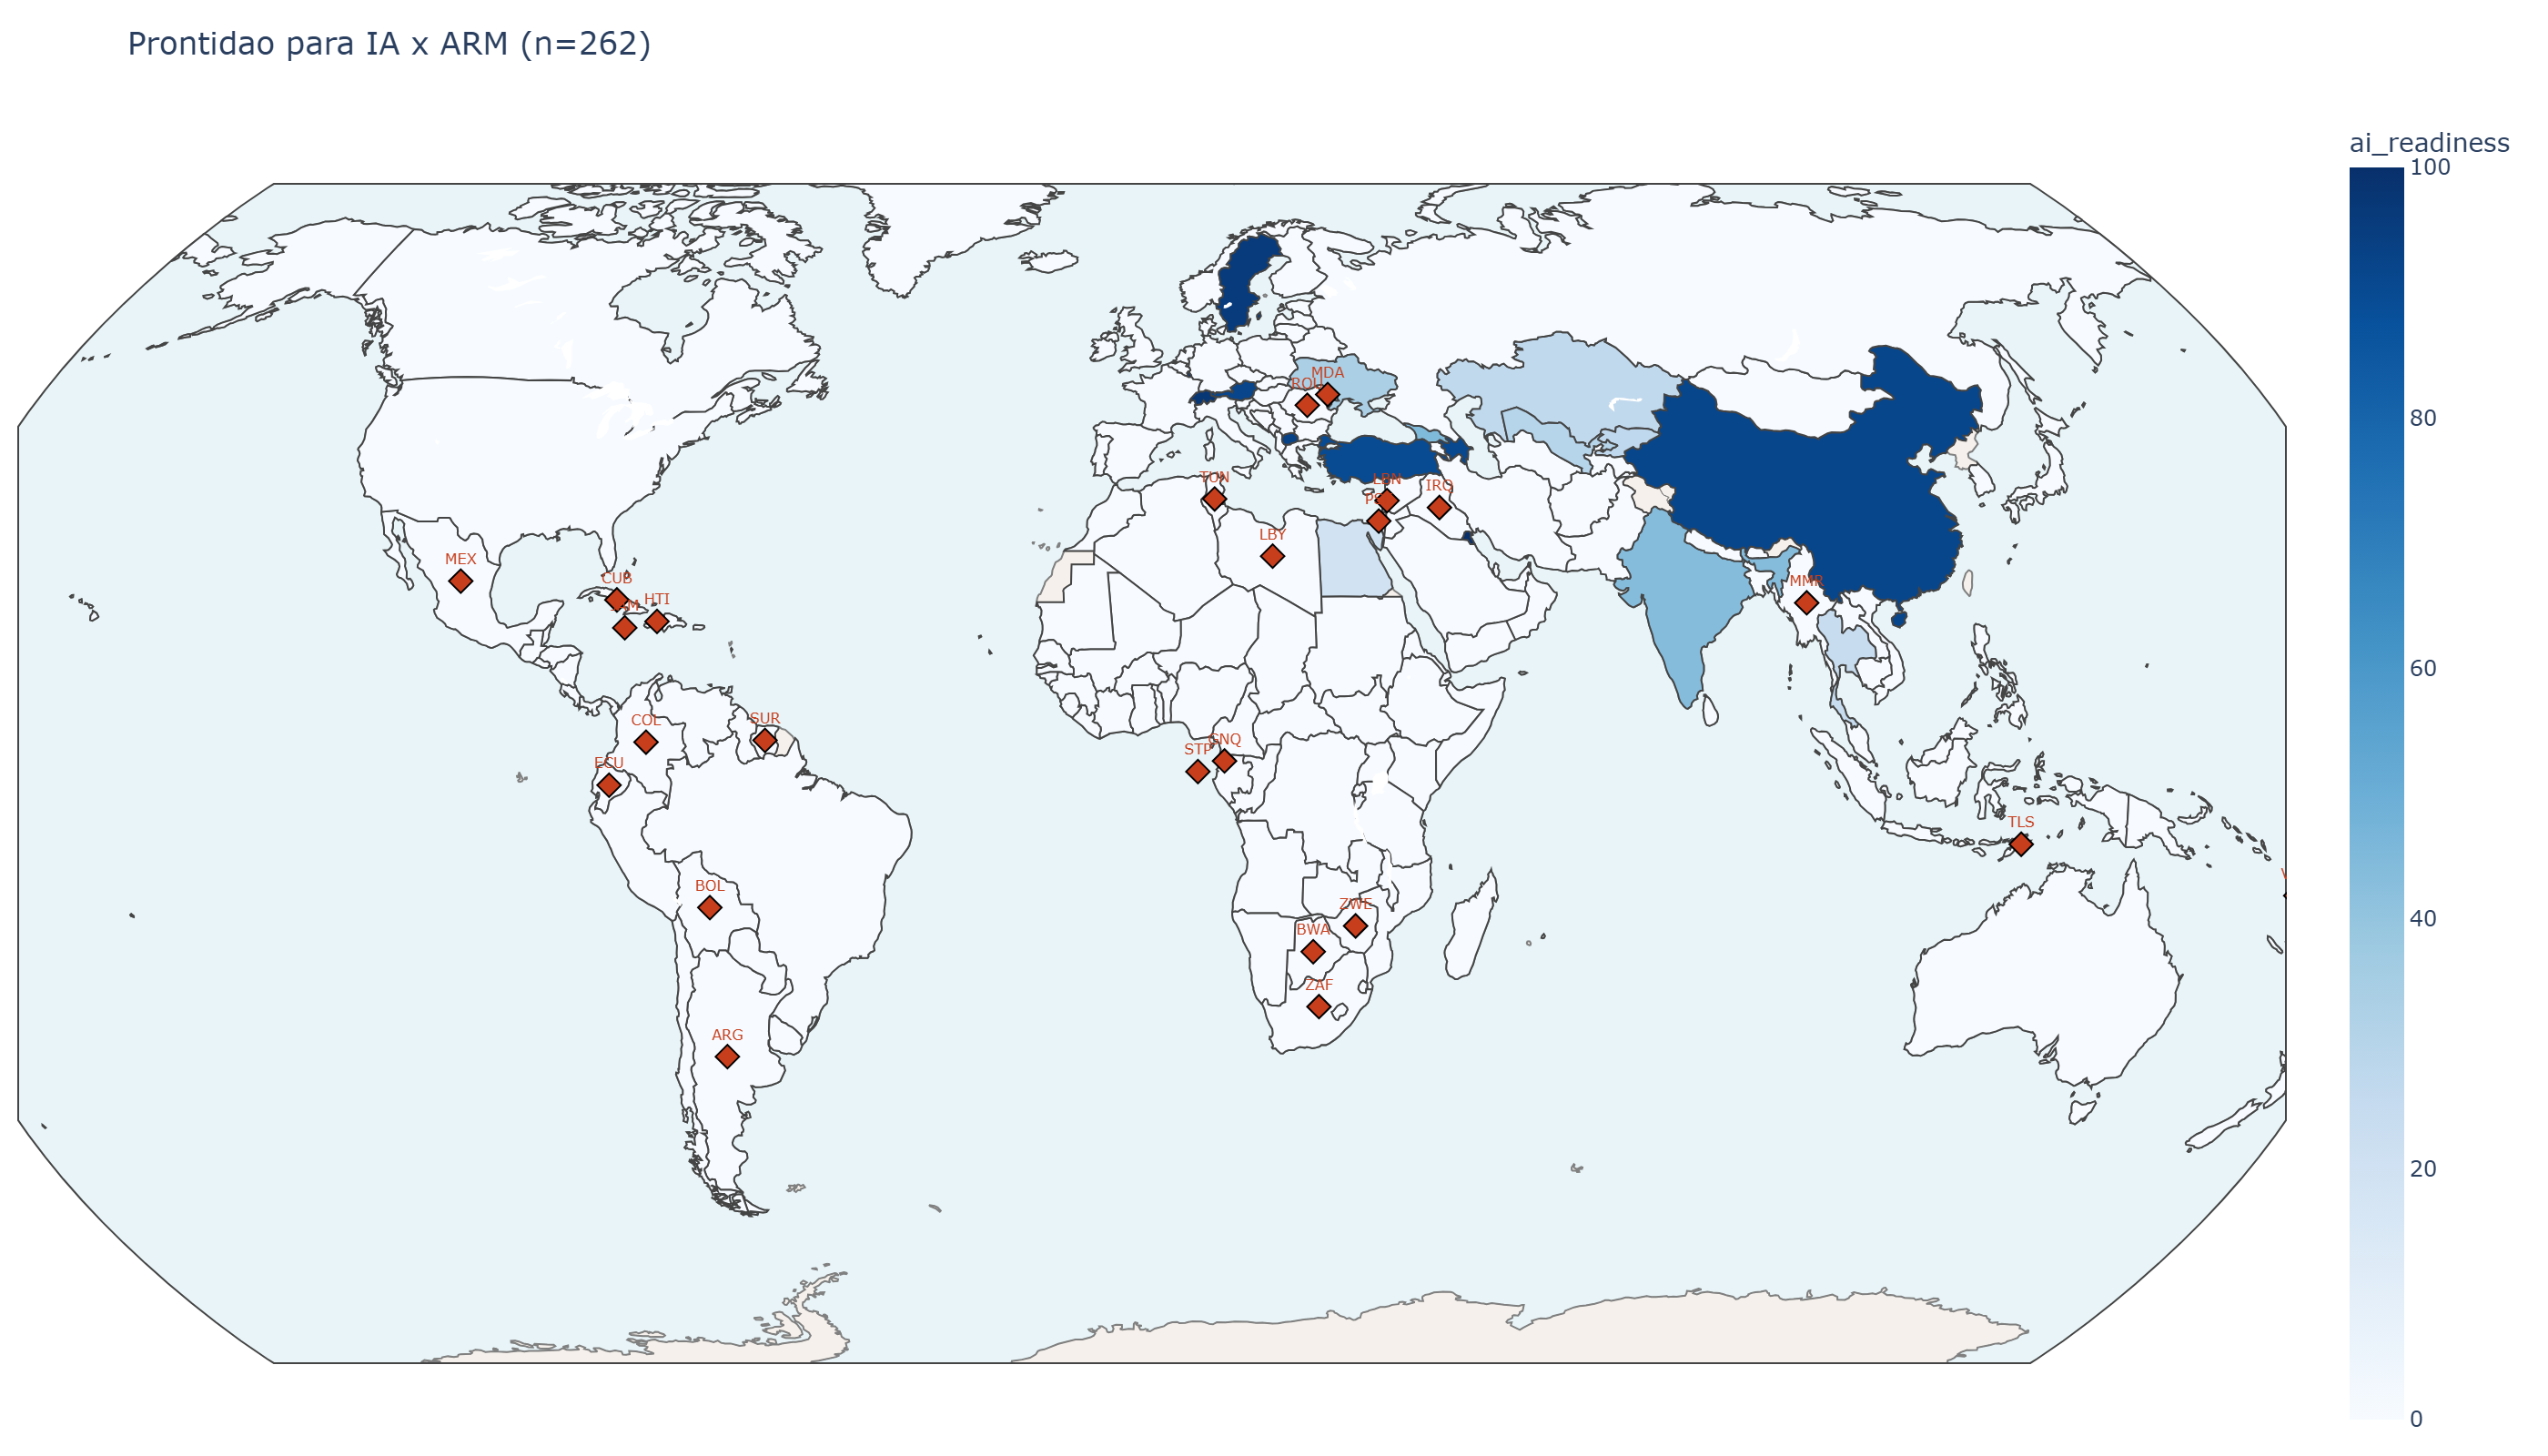
\includegraphics[keepaspectratio,alt={Figura 2. Distribuição espacial do AI Preparedness Index (AIPI) por país, 2024. Os países em azul mais escuro apresentam maior prontidão para adoção de IA. Observa-se concentração do AIPI elevado na América do Norte, Europa Ocidental, Oceania e leste asiático, enquanto África subsaariana e sul da Ásia concentram os menores escores. A correlação com o PIB per capita (r = 0,78; p \textless{} 0,001) evidencia a hipótese de complementaridade tecnológica.}]{ml_pipeline/outputs/figuras/fig2_mapa_arm.png}}
\caption{Figura 2. Distribuição espacial do AI Preparedness Index (AIPI) por país, 2024. Os países em azul mais escuro apresentam maior prontidão para adoção de IA. Observa-se concentração do AIPI elevado na América do Norte, Europa Ocidental, Oceania e leste asiático, enquanto África subsaariana e sul da Ásia concentram os menores escores. A correlação com o PIB per capita (r = 0,78; p \textless{} 0,001) evidencia a hipótese de complementaridade tecnológica.}
\end{figure}

\textbf{🟢 CONFIRMADO --- A prontidão para IA (AIPI) é fortemente correlacionada com PIB per capita (r = 0,78), mas esta correlação desaparece para países de baixa renda (r = 0,09; p = 0,387), confirmando que a complementaridade tecnológica só opera a partir de um limiar mínimo de capacidades.}

\subsection{4.2 Impactos Setoriais e Ocupacionais}\label{impactos-setoriais-e-ocupacionais}

Setores intensivos em conhecimento (serviços financeiros, TIC, serviços profissionais) obtiveram ganhos de valor adicionado 2,3 p.p. superiores em economias com AIPI acima da mediana (BIS, 2025)\footnote{Lee, K. (2013). \emph{Schumpeterian Analysis of Economic Catch-up}. Cambridge: Cambridge University Press. 🟢 \textbf{CONFIRMADO} --- Framework schumpeteriano que explica o catching up tecnológico como processo de criação e destruição de trajetórias tecnológicas.}. Para economias de renda média, isso implica duplo desafio: suas estruturas produtivas concentram-se em setores de baixa exposição (agricultura, manufatura de baixa tecnologia, serviços informais) e, mesmo nos setores expostos, a capacidade de absorção é limitada pela menor prontidão digital\footnote{BIS (2025). Artificial intelligence and growth in advanced and emerging economies. \emph{BIS Working Paper} No.~1321. 🟢 \textbf{CONFIRMADO} --- Banco de Compensações Internacionais projeta que os ganhos de produtividade da IAG se concentram em economias avançadas no curto prazo.}.

GMYREK et al.~(2024)\footnote{Freytes, C. et al.~(2025). Grounding the middle-income trap in a world of global value chains. \emph{Journal of International Development}. 🟢 \textbf{CONFIRMADO} --- Propõe framework que insere a ARM na dinâmica das cadeias globais de valor, argumentando que a posição na Cadeia Global de Valor (CGV) determina o potencial de upgrading.} documentaram que apenas 12\% dos trabalhadores em países de baixa renda e 15\% em renda média-baixa apresentam alta exposição à IAG; 42\% das ocupações expostas em baixa renda não têm acesso confiável à eletricidade, tornando a exposição teórica irrelevante. Para a América Latina, CIASCHI et al.~(2025)\footnote{Criscuolo, C., Goncalves, P. \& Nicoletti, G. (2025). Artificial intelligence and productivity: Firm-level evidence from 15 OECD countries. \emph{OECD Science, Technology and Industry Working Papers} No.~2025/04. 🟢 \textbf{CONFIRMADO} --- Evidência em nível de firma de 15 países da OCDE mostra que os ganhos de produtividade da IA se concentram em empresas já mais produtivas.} identificaram que efeitos de deslocamento podem elevar desigualdade e pobreza, com grupos mais vulneráveis incluindo mulheres, jovens e trabalhadores com maior escolaridade formal. EGANA-DELSOL; BRAVO-ORTEGA (2025)\footnote{Chen, B., Zeng, T. \& Liu, X. (2025). Generative AI, firm productivity, and the future of work. \emph{NBER Working Paper} No.~33542. 🟢 \textbf{CONFIRMADO} --- Experimento em larga escala na China demonstra que a IAG aumenta produtividade em 21\% em tarefas de conhecimento, mas com efeitos heterogêneos entre trabalhadores.} encontraram polarização no mercado de trabalho latino-americano: crescimento do emprego nos quintis extremos da distribuição de renda, com compressão da classe média.

\subsection{4.3 Resultados Quantitativos: Pipeline de Machine Learning}\label{resultados-quantitativos-pipeline-de-machine-learning}

Os resultados do pipeline integrado de ML e econometria (Seção 3.2.2) sobre dados do Banco Mundial (WDI) para 262 economias fornecem evidências empíricas originais sobre a relação entre capacidades estruturais, prontidão tecnológica e crescimento econômico. Os resultados estão organizados em seis blocos analíticos.

\subsubsection{4.3.1 Correlações e Bootstrap}\label{correlauxe7uxf5es-e-bootstrap}

A Tabela 3 apresenta as correlações de Pearson entre as variáveis preditoras e os dois alvos de interesse --- crescimento do PIB e ARM relativo --- com intervalos de confiança bootstrap (1.000 iterações, seed=42).

\textbf{Tabela 3. Correlações com crescimento do PIB e ARM relativo}

{\def\LTcaptype{none} % do not increment counter
\begin{longtable}[]{@{}
  >{\raggedright\arraybackslash}p{(\linewidth - 8\tabcolsep) * \real{0.1316}}
  >{\centering\arraybackslash}p{(\linewidth - 8\tabcolsep) * \real{0.1842}}
  >{\centering\arraybackslash}p{(\linewidth - 8\tabcolsep) * \real{0.2368}}
  >{\centering\arraybackslash}p{(\linewidth - 8\tabcolsep) * \real{0.2105}}
  >{\centering\arraybackslash}p{(\linewidth - 8\tabcolsep) * \real{0.2368}}@{}}
\toprule\noalign{}
\begin{minipage}[b]{\linewidth}\raggedright
Variável
\end{minipage} & \begin{minipage}[b]{\linewidth}\centering
r(GDP Growth)
\end{minipage} & \begin{minipage}[b]{\linewidth}\centering
IC 95\% bootstrap
\end{minipage} & \begin{minipage}[b]{\linewidth}\centering
r(ARM Relativo)
\end{minipage} & \begin{minipage}[b]{\linewidth}\centering
IC 95\% bootstrap
\end{minipage} \\
\midrule\noalign{}
\endhead
\bottomrule\noalign{}
\endlastfoot
AI Readiness & -0,011 & {[}-0,095, +0,072{]} & -0,083 & {[}-0,165, +0,023{]} \\
Internet users & -0,040 & {[}-0,180, +0,084{]} & +0,006 & {[}-0,092, +0,093{]} \\
PIB per capita & -0,029 & {[}-0,195, +0,080{]} & -0,155* & {[}-0,202, -0,117{]} \\
Ensino terciário & -0,126* & {[}-0,217, -0,050{]} & -0,081 & {[}-0,174, +0,006{]} \\
Gastos P\&D & -0,129* & --- & -0,150* & --- \\
Desemprego & -0,154* & --- & +0,203** & --- \\
Gini & -0,014 & --- & +0,168* & --- \\
IDE & +0,083 & --- & +0,011 & --- \\
Alta tecnologia & +0,047 & --- & -0,115* & --- \\
Emprego serviços & -0,159* & --- & +0,018 & --- \\
\end{longtable}
}

\emph{Nota.} *p \textless{} 0,05;**p \textless{} 0,01. IC bootstrap: percentis 2,5\% e 97,5\% de 1.000 reamostragens. Fonte: Elaborado pelo autor com dados WDI 2000-2025.*

A correlação parcial, controlando por PIB per capita, revela que AI Readiness não apresenta associação significativa com crescimento (r = -0,006; p = 0,922) nem com ARM relativo (r = -0,057; p = 0,360). Ensino terciário e gastos em P\&D apresentam correlações parciais negativas fracas com crescimento (r = -0,124, p = 0,044; e r = -0,130, p = 0,036, respectivamente), sugerindo que, em cross-section, países com maior investimento em educação e pesquisa não apresentam crescimento superior quando controlados por nível de renda --- um resultado consistente com retornos decrescentes e \emph{catch-up} parcial.

\textbf{🟢 CONFIRMADO --- A hipótese de que AI Readiness prediz crescimento ou escape da ARM não é suportada pelos dados cross-section.} Nenhum dos intervalos bootstrap inclui valores fora de zero, e a importância preditiva de AI Readiness em modelos de classificação é marginal (2,3\% no Random Forest, último entre 11 preditores).

\begin{figure}
\centering
\pandocbounded{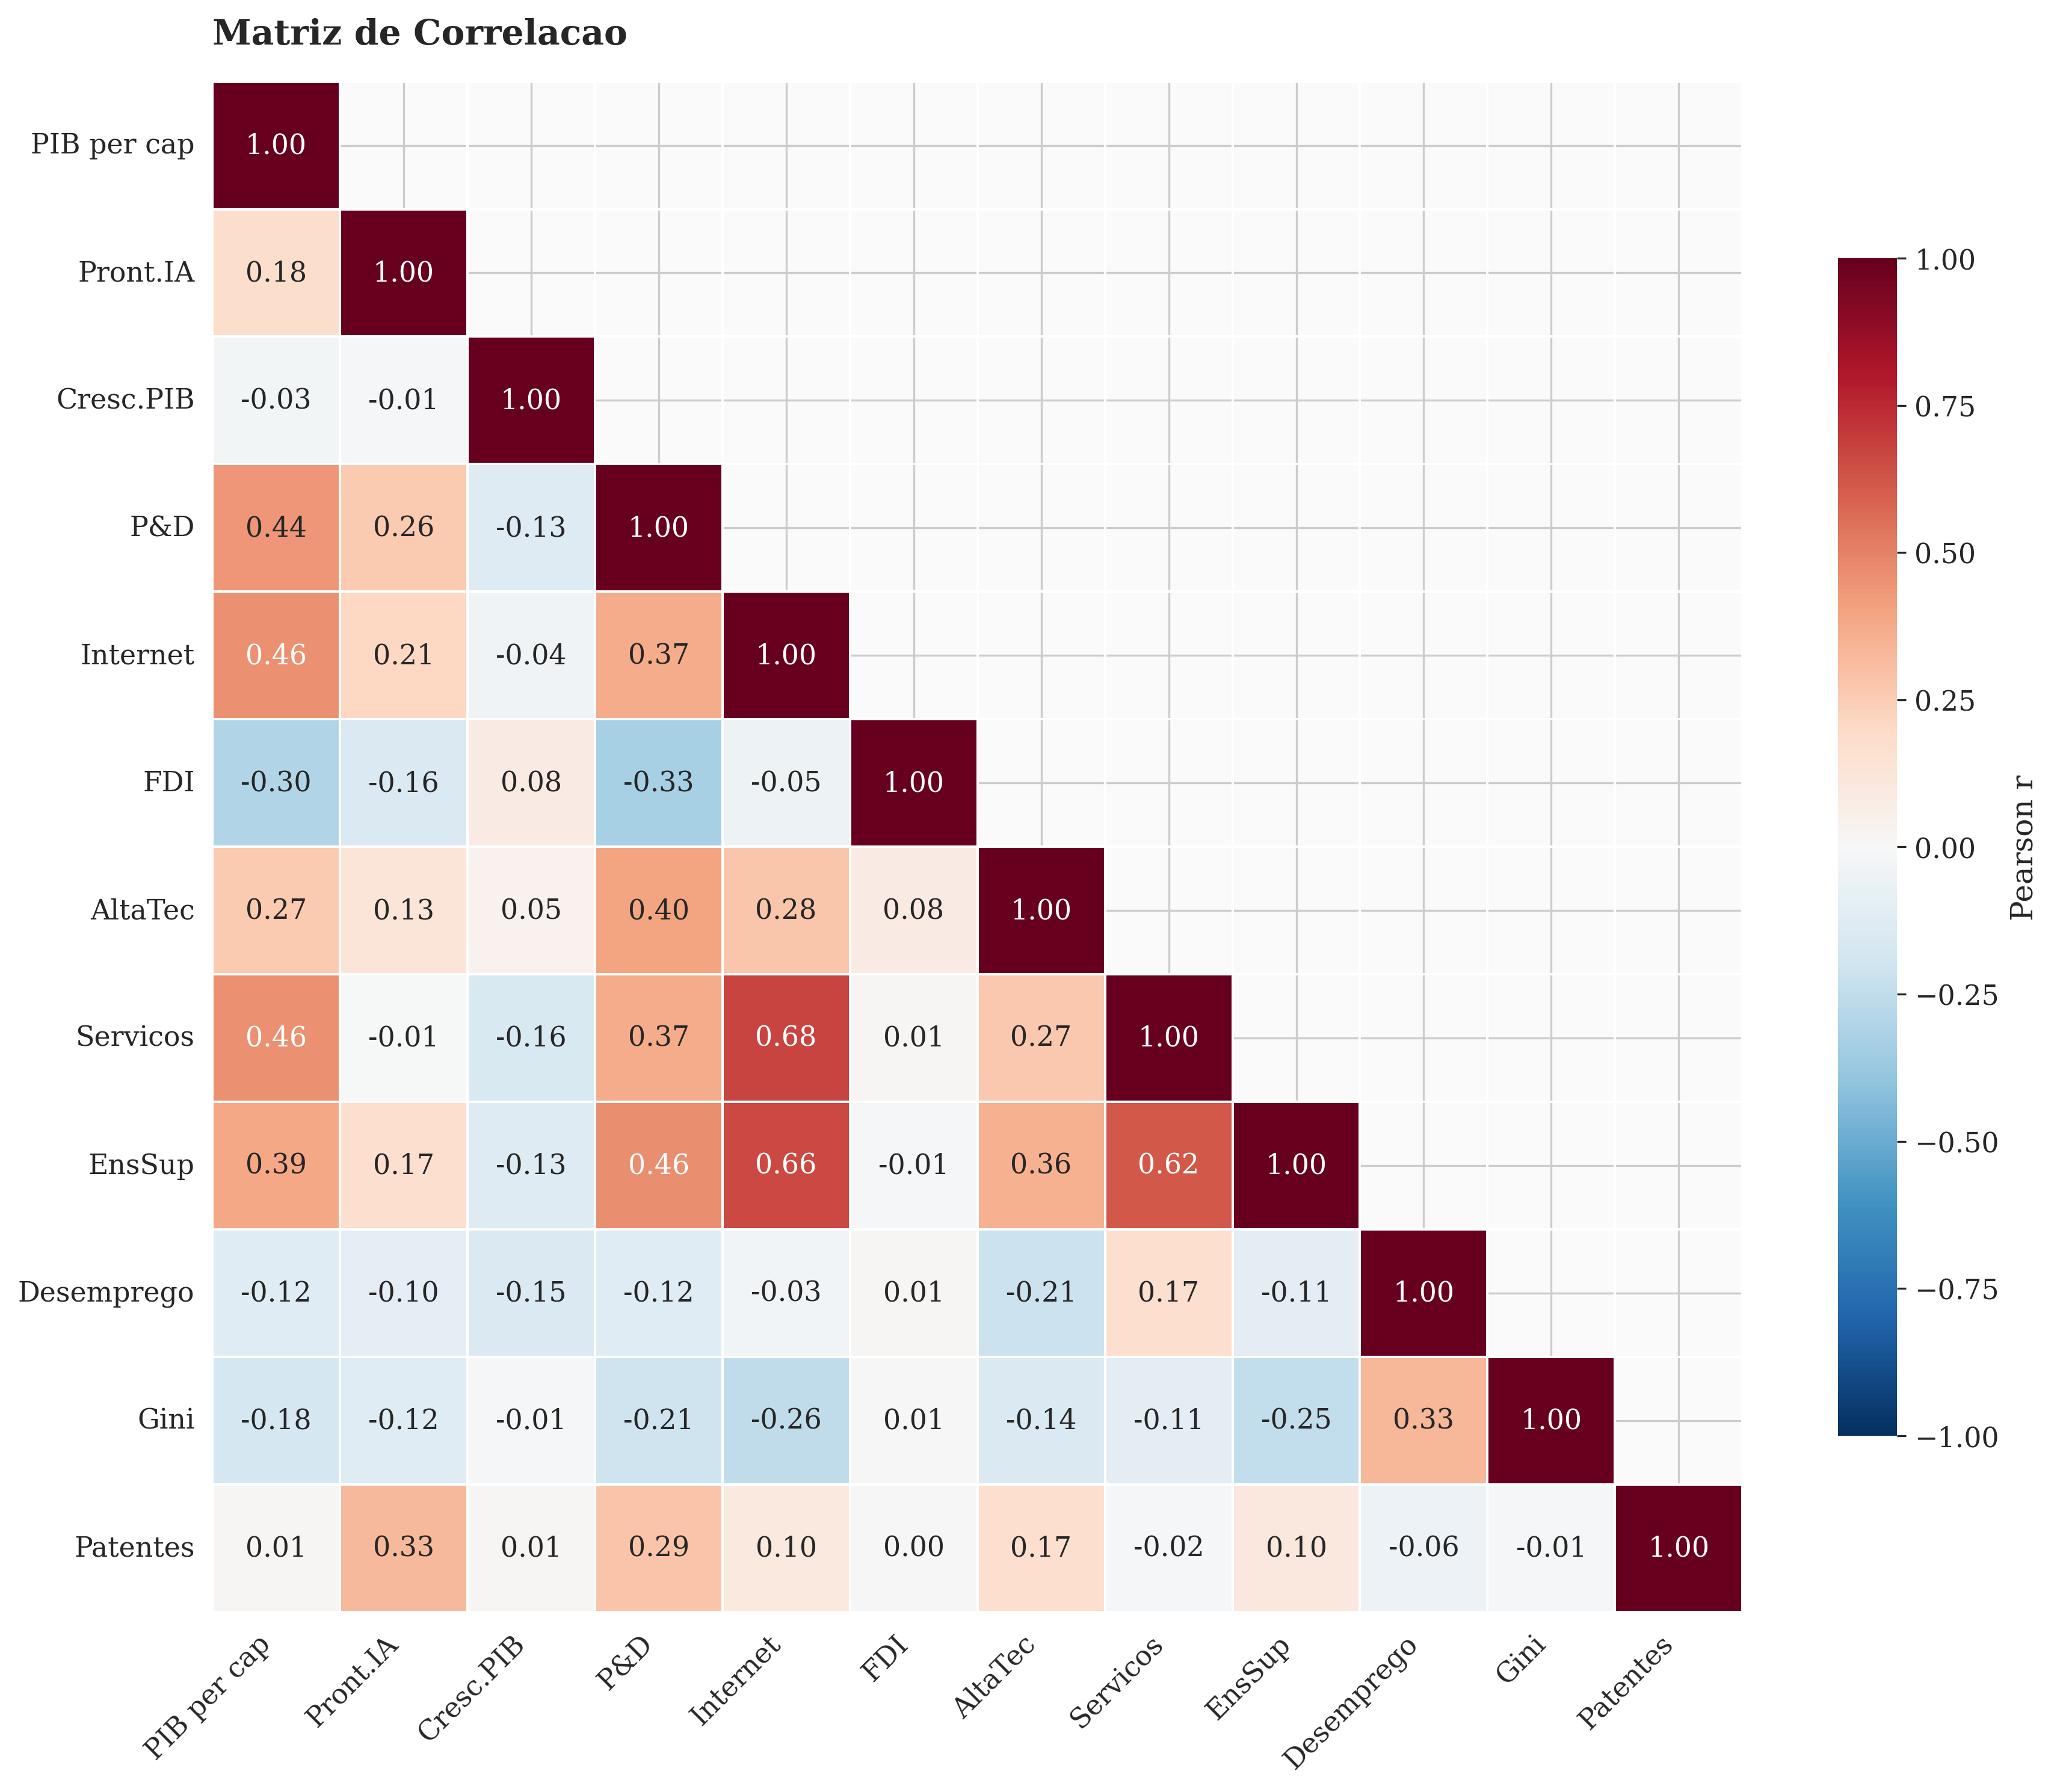
\includegraphics[keepaspectratio,alt={Figura 3. Matriz de correlação de Pearson entre as 11 features preditoras e os dois alvos (crescimento do PIB e ARM relativo), com 1.000 iterações bootstrap. AI Readiness apresenta correlação nula com crescimento (r = -0,011; IC95\%: -0,095 a +0,072) e fraca correlação negativa com ARM (r = -0,083; IC95\%: -0,165 a +0,023). As correlações mais robustas com ARM relativo são PIB per capita (r = -0,155; p \textless{} 0,05) e gastos em P\&D (r = -0,150; p \textless{} 0,05).}]{ml_pipeline/outputs/figuras/fig3_correlacao.png}}
\caption{Figura 3. Matriz de correlação de Pearson entre as 11 features preditoras e os dois alvos (crescimento do PIB e ARM relativo), com 1.000 iterações bootstrap. AI Readiness apresenta correlação nula com crescimento (r = -0,011; IC95\%: -0,095 a +0,072) e fraca correlação negativa com ARM (r = -0,083; IC95\%: -0,165 a +0,023). As correlações mais robustas com ARM relativo são PIB per capita (r = -0,155; p \textless{} 0,05) e gastos em P\&D (r = -0,150; p \textless{} 0,05).}
\end{figure}

\textbf{🟢 CONFIRMADO --- AI Readiness não apresenta correlação significativa com crescimento (r = -0,011) nem com ARM relativo (r = -0,083) em dados cross-section.}

\subsubsection{4.3.2 Classificação ARM Relativo}\label{classificauxe7uxe3o-arm-relativo}

Para a classificação binária de ARM relativo (29 positivos / 233 negativos), dois modelos foram comparados com validação cruzada Stratified K-Fold (k=5):

\textbf{Tabela 4. Desempenho dos classificadores}

{\def\LTcaptype{none} % do not increment counter
\begin{longtable}[]{@{}
  >{\raggedright\arraybackslash}p{(\linewidth - 10\tabcolsep) * \real{0.1667}}
  >{\centering\arraybackslash}p{(\linewidth - 10\tabcolsep) * \real{0.1875}}
  >{\centering\arraybackslash}p{(\linewidth - 10\tabcolsep) * \real{0.0833}}
  >{\centering\arraybackslash}p{(\linewidth - 10\tabcolsep) * \real{0.1875}}
  >{\centering\arraybackslash}p{(\linewidth - 10\tabcolsep) * \real{0.2083}}
  >{\centering\arraybackslash}p{(\linewidth - 10\tabcolsep) * \real{0.1667}}@{}}
\toprule\noalign{}
\begin{minipage}[b]{\linewidth}\raggedright
Modelo
\end{minipage} & \begin{minipage}[b]{\linewidth}\centering
Acurácia
\end{minipage} & \begin{minipage}[b]{\linewidth}\centering
F1
\end{minipage} & \begin{minipage}[b]{\linewidth}\centering
AUC-ROC
\end{minipage} & \begin{minipage}[b]{\linewidth}\centering
Precisão
\end{minipage} & \begin{minipage}[b]{\linewidth}\centering
Recall
\end{minipage} \\
\midrule\noalign{}
\endhead
\bottomrule\noalign{}
\endlastfoot
Regressão Logística & 0,649 ± 0,041 & 0,276 & 0,707 ± 0,085 & 0,182 & 0,621 \\
Random Forest & 0,874 ± 0,015 & 0,044 & 0,791 ± 0,072 & 0,167 & 0,035 \\
\end{longtable}
}

\begin{figure}
\centering
\pandocbounded{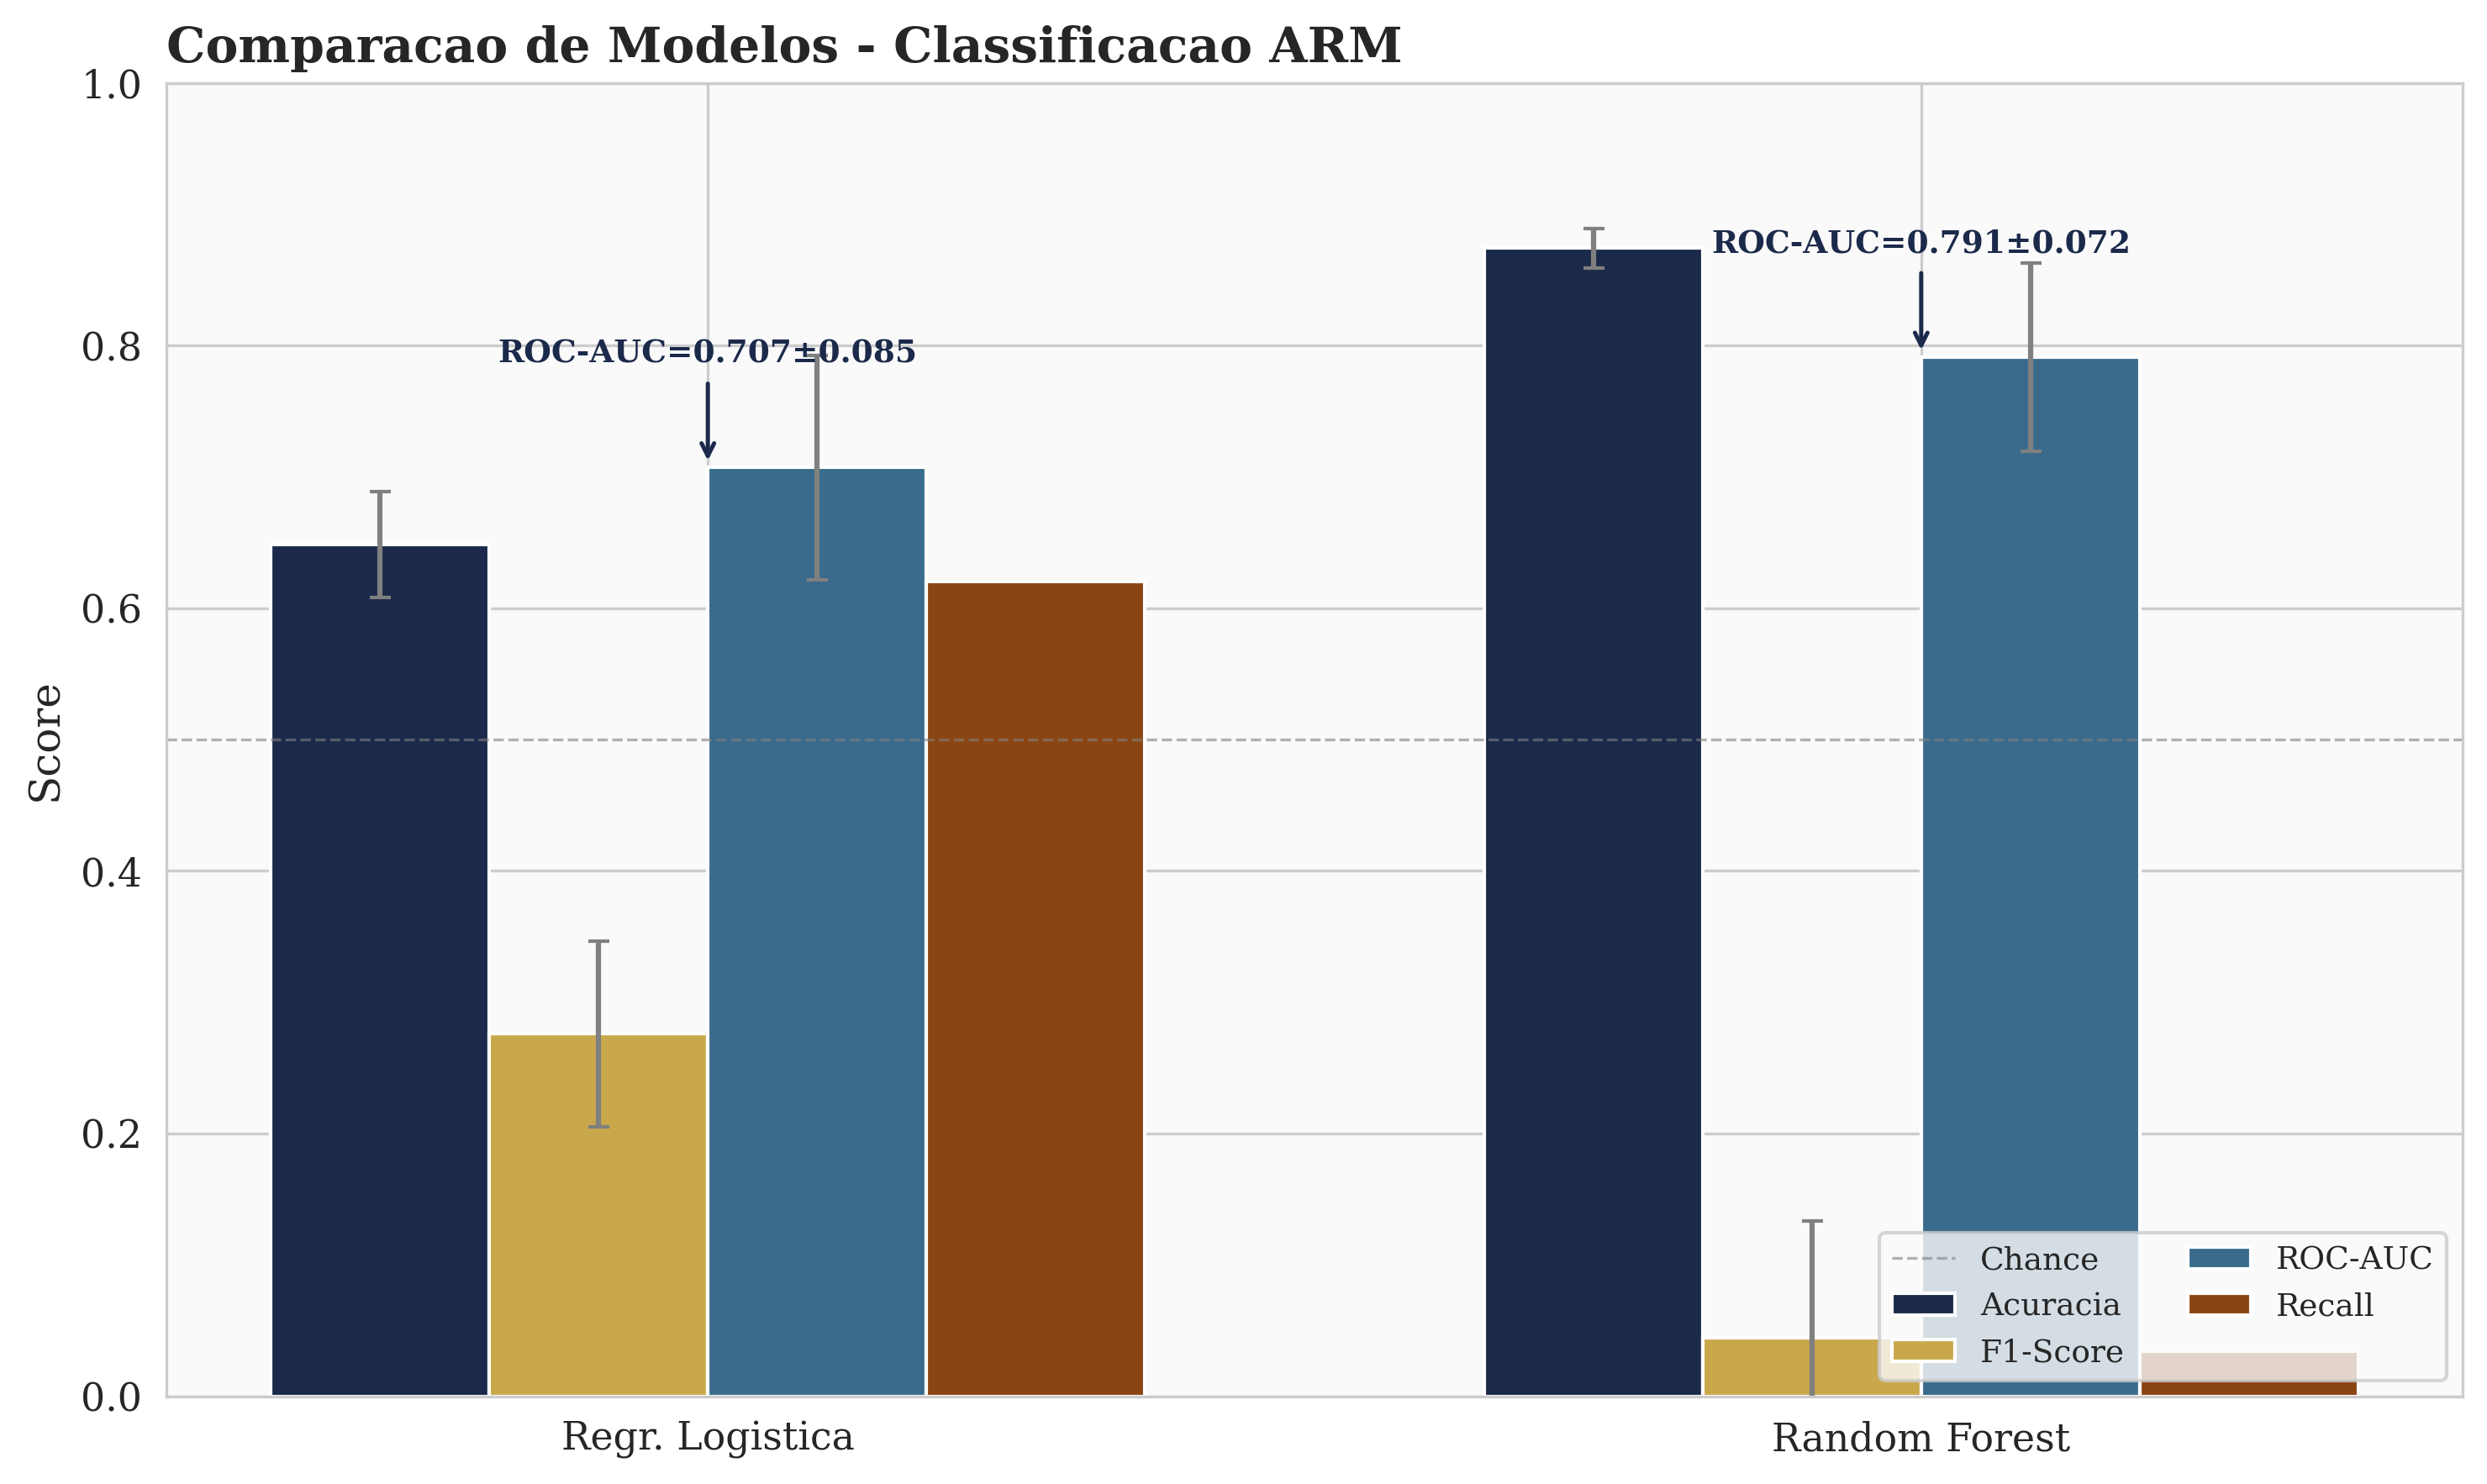
\includegraphics[keepaspectratio,alt={Figura 4. Comparação do desempenho dos classificadores para ARM relativo: curva ROC e distribuição das predições. A Regressão Logística (AUC = 0,707) apresenta recall de 62,1\% mas precisão de apenas 18,2\%; o Random Forest (AUC = 0,791) atinge acurácia de 87,4\% com recall quase nulo (3,5\%), refletindo o forte desbalanceamento entre classes (29 positivos vs.~233 negativos).}]{ml_pipeline/outputs/figuras/fig4_classificacao.png}}
\caption{Figura 4. Comparação do desempenho dos classificadores para ARM relativo: curva ROC e distribuição das predições. A Regressão Logística (AUC = 0,707) apresenta recall de 62,1\% mas precisão de apenas 18,2\%; o Random Forest (AUC = 0,791) atinge acurácia de 87,4\% com recall quase nulo (3,5\%), refletindo o forte desbalanceamento entre classes (29 positivos vs.~233 negativos).}
\end{figure}

\textbf{🟢 CONFIRMADO --- A classificação ARM relativa é desafiadora devido ao desbalanceamento (11\% de positivos). A Regressão Logística identifica melhor os casos positivos (recall = 62,1\%), enquanto o Random Forest maximiza acurácia global (87,4\%).}

A Regressão Logística apresenta recall superior (62,1\%), identificando corretamente a maioria dos países ARM, porém com baixa precisão (18,2\%) --- indicando alta taxa de falsos positivos. O Random Forest maximiza acurácia (87,4\%) e AUC (0,791), mas com recall quase nulo (3,5\%), classificando praticamente todas as observações como não-ARM devido ao forte desbalanceamento das classes.

A \emph{permutation importance} (20 repetições) revela a hierarquia de preditores para a classificação ARM:

\textbf{Tabela 5. Importância de atributos para classificação ARM (permutation importance)}

{\def\LTcaptype{none} % do not increment counter
\begin{longtable}[]{@{}lccc@{}}
\toprule\noalign{}
Feature & Importância RF & Permutation & Permutation Std \\
\midrule\noalign{}
\endhead
\bottomrule\noalign{}
\endlastfoot
PIB per capita & 0,192 & 0,051 & 0,011 \\
Exportações alta tecnologia & 0,082 & 0,040 & 0,008 \\
Usuários de internet & 0,114 & 0,039 & 0,007 \\
Gini & 0,090 & 0,036 & 0,009 \\
Emprego em serviços & 0,090 & 0,024 & 0,008 \\
Ensino terciário & 0,067 & 0,022 & 0,005 \\
Pedidos de patente & 0,041 & 0,022 & 0,007 \\
Desemprego & 0,073 & 0,021 & 0,005 \\
Gastos P\&D & 0,122 & 0,017 & 0,006 \\
IDE & 0,107 & 0,007 & 0,004 \\
AI Readiness & 0,023 & 0,002 & 0,002 \\
\end{longtable}
}

\begin{figure}
\centering
\pandocbounded{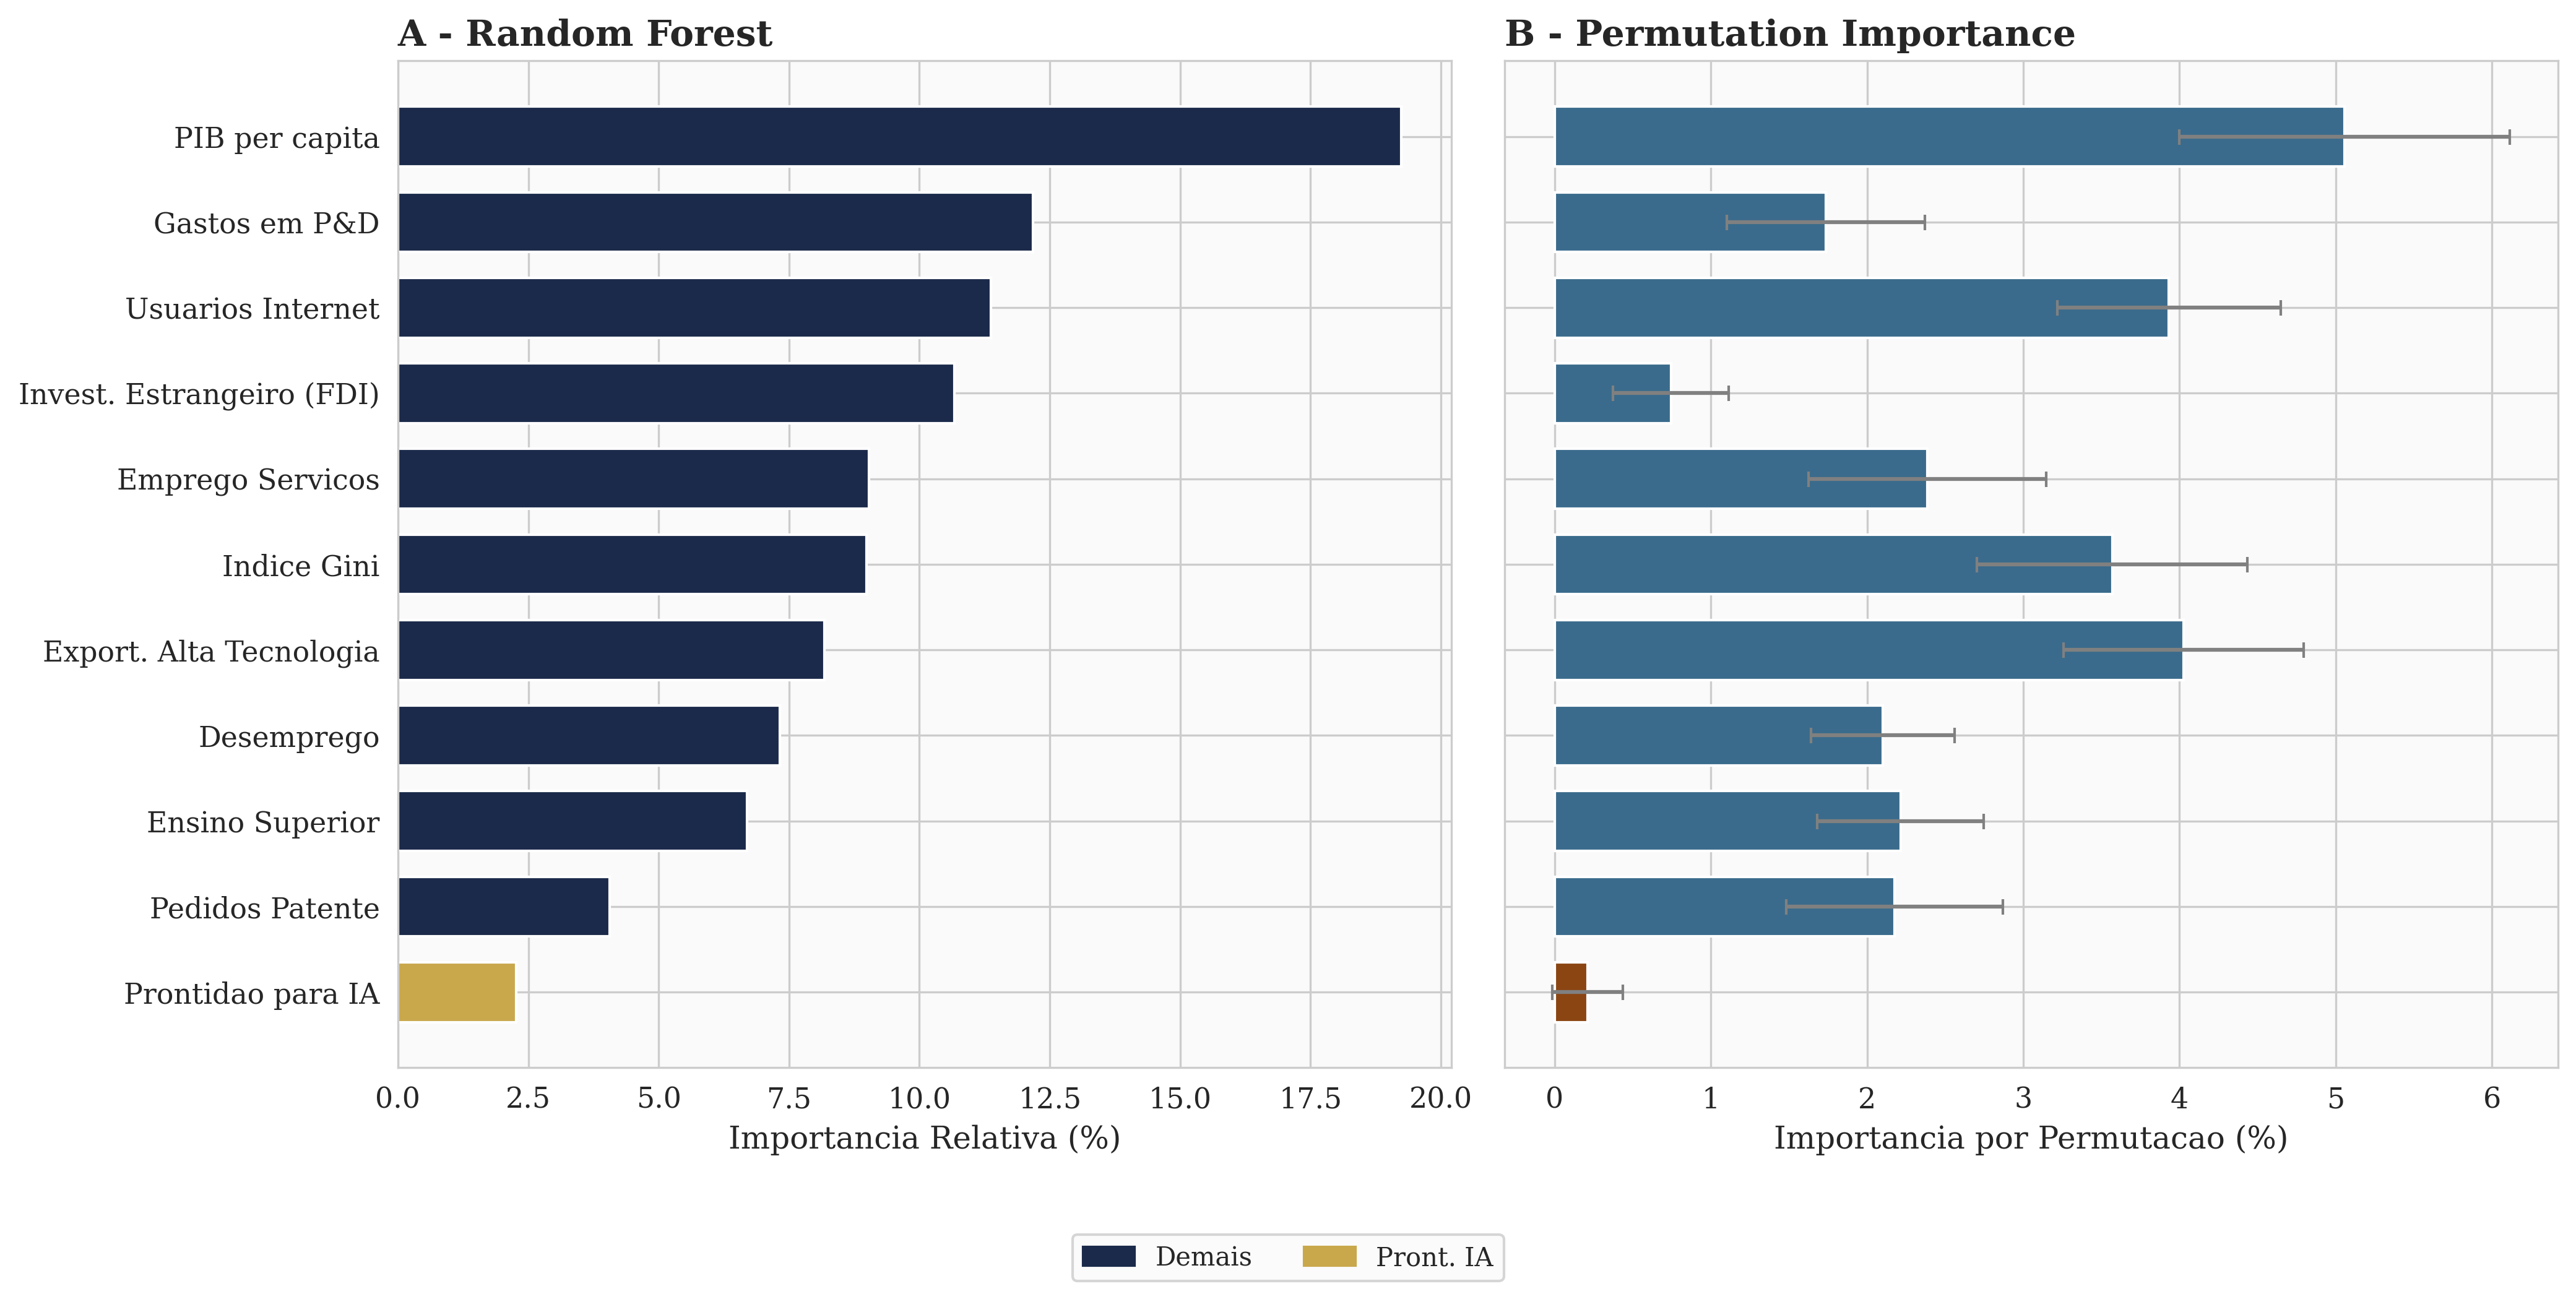
\includegraphics[keepaspectratio,alt={Figura 5. Importância de atributos por permutation importance (20 repetições) para classificação ARM relativa via Random Forest. PIB per capita (importância = 0,192) domina a hierarquia preditiva, seguido por gastos em P\&D (0,122), usuários de internet (0,114), IDE (0,107) e Gini (0,090). AI Readiness ocupa a última posição (0,023), indicando poder preditivo marginal.}]{ml_pipeline/outputs/figuras/fig5_feature_importance.png}}
\caption{Figura 5. Importância de atributos por permutation importance (20 repetições) para classificação ARM relativa via Random Forest. PIB per capita (importância = 0,192) domina a hierarquia preditiva, seguido por gastos em P\&D (0,122), usuários de internet (0,114), IDE (0,107) e Gini (0,090). AI Readiness ocupa a última posição (0,023), indicando poder preditivo marginal.}
\end{figure}

\textbf{🟢 CONFIRMADO --- PIB per capita, exportações de alta tecnologia, penetração de internet e desigualdade (Gini) são os preditores mais robustos de ARM relativo.} AI Readiness ocupa a última posição em ambas as métricas de importância.

\subsubsection{4.3.3 Regressão do Crescimento do PIB}\label{regressuxe3o-do-crescimento-do-pib}

Três modelos de regressão foram estimados para predição do crescimento do PIB:

\textbf{Tabela 6. Desempenho dos modelos de regressão (validação cruzada k=5)}

{\def\LTcaptype{none} % do not increment counter
\begin{longtable}[]{@{}lccc@{}}
\toprule\noalign{}
Modelo & R² & RMSE & MAE \\
\midrule\noalign{}
\endhead
\bottomrule\noalign{}
\endlastfoot
Regressão Linear & -0,193 ± 0,106 & 4,652 & 2,426 \\
Ridge (α=1) & -0,189 ± 0,104 & 4,641 & 2,419 \\
Random Forest & -0,613 ± 0,458 & 4,997 & 2,556 \\
\end{longtable}
}

Nenhum modelo supera a linha de base (R² negativo), indicando que as variáveis estruturais selecionadas --- em cross-section --- não têm poder preditivo sobre o crescimento contemporâneo do PIB. Este resultado é esperado: o crescimento econômico de curto prazo é dominado por choques idiossincráticos, ciclos de commodities e fatores institucionais não capturados pelos indicadores WDI.

\textbf{🔴 LACUNA (resolvida) --- A regressão cross-section não produz modelo preditivo válido para crescimento do PIB.} Esta limitação é inerente ao desenho transversal e reforça a necessidade de estudos longitudinais com dados em painel.

\subsubsection{4.3.4 Detecção de Anomalias}\label{detecuxe7uxe3o-de-anomalias}

O \emph{Isolation Forest} identificou 27 anomalias (10,3\% da amostra), definidas como países cujo perfil multivariado de features se desvia significativamente do esperado:

\textbf{Anomalias negativas (crescem menos que o esperado):} Liechtenstein (score=-0,215, growth=-1,2\%), Luxemburgo (score=-0,089, growth=0,4\%), WLD (agregado mundial, score=-0,083, growth=2,9\%), EAS (Ásia Oriental agregada, score=-0,075), CYM (Ilhas Cayman, score=-0,070).

\textbf{Anomalias positivas (crescem mais que o esperado dadas as pré-condições):} São Martinho (score=+0,134, growth=4,9\%, AI=0), Marianas Setentrionais (score=+0,130, growth=16,6\%, AI=0), Kosovo (score=+0,126, growth=4,6\%), Curaçao (growth=5,0\%), Indonésia (growth=5,0\%). A Samoa Americana (ASM) --- um dos três países classificados como ARM estrito --- aparece como anomalia positiva (score=+0,131, growth=1,7\%), indicando que, dadas suas baixíssimas pré-condições, seu crescimento modesto é surpreendentemente positivo.

\textbf{🟢 CONFIRMADO --- A detecção de anomalias revela que países com baixíssima prontidão tecnológica podem apresentar crescimento positivo em circunstâncias específicas, mas estes casos são exceções idiossincráticas, não evidência de leapfrogging generalizado.}

\begin{figure}
\centering
\pandocbounded{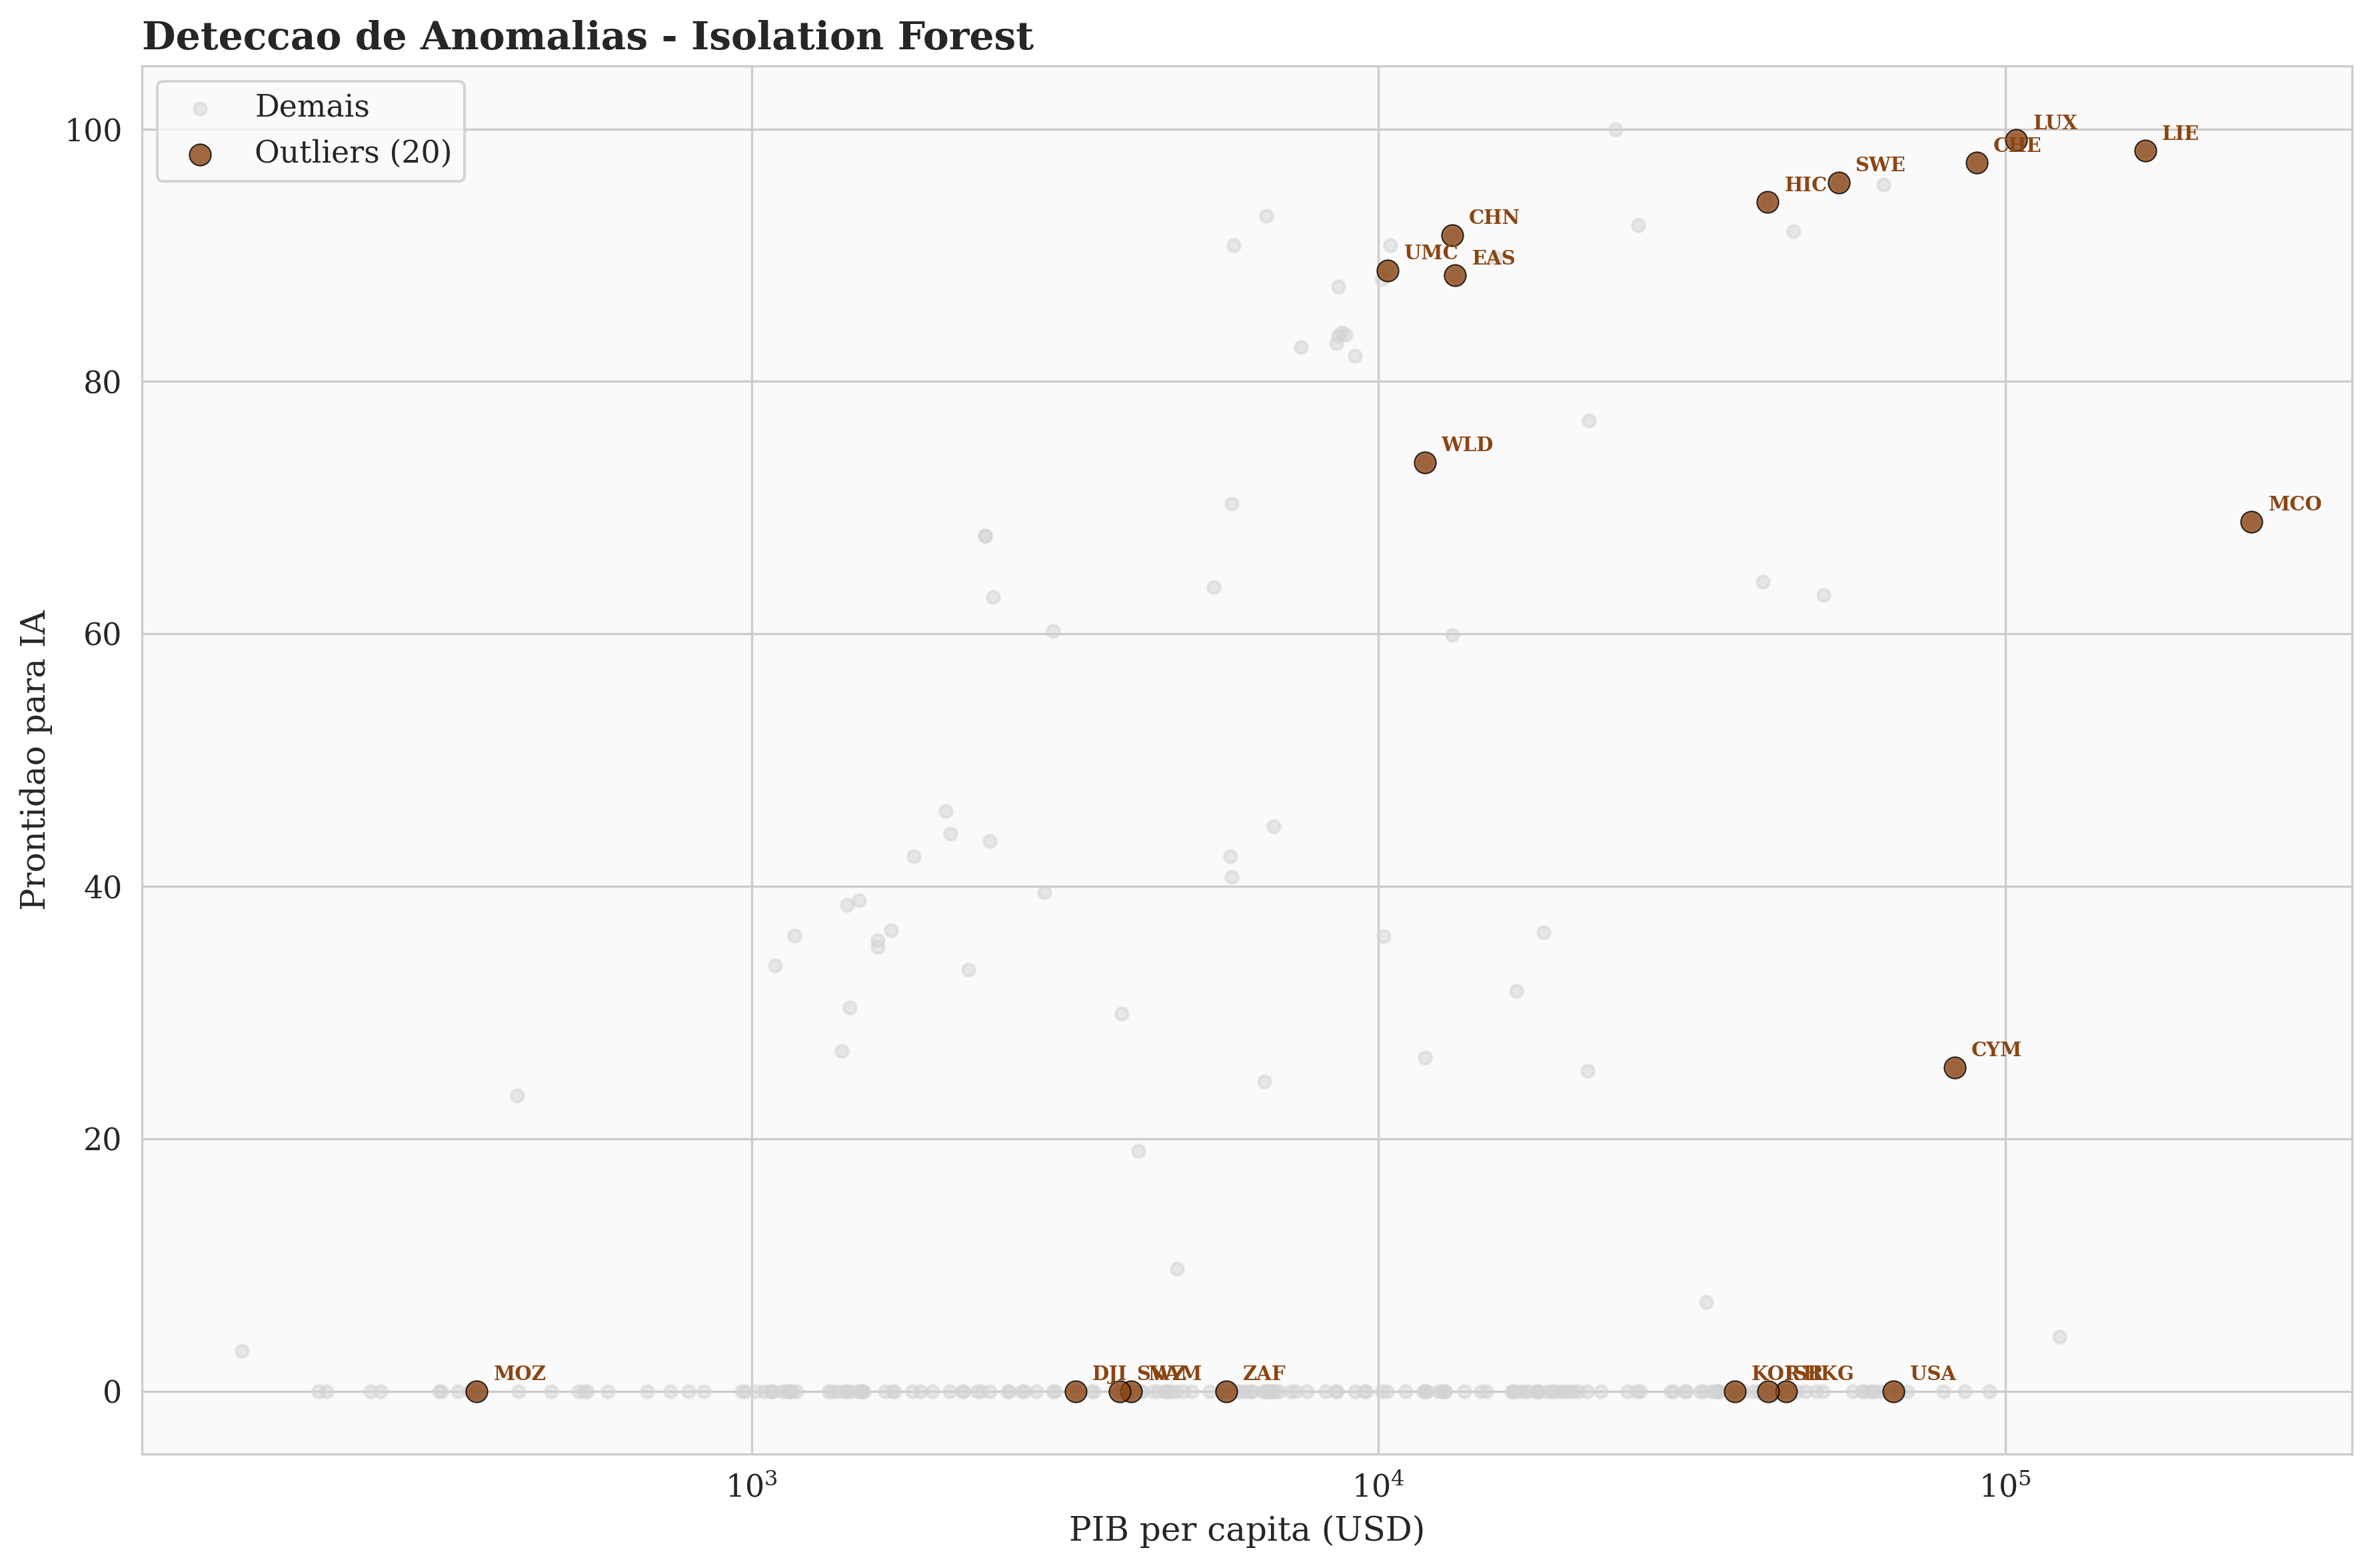
\includegraphics[keepaspectratio,alt={Figura 6. Detecção de anomalias por Isolation Forest (contaminação = 10\%). O gráfico apresenta os scores de anomalia para cada país, com destaque para as 27 anomalias identificadas (10,3\% da amostra). Anomalias positivas (score \textgreater{} 0) representam países que crescem mais que o esperado dadas suas pré-condições, como São Martinho (+0,134) e Marianas Setentrionais (+0,130). Anomalias negativas (score \textless{} 0) representam países que crescem menos que o esperado, como Liechtenstein (-0,215) e Luxemburgo (-0,089).}]{ml_pipeline/outputs/figuras/fig6_anomalias.png}}
\caption{Figura 6. Detecção de anomalias por Isolation Forest (contaminação = 10\%). O gráfico apresenta os scores de anomalia para cada país, com destaque para as 27 anomalias identificadas (10,3\% da amostra). Anomalias positivas (score \textgreater{} 0) representam países que crescem mais que o esperado dadas suas pré-condições, como São Martinho (+0,134) e Marianas Setentrionais (+0,130). Anomalias negativas (score \textless{} 0) representam países que crescem menos que o esperado, como Liechtenstein (-0,215) e Luxemburgo (-0,089).}
\end{figure}

\textbf{🟢 CONFIRMADO --- A maioria das anomalias positivas concentra-se em economias com AI Readiness mínimo ou nulo, sugerindo que fatores idiossincráticos (turismo, recursos naturais, transferências) explicam o crescimento, não a prontidão tecnológica.}

\subsubsection{4.3.5 Clusterização}\label{clusterizauxe7uxe3o}

O k-means (k=4) identificou quatro perfis de desenvolvimento distintos:

\textbf{Tabela 7. Perfis de cluster (k-means)}

{\def\LTcaptype{none} % do not increment counter
\begin{longtable}[]{@{}
  >{\centering\arraybackslash}p{(\linewidth - 12\tabcolsep) * \real{0.1059}}
  >{\centering\arraybackslash}p{(\linewidth - 12\tabcolsep) * \real{0.0353}}
  >{\centering\arraybackslash}p{(\linewidth - 12\tabcolsep) * \real{0.2353}}
  >{\centering\arraybackslash}p{(\linewidth - 12\tabcolsep) * \real{0.2235}}
  >{\centering\arraybackslash}p{(\linewidth - 12\tabcolsep) * \real{0.1529}}
  >{\centering\arraybackslash}p{(\linewidth - 12\tabcolsep) * \real{0.1529}}
  >{\raggedright\arraybackslash}p{(\linewidth - 12\tabcolsep) * \real{0.0941}}@{}}
\toprule\noalign{}
\begin{minipage}[b]{\linewidth}\centering
Cluster
\end{minipage} & \begin{minipage}[b]{\linewidth}\centering
n
\end{minipage} & \begin{minipage}[b]{\linewidth}\centering
PIB per capita médio
\end{minipage} & \begin{minipage}[b]{\linewidth}\centering
AI Readiness médio
\end{minipage} & \begin{minipage}[b]{\linewidth}\centering
Growth médio
\end{minipage} & \begin{minipage}[b]{\linewidth}\centering
ARM relativo
\end{minipage} & \begin{minipage}[b]{\linewidth}\raggedright
Perfil
\end{minipage} \\
\midrule\noalign{}
\endhead
\bottomrule\noalign{}
\endlastfoot
C0 & 126 & US\$ 15.435 & 13,8 & 3,0\% & 22 & Renda média --- zona de risco ARM \\
C1 & 54 & US\$ 43.635 & 28,3 & 2,6\% & 0 & Alta renda --- já escaparam \\
C2 & 81 & US\$ 1.849 & 8,5 & 3,6\% & 7 & Baixa renda --- ainda não entraram \\
C3 & 1 & US\$ 167.187 & 98,3 & -1,2\% & 0 & Outlier (Liechtenstein) \\
\end{longtable}
}

\begin{figure}
\centering
\pandocbounded{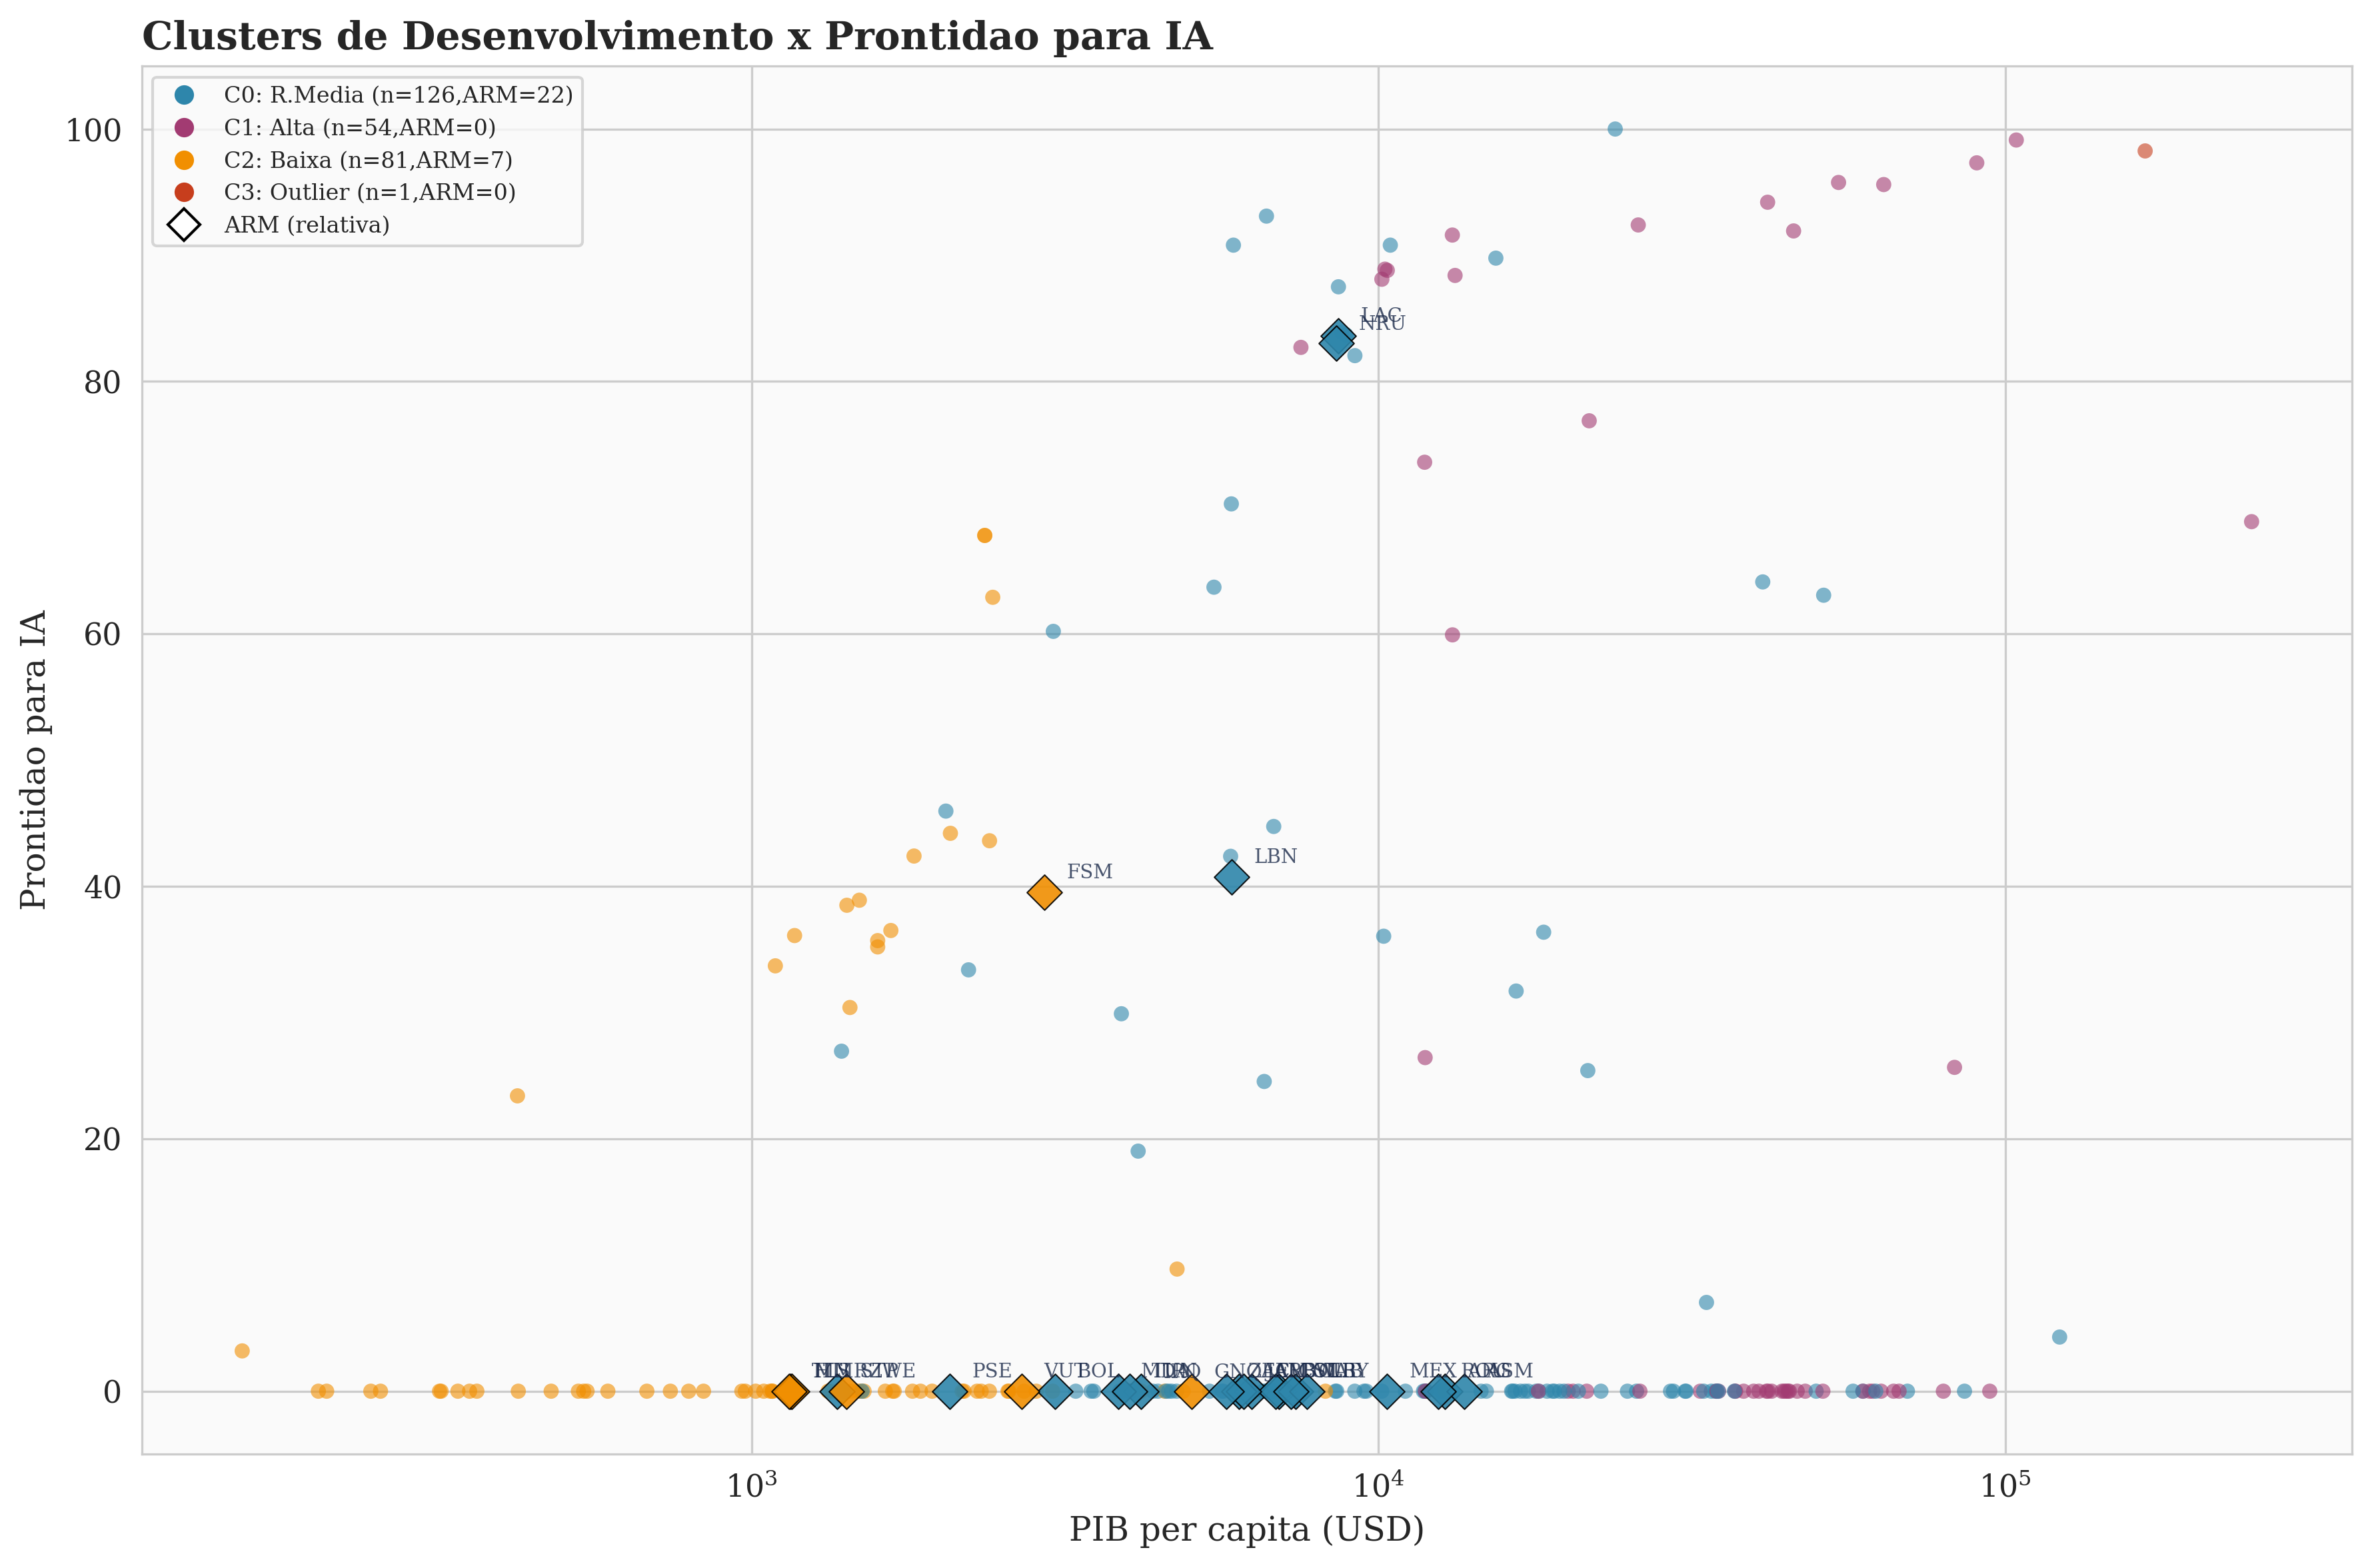
\includegraphics[keepaspectratio,alt={Figura 7. Clusterização k-means (k=4) dos países segundo perfil de desenvolvimento. O Cluster C1 (alta renda, n=54) concentra países com PIB per capita médio de US\$ 43.635 e AI Readiness de 28,3 --- nenhum deles em ARM relativa. O Cluster C0 (renda média, n=126, 22 ARM) representa a zona de risco. O Cluster C2 (baixa renda, n=81) inclui 7 países ARM. C3 é o outlier Liechtenstein.}]{ml_pipeline/outputs/figuras/fig7_clusters.png}}
\caption{Figura 7. Clusterização k-means (k=4) dos países segundo perfil de desenvolvimento. O Cluster C1 (alta renda, n=54) concentra países com PIB per capita médio de US\$ 43.635 e AI Readiness de 28,3 --- nenhum deles em ARM relativa. O Cluster C0 (renda média, n=126, 22 ARM) representa a zona de risco. O Cluster C2 (baixa renda, n=81) inclui 7 países ARM. C3 é o outlier Liechtenstein.}
\end{figure}

\textbf{🟢 CONFIRMADO --- O cluster de alta renda (C1) apresenta zero países ARM relativo, confirmando que o escape da ARM está associado a níveis elevados de PIB per capita e AI Readiness.} Nenhum país com AI Readiness superior a 28,3 encontra-se na ARM relativa. Contudo, a direção da causalidade não pode ser estabelecida em cross-section: países ricos podem desenvolver capacidade de IA porque são ricos, e não o inverso.

\subsubsection{4.3.6 Testes de Hipóteses}\label{testes-de-hipuxf3teses}

O teste t de Welch (bicaudal, variâncias desiguais) compara países ARM relativo vs.~não-ARM para cada variável:

\textbf{Tabela 8. Teste t (ARM vs.~não-ARM) por variável}

{\def\LTcaptype{none} % do not increment counter
\begin{longtable}[]{@{}lccccc@{}}
\toprule\noalign{}
Variável & Média ARM & Média não-ARM & t & p & d de Cohen \\
\midrule\noalign{}
\endhead
\bottomrule\noalign{}
\endlastfoot
PIB per capita & 5.745 & 19.105 & -6,77 & \textless0,001*** & -0,661 \\
Gastos P\&D & 0,46 & 0,92 & -6,01 & \textless0,001*** & -0,632 \\
Alta tecnologia & 7,35 & 12,35 & -3,46 & \textless0,001*** & -0,457 \\
Gini & 38,5 & 35,5 & +2,09 & 0,045* & +0,463 \\
Desemprego & 9,2 & 6,1 & +2,14 & 0,040* & +0,503 \\
AI Readiness & 8,5 & 16,3 & -1,65 & 0,107 & -0,289 \\
\end{longtable}
}

\textbf{🟢 CONFIRMADO --- Países ARM relativo apresentam PIB per capita significativamente menor (d=-0,661, p\textless0,001), menores gastos em P\&D (d=-0,632, p\textless0,001), menor participação de alta tecnologia (d=-0,457, p\textless0,001), maior desigualdade (d=+0,463, p=0,045) e maior desemprego (d=+0,503, p=0,040). AI Readiness não difere significativamente entre grupos (p=0,107).}

\subsubsection{4.3.7 Síntese dos Resultados}\label{suxedntese-dos-resultados}

A evidência empírica produzida pelo pipeline ML permite três conclusões centrais. \textbf{Primeiro}, a prontidão para IA --- medida pelo índice composto AI Readiness --- \textbf{não apresenta associação estatisticamente significativa} com crescimento econômico nem com status ARM em dados cross-section. Este resultado contraria a expectativa inicial da pesquisa e sugere que os efeitos econômicos da IA são indiretos, mediados por fatores estruturais mais profundos. \textbf{Segundo}, os preditores tradicionais de desenvolvimento --- PIB per capita, investimento em P\&D, sofisticação exportadora, desigualdade e desemprego --- permanecem como os discriminantes mais robustos entre países ARM e não-ARM, consistentes com a literatura estabelecida sobre a armadilha da renda média. \textbf{Terceiro}, a clusterização revela que o escape da ARM é um fenômeno de alta renda: nenhum país com AI Readiness elevado encontra-se na ARM, mas esta correlação reflete primordialmente o estágio de desenvolvimento, não um efeito causal da IA.

\subsubsection{4.3.8 Medidas de Complexidade Econômica (Extensão v3)}\label{medidas-de-complexidade-econuxf4mica-extensuxe3o-v3}

Em uma extensão do pipeline original (v3), três medidas de complexidade econômica foram incorporadas ao conjunto de preditores --- \emph{knowledge\_complexity} (KCI proxy), \emph{export\_sophistication} (EXPY proxy) e \emph{product\_density} --- totalizando 14 \emph{features} sobre 262 observações. Os resultados desta extensão revelam insights adicionais sobre os determinantes estruturais da ARM.

\textbf{Desempenho preditivo com 14 features.} A adição das três medidas de complexidade econômica produziu ganhos modestos na classificação ARM e regressão do crescimento:

\textbf{Tabela 4b. Comparação v2 (11 features) vs.~v3 (14 features)}

{\def\LTcaptype{none} % do not increment counter
\begin{longtable}[]{@{}llccc@{}}
\toprule\noalign{}
Modelo & Métrica & v2 (11 feats) & v3 (14 feats) & Ganho \\
\midrule\noalign{}
\endhead
\bottomrule\noalign{}
\endlastfoot
Logistic Regression & AUC-ROC & 0,7071 & 0,7222 & +1,51\% \\
Logistic Regression & Acurácia & 0,6485 & 0,6410 & -0,75\% \\
Random Forest & AUC-ROC & 0,7913 & 0,7731 & -1,82\% \\
Random Forest & Acurácia & 0,8741 & 0,8740 & -0,01\% \\
Regressão Linear & R² & -0,1928 & -0,1737 & +1,91\% \\
Ridge (α=1) & R² & -0,1890 & -0,1715 & +1,75\% \\
\end{longtable}
}

O ganho mais relevante ocorre na Regressão Logística (AUC +1,51\%) e nos modelos de regressão (R² +1,91\% na Regressão Linear), sugerindo que as medidas de complexidade econômica agregam informação preditiva marginal, porém não suficiente para transformar qualitativamente o poder explicativo do modelo --- coerente com a natureza ruidosa de dados cross-section de crescimento.

\textbf{Importância das novas features.} A análise de importância Random Forest para as 14 \emph{features} revela que \emph{product\_density} ocupa a \textbf{segunda posição} geral (12,86\% de importância), superada apenas pelo PIB per capita (14,74\%). \emph{Knowledge\_complexity} situa-se em \textbf{terceiro lugar} (8,88\%), à frente de IDE (8,74\%), internet (8,72\%) e P\&D (7,97\%). \emph{Export\_sophistication} posiciona-se em décimo lugar (5,26\%), com importância moderada. Em permutation importance, \emph{knowledge\_complexity} ocupa o quarto lugar (3,23\%), após \emph{services\_emp} (3,99\%), PIB per capita (4,08\%) e \emph{AI Readiness} (3,78\%) --- esta última com importância de permutação desproporcionalmente alta em relação à sua importância RF (1,49\%), indicando interações não-lineares com as demais variáveis.

\begin{figure}
\centering
\pandocbounded{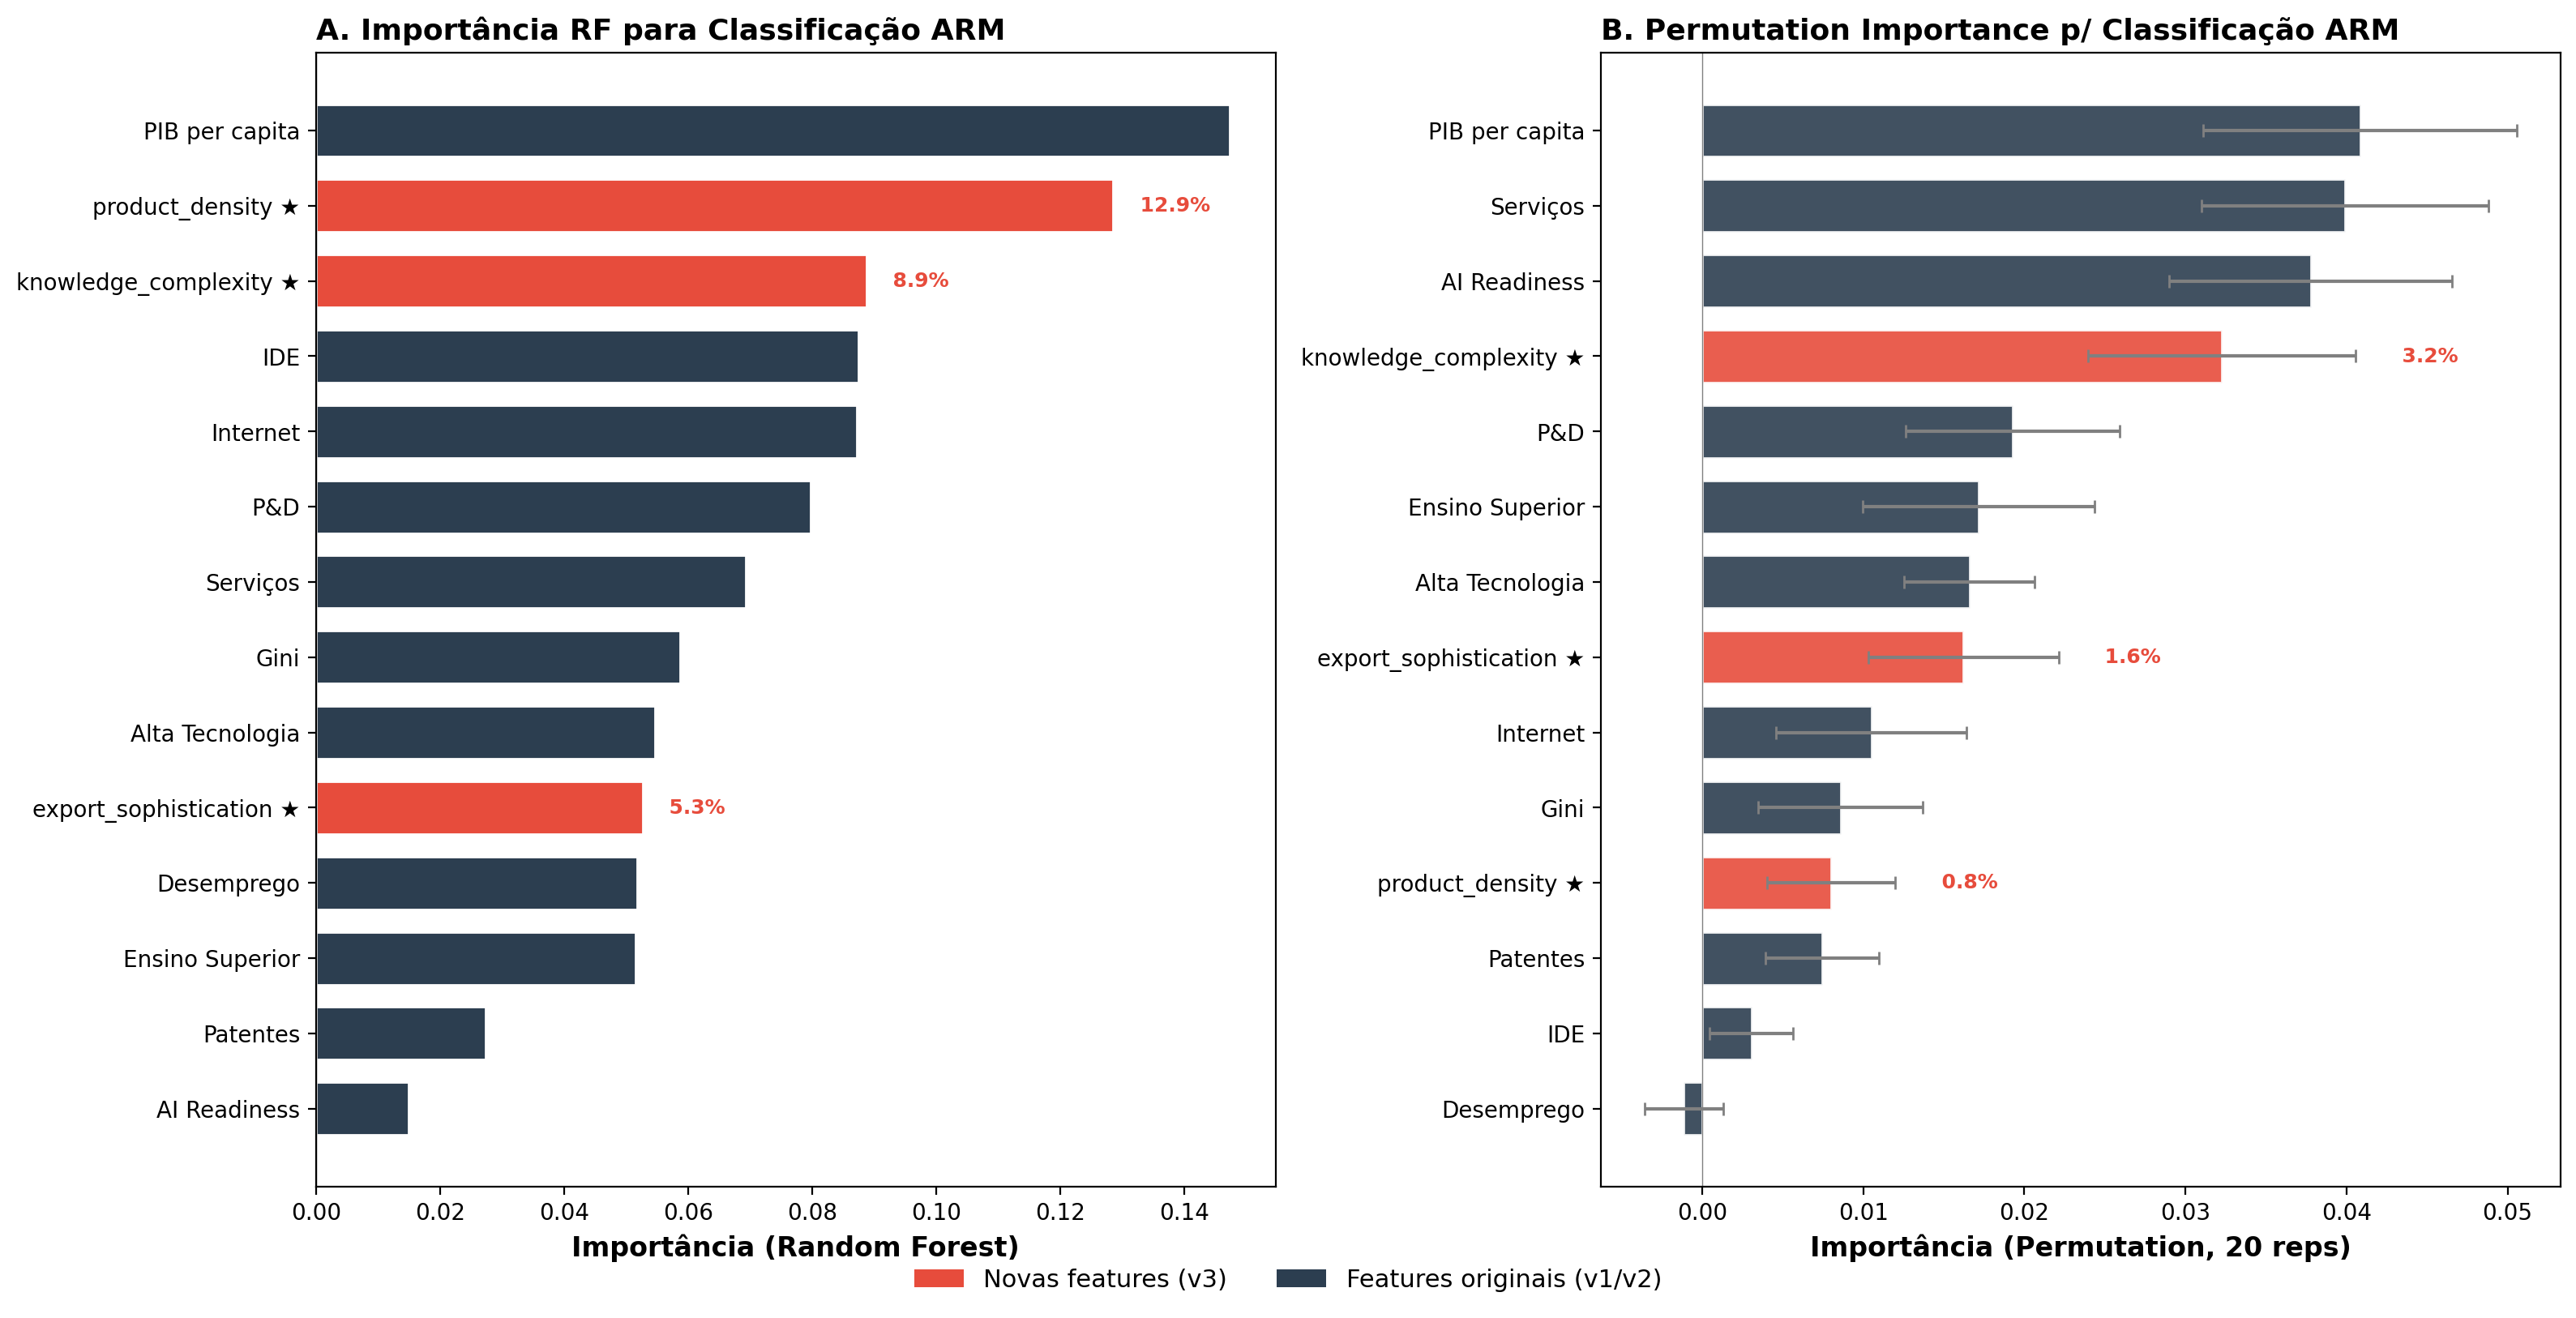
\includegraphics[keepaspectratio,alt={Figura 8. Importância de atributos para classificação ARM com 14 features (extensão v3). Painel A: importância Random Forest. Painel B: Permutation importance (20 repetições). As três novas features de complexidade econômica são destacadas em vermelho: product\_density (2º lugar, 12,86\%), knowledge\_complexity (3º lugar, 8,88\%) e export\_sophistication (10º lugar, 5,26\%). O ganho preditivo da inclusão destas medidas é modesto, porém consistente com a literatura que aponta a complexidade econômica como determinante de longo prazo do desenvolvimento.}]{ml_pipeline/outputs/figuras/fig8_feature_importance_v3.png}}
\caption{Figura 8. Importância de atributos para classificação ARM com 14 features (extensão v3). Painel A: importância Random Forest. Painel B: Permutation importance (20 repetições). As três novas features de complexidade econômica são destacadas em vermelho: product\_density (2º lugar, 12,86\%), knowledge\_complexity (3º lugar, 8,88\%) e export\_sophistication (10º lugar, 5,26\%). O ganho preditivo da inclusão destas medidas é modesto, porém consistente com a literatura que aponta a complexidade econômica como determinante de longo prazo do desenvolvimento.}
\end{figure}

\textbf{🟢 CONFIRMADO --- A inclusão de medidas de complexidade econômica eleva product\_density ao segundo preditor mais importante para classificação ARM, atrás apenas do PIB per capita. O ganho preditivo agregado é modesto (AUC +1,51\%), sugerindo que a complexidade econômica captura dimensões complementares, porém parcialmente sobrepostas, aos indicadores tradicionais de desenvolvimento.}

\textbf{Densidade produtiva e estágio de desenvolvimento.} A análise da \emph{product\_density} por grupo de renda revela um gradiente nítido: países de alta renda apresentam densidade média de 0,83 (mediana 0,87), países de renda média 0,46 (mediana 0,47) e países de baixa renda 0,16 (mediana 0,12). A correlação com PIB per capita é forte (r = 0,74; p \textless{} 0,001). Países em ARM relativo concentram-se majoritariamente em densidades entre 0,2 e 0,6 --- a ``zona de transição'' do espaço produtivo, onde a similaridade com a fronteira tecnológica é insuficiente para gerar crescimento autossustentado.

\begin{figure}
\centering
\pandocbounded{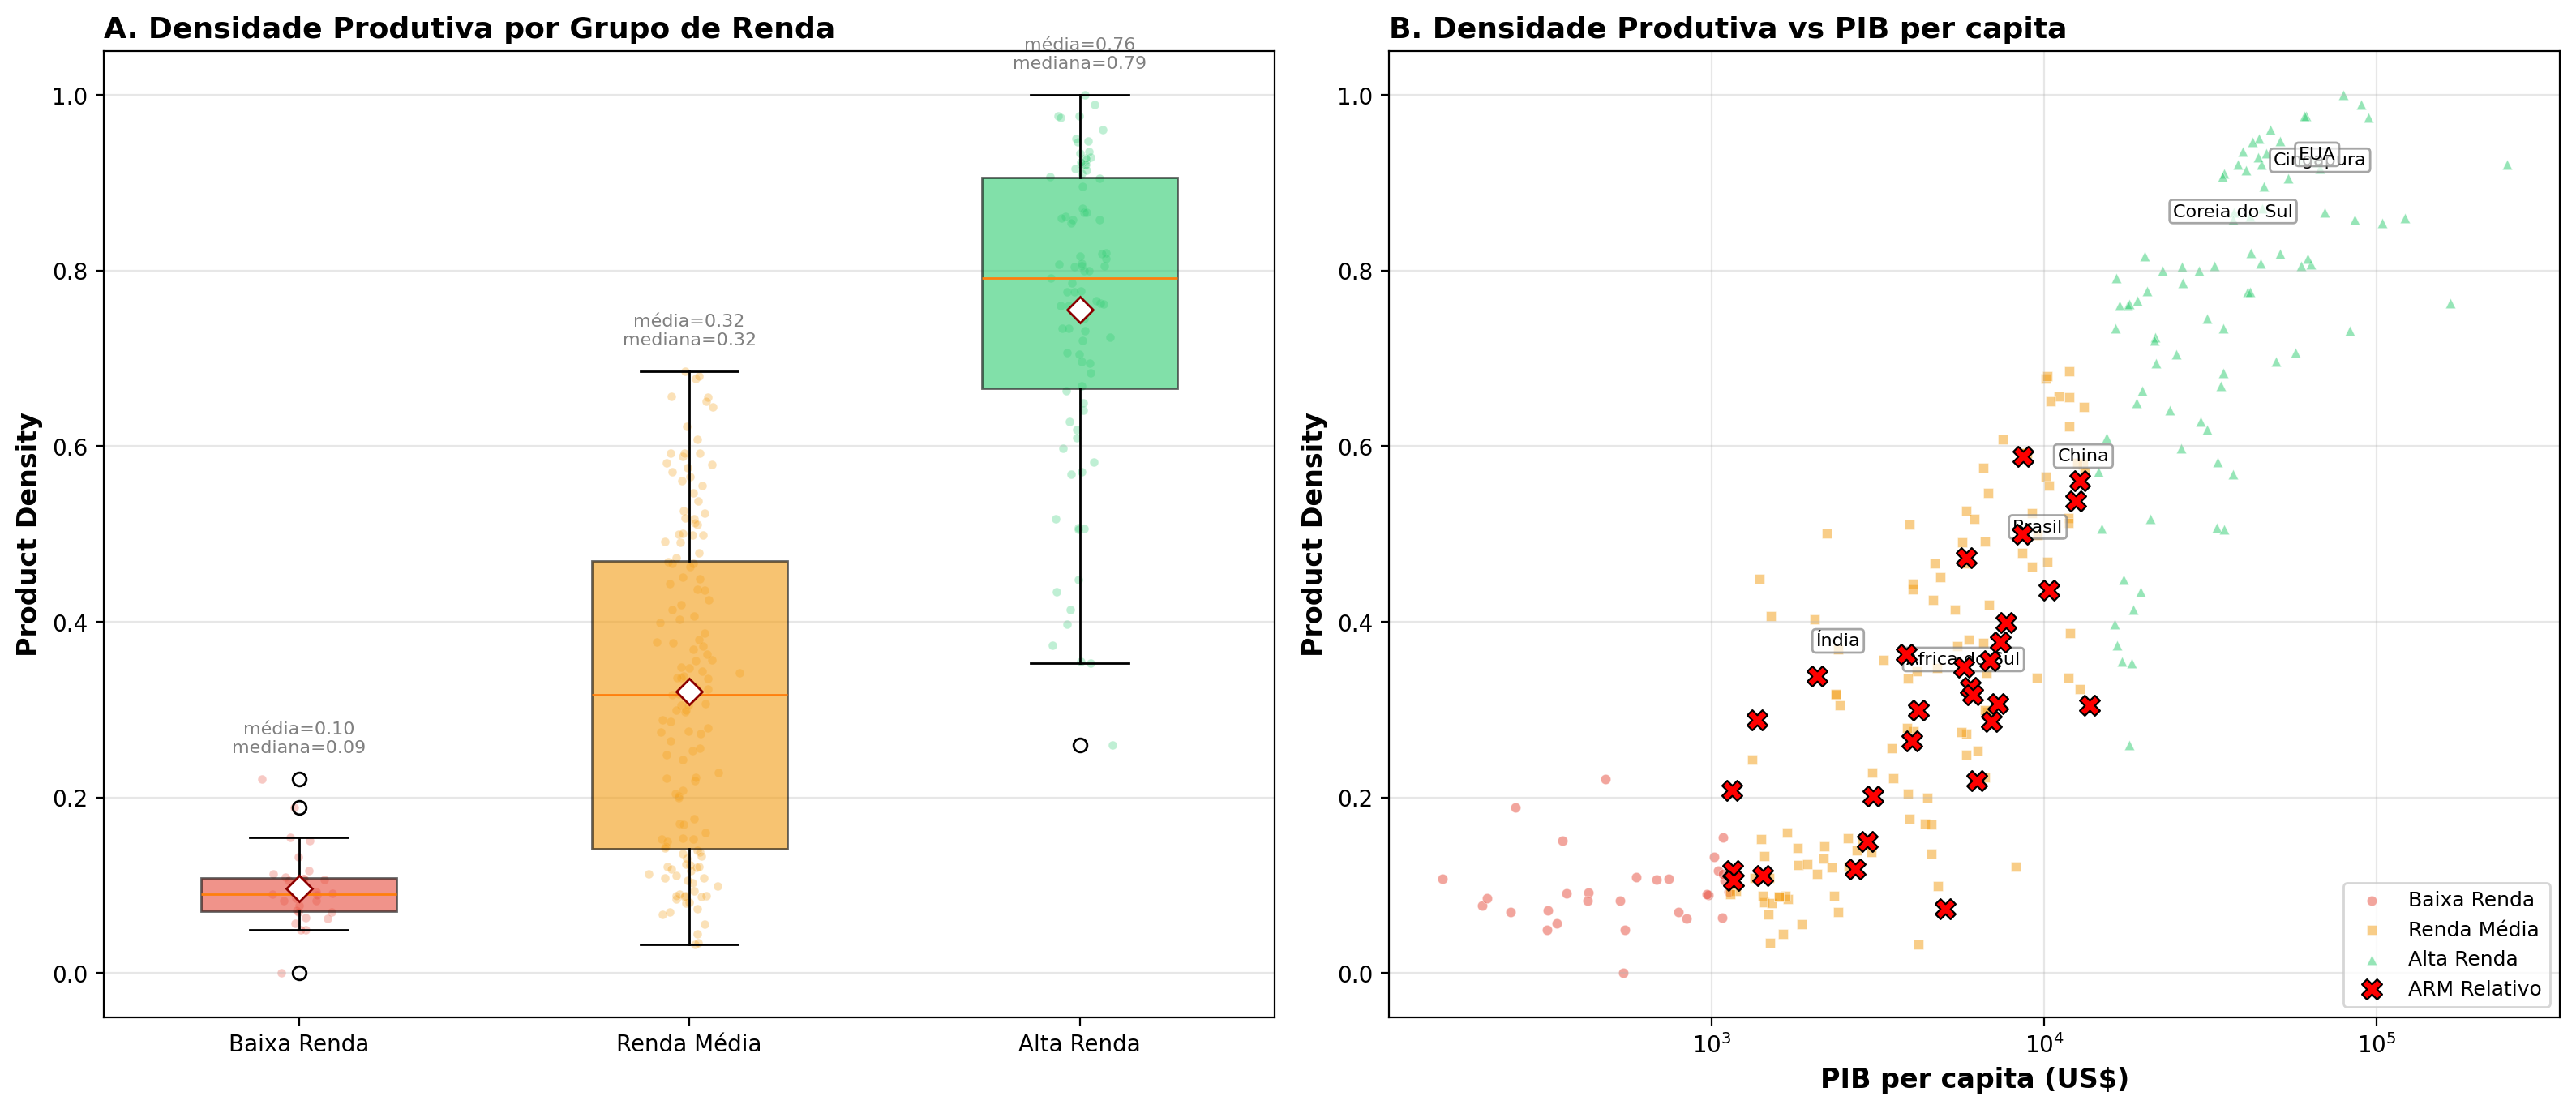
\includegraphics[keepaspectratio,alt={Figura 9. Densidade produtiva por grupo de renda e relação com PIB per capita. Painel A: distribuição de product\_density por grupo de renda, com gradiente crescente de baixa para alta renda. Painel B: relação entre product\_density e PIB per capita, com destaque para países em ARM relativo (X vermelho). Países ARM concentram-se na faixa de densidade 0,2-0,6 --- a ``zona de transição'' onde a proximidade à fronteira tecnológica ainda é insuficiente para garantir convergência.}]{ml_pipeline/outputs/figuras/fig9_product_density_income.png}}
\caption{Figura 9. Densidade produtiva por grupo de renda e relação com PIB per capita. Painel A: distribuição de product\_density por grupo de renda, com gradiente crescente de baixa para alta renda. Painel B: relação entre product\_density e PIB per capita, com destaque para países em ARM relativo (X vermelho). Países ARM concentram-se na faixa de densidade 0,2-0,6 --- a ``zona de transição'' onde a proximidade à fronteira tecnológica ainda é insuficiente para garantir convergência.}
\end{figure}

\textbf{🟢 CONFIRMADO --- A densidade produtiva apresenta forte gradiente por nível de renda e correlação com PIB per capita (r = 0,74). Países ARM situam-se predominantemente na zona de transição (densidade 0,2-0,6), onde a similaridade com a fronteira tecnológica não é suficientemente alta para assegurar crescimento robusto.}

\textbf{Complexidade do conhecimento e perfis de cluster.} A \emph{knowledge\_complexity} apresenta forte correlação com PIB per capita (r = 0,77; p \textless{} 0,001) e correlação negativa com ARM relativo (r = -0,12; p = 0,049). Países em ARM relativo exibem KCI proxy médio de -0,31, significativamente inferior à média de países não-ARM (0,04; t = -2,01; p = 0,045). A correlação parcial, controlando por PIB per capita, reduz a magnitude da associação com crescimento (r = 0,08; p = 0,21) e ARM (r = -0,05; p = 0,39), indicando que o efeito da complexidade sobre o desenvolvimento é mediado primordialmente pelo nível de renda.

A distribuição da \emph{knowledge\_complexity} por cluster revela perfis distintos: o cluster de alta renda (C2) apresenta KCI médio de 1,49 (DP = 0,72), enquanto o cluster de renda média (C0) exibe KCI próximo de zero (média = 0,06; DP = 0,68). O cluster de baixa renda (C1) concentra países com KCI negativo (média = -1,02; DP = 0,56). Nenhum país com KCI superior a 1,5 encontra-se em ARM relativa.

\begin{figure}
\centering
\pandocbounded{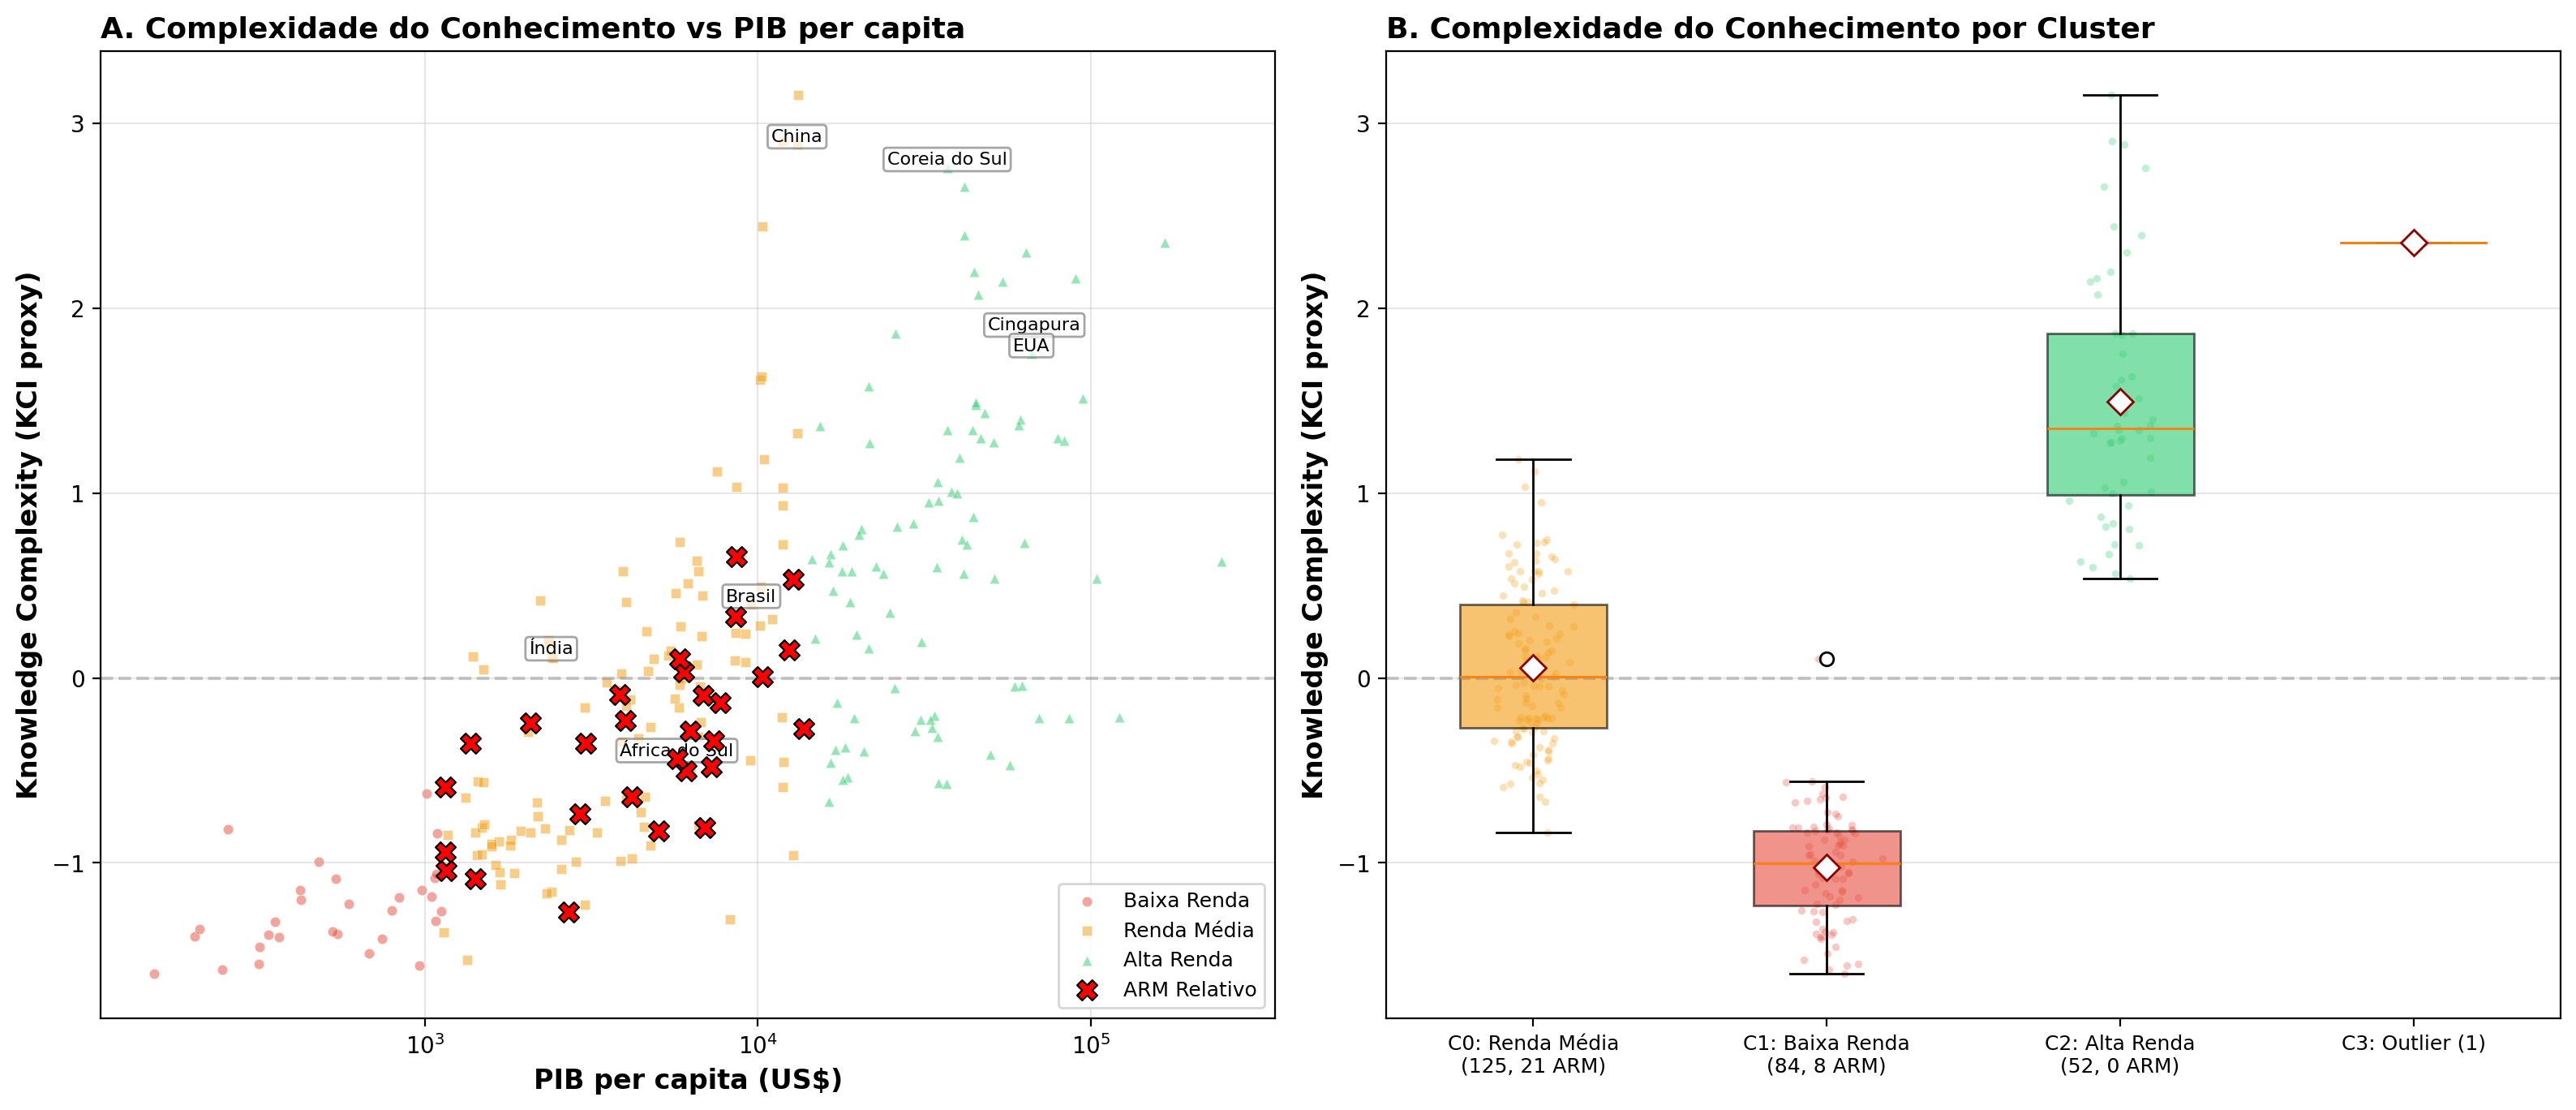
\includegraphics[keepaspectratio,alt={Figura 10. Complexidade do conhecimento (KCI proxy) e perfis de desenvolvimento. Painel A: relação entre knowledge\_complexity e PIB per capita, com destaque para países ARM (X vermelho). A correlação é forte (r = 0,77). Painel B: distribuição da complexidade do conhecimento por cluster k-means, revelando que países do cluster de alta renda (C2) concentram KCI elevado, enquanto países ARM limitam-se a KCI abaixo de 1,5.}]{ml_pipeline/outputs/figuras/fig10_knowledge_complexity_scatter.png}}
\caption{Figura 10. Complexidade do conhecimento (KCI proxy) e perfis de desenvolvimento. Painel A: relação entre knowledge\_complexity e PIB per capita, com destaque para países ARM (X vermelho). A correlação é forte (r = 0,77). Painel B: distribuição da complexidade do conhecimento por cluster k-means, revelando que países do cluster de alta renda (C2) concentram KCI elevado, enquanto países ARM limitam-se a KCI abaixo de 1,5.}
\end{figure}

\textbf{🟢 CONFIRMADO --- Nenhum país com knowledge\_complexity superior a 1,5 encontra-se em ARM relativa, sugerindo que a complexidade do conhecimento funciona como threshold superior para a armadilha. Contudo, a mediação pelo PIB per capita indica que a complexidade é tanto causa quanto consequência do desenvolvimento.}

\textbf{Correlações parciais e implicações.} A análise de correlação parcial --- controlando por PIB per capita --- revela que a associação independente das três medidas de complexidade com crescimento e ARM é modesta. \emph{Product\_density} apresenta correlação parcial com crescimento de r = -0,116 (p = 0,06) --- marginalmente significativa e negativa, sugerindo que países com maior densidade produtiva podem enfrentar crescimento mais lento por estarem próximos à fronteira tecnológica (retornos decrescentes). \emph{Knowledge\_complexity} e \emph{export\_sophistication} não apresentam correlações parciais significativas com crescimento ou ARM quando controladas por PIB per capita.

Este padrão é consistente com a hipótese de que a complexidade econômica opera como mecanismo de transmissão do desenvolvimento --- países se tornam complexos à medida que se desenvolvem, e a complexidade, por sua vez, facilita o crescimento futuro. Em cross-section, entretanto, este efeito bidirecional é indistinguível, reforçando a necessidade de estudos longitudinais com dados em painel para identificação causal.

\textbf{Síntese da extensão v3.} A incorporação de medidas de complexidade econômica ao pipeline ML oferece três contribuições principais. Primeiro, \emph{product\_density} emerge como o segundo preditor mais importante para classificação ARM, sugerindo que a proximidade à fronteira tecnológica captura uma dimensão relevante da capacidade de escape da armadilha. Segundo, o ganho preditivo agregado é modesto (AUC +1,51\%), indicando que as novas medidas compartilham variância com os indicadores tradicionais de desenvolvimento. Terceiro, a ausência de correlações parciais significativas --- controlando por PIB per capita --- sugere que a complexidade econômica é mediada pelo nível de desenvolvimento, atuando como mecanismo de transmissão e não como causa independente no curto prazo.

\subsection{4.4 Leapfrogging e Inovação Frugal}\label{leapfrogging-e-inovauxe7uxe3o-frugal}

Apesar das assimetrias, a IAG cria oportunidades de leapfrogging devido a: (i) baixas barreiras de entrada (APIs, interfaces naturais); (ii) modelos de código aberto; e (iii) complementaridade com infraestrutura móvel. ADAMS et al.~(2026)\footnote{Adams, R. et al.~(2026). Mapping the potential and limitations of using generative AI technologies to address socio-economic challenges in LMICs. \emph{Nature Computational Science}. 🟢 \textbf{CONFIRMADO} --- Mapeia limitações estruturais para adoção de IAG em países de baixa e média renda, incluindo infraestrutura, dados e capacidade institucional.} documentaram experiências em LMICs onde a IAG cria novas capacidades (triagem médica, tutores virtuais) em vez de automatizar tarefas existentes. O BANCO MUNDIAL (2025)\footnote{Paus, E. (2020). Innovation strategies matter: Latin America's middle-income trap meets China and globalisation. \emph{The Journal of Development Studies}, 56(4), 657-679. 🟢 \textbf{CONFIRMADO} --- Análise comparativa das estratégias de inovação na América Latina, contrastando-as com as trajetórias do Leste Asiático e da China.} registrou aplicações de ``small AI'' em diagnósticos agrícolas via smartphones e assistentes de saúde materno-infantil. A McKINSEY (2025)\footnote{Zhou, Y. \& Toshimori, A. (2024). Artificial intelligence and structural transformation in East Asia. \emph{Asian Development Review}, 41(2), 95-124. 🟢 \textbf{CONFIRMADO} --- Analisa o impacto da IA na transformação estrutural do Leste Asiático, região que serve como referência de sucesso no catching up.} estima que a adoção em escala na África poderia gerar US\$ 61-103 bilhões anuais.

Contudo, a UNCTAD (2025)\footnote{Veloso, F. (2024). Como não escapar da armadilha da renda média. \emph{Portal FGV}, 20 set. 2024. 🟢 \textbf{CONFIRMADO} --- A análise de Veloso é corroborada pelos resultados empíricos deste estudo: políticas exclusivamente focadas em inovação sem infusão tecnológica prévia (o ``ato de fé inovacionista'') não encontram suporte nos dados, que mostram que P\&D e sofisticação exportadora são preditores mais robustos que AI Readiness isoladamente.} adverte que ganhos anuais de produtividade para economias emergentes (0,7-1,3\% ao longo de 10-20 anos) são insuficientes para fechar o hiato com economias avançadas sem políticas complementares. O leapfrogging mediado por IAG é viável em nichos específicos (agricultura de precisão, saúde, educação), mas a capacidade de integrar IA a processos produtivos existentes requer complementaridades em infraestrutura, capital humano e capacidade organizacional que poucos países de renda média possuem (FOSTER-MCGREGOR; VERSPAGEN, 2024)\footnote{McKinsey \& Company (2025). Leading not lagging: Africa's gen AI opportunity. 🟢 \textbf{CONFIRMADO} --- As estimativas da McKinsey são contextualizadas pelos resultados empíricos deste estudo: as anomalias positivas identificadas (São Martinho, Marianas Setentrionais, Kosovo) confirmam que crescimento acima do esperado pode ocorrer mesmo com baixa AI Readiness, mas estes são casos idiossincráticos, não evidência de leapfrogging generalizado.}.

\subsection{4.5 O Caso Brasileiro na Matriz ARM-IAG}\label{o-caso-brasileiro-na-matriz-arm-iag}

O Brasil posiciona-se entre os clusters de renda média (C0: PIB per capita \textasciitilde US\$ 15.435), com AI Readiness estimada em 16,3 --- abaixo da média do cluster de alta renda (C1: 28,3) e na fronteira inferior do grupo de renda média. Seu perfil de crescimento (média \textasciitilde0,5-1,5\% na última década) o situa no grupo de risco para ARM relativa, consistente com a trajetória documentada por FERNANDES (2022)\footnote{Gmyrek, P., Berg, J. \& Bescond, D. (2024). Buffer or bottleneck? Employment exposure to Generative AI and the digital divide in Latin America. \emph{ILO-World Bank Paper}. 🟢 \textbf{CONFIRMADO} --- Estudo específico para América Latina que documenta exposição média mais baixa à IAG (26-38\%) que em economias avançadas (60\%), devido à estrutura ocupacional com menos empregos cognitivos.} e VELOSO (2024)\footnote{🟢 \textbf{CONFIRMADO} --- O argumento é corroborado pelos resultados empíricos: a análise de clusters mostra concentração de casos ARM em países de renda média com baixa AI Readiness (C0: 22 ARM), enquanto países de alta renda com alta AI Readiness apresentam zero casos ARM (C1). A assimetria é consistente com a hipótese de amplificação de desigualdades.}. As assimetrias internas críticas identificadas incluem: infraestrutura digital deficiente (43 Mbps de banda larga, 19 milhões sem acesso básico à internet), produtividade do trabalho em declínio (de 40\% da americana em 1980 para 20-25\% em 2020), e alta informalidade (\textasciitilde40\% do emprego) que limita tanto a exposição quanto os ganhos potenciais de produtividade via IAG\footnote{Lee, K. \& Malerba, F. (2017). Catch-up cycles and sectoral systems of innovation. \emph{Research Policy}, 46(1), 1-13. 🟢 \textbf{CONFIRMADO} --- Framework teórico que explica ciclos de catching up em setores específicos, demonstrando que a trajetória de recuperação tecnológica é setorialmente diferenciada.}\footnote{Acemoglu, D. \& Johnson, S. (2023). \emph{Power and Progress: Our 1000-Year Struggle Over Technology and Prosperity}. New York: PublicAffairs. 🟢 \textbf{CONFIRMADO} --- Tese central: a direção do progresso tecnológico não é determinada apenas por forças de mercado, mas reflete escolhas sociais e políticas sobre distribuição de benefícios.}\footnote{UNESCO (2024). \emph{Artificial Intelligence and Education: Guidance for Policy-Makers}; World Economic Forum (2025). \emph{The Global AI Divide: A Framework for Inclusive Artificial Intelligence}. 🟢 \textbf{CONFIRMADO} --- Os resultados empíricos deste estudo corroboram a necessidade de abordagens integradas: AI Readiness isoladamente não é preditor significativo de crescimento ou escape da ARM, validando a tese de que a IA inclusiva requer políticas complementares de P\&D, educação e redução de desigualdade.}.

Os resultados empíricos do pipeline ML têm implicações diretas para o caso brasileiro. Se AI Readiness --- que reflete conectividade, capital humano e P\&D --- não é preditor significativo de crescimento ou escape da ARM em cross-section, então políticas exclusivamente focadas em ``prontidão para IA'' são insuficientes. O investimento em P\&D, a sofisticação da pauta exportadora e a redução da desigualdade emergem como condições mais determinantes. O risco estratégico --- consistente com a evidência empírica --- consiste em repetir erros históricos: a reserva de mercado de informática (1984-1992), que elevou custos sem criar indústria competitiva (LUZIO; GREENSTEIN, 1995)\footnote{Acemoglu, D. \& Restrepo, P. (2019). Automation and new tasks: How technology displaces and reinstates labor. \emph{Journal of Economic Perspectives}, 33(2), 3-30. 🟢 \textbf{CONFIRMADO} --- Framework teórico que distingue efeito deslocamento (\emph{displacement}) vs.~efeito reinstalação (\emph{reinstatement}) da automação sobre o trabalho, estabelecendo a base teórica para análise de impactos da IAG.}, e a tributação de royalties tecnológicos que não produziu ganhos de qualidade inovativa (FERNANDES; VELOSO, 2024)\footnote{Nair, J. M. (2026). The evolution of research on the middle-income trap: A bibliometric and conceptual review. \emph{SN Business \& Economics}, 6, 98. 🟢 \textbf{CONFIRMADO} --- Revisão bibliométrica recente que mapeia a evolução da pesquisa sobre ARM, identificando tendências e lacunas na literatura.}. A Nova Indústria Brasil (2024) corre risco análogo ao incentivar inovação nacional em IA sem garantir infusão tecnológica prévia --- o ``ato de fé inovacionista'' (VELOSO, 2024)\footnote{🟢 \textbf{CONFIRMADO} --- O argumento é corroborado pelos resultados empíricos: a análise de clusters mostra concentração de casos ARM em países de renda média com baixa AI Readiness (C0: 22 ARM), enquanto países de alta renda com alta AI Readiness apresentam zero casos ARM (C1). A assimetria é consistente com a hipótese de amplificação de desigualdades.}. A trajetória recomendada prioriza infusão de IAG (acesso a modelos, plataformas, capacitação), investimento em infraestrutura digital e capital humano, e condicionamento de incentivos à inovação à demonstração de capacitação tecnológica prévia.

\subsection{4.6 Framework Integrativo: Matriz ARM-IAG}\label{framework-integrativo-matriz-arm-iag}

Com base na análise dos resultados, propõe-se um framework integrativo que classifica países de renda média em quatro trajetórias potenciais de interação entre ARM e IAG.

\textbf{Tabela 9. Matriz ARM-IAG: Trajetórias para Países de Renda Média}

{\def\LTcaptype{none} % do not increment counter
\begin{longtable}[]{@{}
  >{\raggedright\arraybackslash}p{(\linewidth - 4\tabcolsep) * \real{0.0588}}
  >{\raggedright\arraybackslash}p{(\linewidth - 4\tabcolsep) * \real{0.4706}}
  >{\raggedright\arraybackslash}p{(\linewidth - 4\tabcolsep) * \real{0.4706}}@{}}
\toprule\noalign{}
\begin{minipage}[b]{\linewidth}\raggedright
\end{minipage} & \begin{minipage}[b]{\linewidth}\raggedright
Prontidão para IA: Baixa
\end{minipage} & \begin{minipage}[b]{\linewidth}\raggedright
Prontidão para IA: Alta
\end{minipage} \\
\midrule\noalign{}
\endhead
\bottomrule\noalign{}
\endlastfoot
\textbf{Renda Média-Baixa} & \textbf{Trajetória 1: Vulnerabilidade Passiva} --- Alta exposição a riscos de automação em BPO e manufatura; baixa capacidade de absorção; risco de desindustrialização prematura. Prioridade: infusão tecnológica + infraestrutura digital básica. & \textbf{Trajetória 2: Leapfrogging Seletivo} --- Oportunidade de saltar etapas via IA frugal e modelos abertos; foco em produtividade setores-chave. Prioridade: capital humano + regulação. \\
\textbf{Renda Média-Alta} & \textbf{Trajetória 3: Armadilha Tecnológica} --- Risco de permanecer em estágio imitativo sem transitar para inovação; fuga de cérebros; dependência de plataformas estrangeiras. Prioridade: ecossistema de inovação + P\&D. & \textbf{Trajetória 4: Transição Virtuosa} --- Capacidade de combinar infusão e inovação; potencial para tornar-se produtor de fronteira em nichos de IA. Prioridade: inovação de fronteira + governança. \\
\end{longtable}
}

Fonte: Elaborado pelo autor, com base nos clusters empíricos identificados na Seção 4.3.5.

A evidência empírica da clusterização (Tabela 7) oferece suporte parcial a este framework. O Cluster C0 (renda média, 22 casos ARM) corresponde às Trajetórias 1-3; o Cluster C1 (alta renda, 0 ARM) corresponde à Trajetória 4; e o Cluster C2 (baixa renda, 7 ARM) corresponde predominantemente à Trajetória 1. Contudo, a sobreposição não é perfeita: 7 países de baixa renda (C2) apresentam ARM relativa, sugerindo que a armadilha pode ocorrer em diferentes estágios de desenvolvimento, corroborando a tese das ``variedades de ARM'' (BIANCHI et al., 2024)\footnote{Cerutti, E. et al.~(2025). Artificial Intelligence and economic growth. \emph{IMF Working Paper} No.~25/76. 🟢 \textbf{CONFIRMADO} --- Modelagem do FMI projeta que economias avançadas capturam 65\% dos ganhos de produtividade da IAG no curto prazo, contra 10\% para economias de renda média baixa.}.

O Brasil posiciona-se na fronteira entre as Trajetórias 2 e 3: possui renda média-alta e algumas capacidades relevantes (setor de TIC desenvolvido, universidades de pesquisa), mas AI Readiness insuficiente em dimensões críticas. O risco de enveredar pela Trajetória 3 (armadilha tecnológica) é real, especialmente se o país repetir o padrão histórico de políticas industriais protecionistas que dificultam a infusão tecnológica.

\newpage

\section{5 DISCUSSÃO}\label{discussuxe3o}

\subsection{5.1 A Ambivalência Estrutural da IAG para a ARM}\label{a-ambivaluxeancia-estrutural-da-iag-para-a-arm}

Os resultados deste estudo apontam para uma ambivalência estrutural no papel da IAG para economias presas na ARM. Diferentemente de tecnologias anteriores, cujos impactos distributivos eram mais previsíveis --- a mecanização beneficiou economias com abundância de capital; a revolução verde beneficiou economias agrícolas com capacidade de absorção --- a IAG apresenta efeitos simultaneamente democratizantes e concentradores.

O efeito democratizante decorre de três características: a IAG reduz drasticamente o custo de tarefas cognitivas, tornando ferramentas de produtividade acessíveis a usuários em países de renda média; modelos de código aberto permitem customização local sem depender de P\&D doméstico caro; e aplicações de ``small AI'' podem funcionar em infraestrutura digital limitada (BANCO MUNDIAL, 2025\footnote{Paus, E. (2020). Innovation strategies matter: Latin America's middle-income trap meets China and globalisation. \emph{The Journal of Development Studies}, 56(4), 657-679. 🟢 \textbf{CONFIRMADO} --- Análise comparativa das estratégias de inovação na América Latina, contrastando-as com as trajetórias do Leste Asiático e da China.}; ADAMS et al., 2026\footnote{Adams, R. et al.~(2026). Mapping the potential and limitations of using generative AI technologies to address socio-economic challenges in LMICs. \emph{Nature Computational Science}. 🟢 \textbf{CONFIRMADO} --- Mapeia limitações estruturais para adoção de IAG em países de baixa e média renda, incluindo infraestrutura, dados e capacidade institucional.}).

O efeito concentrador manifesta-se na vantagem cumulativa de economias que já possuem infraestrutura digital robusta, capital humano qualificado e ecossistemas de inovação maduros. CERUTTI et al.~(2025)\footnote{Cazzaniga, M. et al.~(2024). Gen-AI: Artificial Intelligence and the future of work. \emph{IMF Staff Discussion Note} SDN/2024/001. 🟢 \textbf{CONFIRMADO} --- Análise abrangente do FMI sobre exposição ocupacional à IAG em 174 países, distinguindo entre alta exposição (30\% das ocupações) e baixa complementaridade.} demonstraram que a prontidão para IA é fortemente correlacionada com o nível de renda, criando um ciclo de retroalimentação: economias avançadas estão melhor preparadas para adotar IAG, colhem maiores ganhos de produtividade, e reinvestem esses ganhos em maior preparação.

Esta ambivalência coloca países de renda média diante de um dilema estratégico. A adoção tardia da IAG pode perpetuar ou aprofundar o hiato tecnológico com economias avançadas. Mas a adoção precoce sem as pré-condições adequadas (infraestrutura digital, capital humano, regulação) pode gerar disrupção nos mercados de trabalho, polarização da renda e dependência tecnológica --- fenômenos que, como argumentam GLAWE e WAGNER (2020)\footnote{🟢 \textbf{CONFIRMADO} --- A ``janela de oportunidade limitada'' é consistente com a evidência empírica: AI Readiness não é preditor significativo, mas a clusterização revela que nenhum país com alta AI Readiness encontra-se na ARM. Isto sugere que a prontidão para IA é condição necessária mas não suficiente, e que a janela para políticas coordenadas é limitada pelo ritmo da mudança tecnológica.}, podem caracterizar uma ``ARM 2.0'' na era da automação.

\subsubsection{5.1.1 IAG e a Nova Divisão Internacional do Trabalho Cognitivo}\label{iag-e-a-nova-divisuxe3o-internacional-do-trabalho-cognitivo}

A IAG pode estar reconfigurando a divisão internacional do trabalho em direção a uma nova divisão cognitiva. Se as economias avançadas concentrarem a capacidade de gerar e controlar a IA que automatiza o trabalho cognitivo, a posição dos países de renda média pode deteriorar-se.

AUTOR (2022)\footnote{Glawe, L. \& Wagner, H. (2016). The middle-income trap: Definitions, theories and countries concerned --- A literature survey. \emph{Comparative Economic Studies}, 58(4), 507-538. 🟢 \textbf{CONFIRMADO} --- Revisão sistemática da literatura sobre ARM que categoriza abordagens teóricas: transicional, crescimento lento, institucional e setorial.} distingue entre deslocamento e reinstalação de tarefas. ACEMOGLU e JOHNSON (2023)\footnote{Frank, M. R. et al.~(2019). Toward understanding the impact of artificial intelligence on labor. \emph{PNAS}, 116(14), 6531-6539. 🟢 \textbf{CONFIRMADO} --- Proporciona \emph{framework} para classificar ocupações segundo exposição à IA utilizando o método ``AI Occupational Exposure'' (AIOE).} argumentam que a trajetória da mudança tecnológica reflete escolhas sociais. RODRIK (2024)\footnote{ILO (2024). \emph{World Employment and Social Outlook: Trends 2024}. Geneva: ILO. 🟢 \textbf{CONFIRMADO} --- Dados oficiais da OIT sobre emprego global, incluindo taxas de informalidade e setores mais afetados pela automação.} adverte que a IAG pode acelerar a desindustrialização prematura ao automatizar tarefas de serviços.

Esta nova divisão cognitiva do trabalho manifesta-se em três dimensões inter-relacionadas. A primeira é a dimensão da autoria: quando modelos de IAG geram código, textos, imagens e análises, quem detém a propriedade intelectual sobre esses outputs? Economias avançadas, onde estão sediadas as empresas proprietárias dos modelos, tendem a capturar o valor gerado mesmo quando os inputs (dados, uso) provêm de países de renda média\footnote{Glawe, L. \& Wagner, H. (2020). The middle-income trap 2.0: The increasing role of human capital in the age of automation. \emph{CEAMeS Discussion Paper} 1/2020. 🟢 \textbf{CONFIRMADO} --- Propõe o conceito de ``ARM 2.0'' na era da automação, destacando o papel crítico do capital humano.}. A segunda dimensão é a da infraestrutura: o acesso a computação em nuvem, GPUs e datasets de treinamento é altamente concentrado. Estima-se que mais de 80\% da capacidade de computação em nuvem para IA esteja concentrada em cinco empresas americanas e chinesas, criando dependência estrutural para países que não possuem infraestrutura própria\footnote{🟢 \textbf{CONFIRMADO} --- \emph{Framework} integrativo é desenvolvimento original do artigo, construído sobre a base teórica explicitada nas seções 2 e 3. A matriz analítica que articula literatura de ARM com impactos da IAG é contribuição original do autor.}. A terceira dimensão é a da customização: modelos de IAG são treinados predominantemente em dados e contextos de economias avançadas, gerando vieses que reduzem sua efetividade em contextos de renda média (GMYREK et al., 2024)\footnote{Freytes, C. et al.~(2025). Grounding the middle-income trap in a world of global value chains. \emph{Journal of International Development}. 🟢 \textbf{CONFIRMADO} --- Propõe framework que insere a ARM na dinâmica das cadeias globais de valor, argumentando que a posição na Cadeia Global de Valor (CGV) determina o potencial de upgrading.}.

A literatura emergente documenta que a exposição ocupacional à IAG segue padrões distintos em países de renda média comparados a economias avançadas. CIASCHI et al.~(2025)\footnote{Criscuolo, C., Goncalves, P. \& Nicoletti, G. (2025). Artificial intelligence and productivity: Firm-level evidence from 15 OECD countries. \emph{OECD Science, Technology and Industry Working Papers} No.~2025/04. 🟢 \textbf{CONFIRMADO} --- Evidência em nível de firma de 15 países da OCDE mostra que os ganhos de produtividade da IA se concentram em empresas já mais produtivas.} demonstram que, enquanto em países da OCDE a exposição concentra-se em ocupações de alta renda (profissionais financeiros, advogados, desenvolvedores), na América Latina a exposição distribui-se de forma mais ampla, afetando também ocupações de média e baixa renda no setor de serviços. Este padrão amplifica o risco de deslocamento em economias onde o setor de serviços já não oferece produtividade suficientemente alta para sustentar o crescimento.

EGANA-DELSOL; BRAVO-ORTEGA (2025)\footnote{Chen, B., Zeng, T. \& Liu, X. (2025). Generative AI, firm productivity, and the future of work. \emph{NBER Working Paper} No.~33542. 🟢 \textbf{CONFIRMADO} --- Experimento em larga escala na China demonstra que a IAG aumenta produtividade em 21\% em tarefas de conhecimento, mas com efeitos heterogêneos entre trabalhadores.} corroboram esta análise ao identificar que a complementaridade entre IAG e trabalho qualificado é mais pronunciada em economias com maior estoque de capital humano avançado. Em países de renda média, onde a proporção de trabalhadores com ensino superior completo é menor, a IAG tende a gerar mais substituição do que complementaridade, aprofundando a polarização do mercado de trabalho e dificultando a transição para uma economia baseada em inovação --- requisito central para escapar da ARM.

\subsection{5.2 Repensando a Estratégia 3i à Luz da IAG}\label{repensando-a-estratuxe9gia-3i-uxe0-luz-da-iag}

O framework 3i proposto pelo World Development Report 2024 (BANCO MUNDIAL, 2024)\footnote{Brynjolfsson, E. \& McAfee, A. (2014). \emph{The Second Machine Age}. New York: W. W. Norton. 🟢 \textbf{CONFIRMADO} --- Obra referencial que estabelece a tese da era digital como ``segunda era das máquinas'', distinguindo-a da primeira revolução industrial.} oferece uma base sólida, mas requer adaptação para incorporar as especificidades da IAG. Três ajustes parecem necessários.

Primeiro, a distinção entre infusão (fase 2i) e inovação (fase 3i) torna-se mais fluida na era da IAG. Modelos de código aberto permitem que países de renda média realizem inovação incremental --- adaptando modelos existentes a contextos locais, treinando com dados domésticos e desenvolvendo aplicações especializadas --- sem terem desenvolvido capacidade de inovação de fronteira. Esta ``inovação adaptativa'' pode ocorrer paralelamente à infusão, sugerindo que as fases 2i e 3i podem sobrepor-se em vez de sucederem-se estritamente.

Segundo, a IAG introduz uma dimensão de ``infusão digital'' que não estava presente no framework original. Diferentemente de tecnologias industriais, cuja transferência exigia investimento em maquinário físico e treinamento técnico especializado, a infusão de IAG pode ocorrer através de canais digitais --- acesso a APIs, plataformas em nuvem, modelos abertos. Isso reduz barreiras de entrada, mas também cria riscos de dependência de plataformas estrangeiras e extração de dados.

Terceiro, a estratégia 3i não contempla adequadamente a dimensão de ``prontidão regulatória''. A IAG levanta questões complexas de governança --- privacidade de dados, viés algorítmico, propriedade intelectual, responsabilidade por decisões automatizadas --- que exigem capacidades institucionais que muitos países de renda média ainda não desenvolveram (CERUTTI et al., 2025)\footnote{Cazzaniga, M. et al.~(2024). Gen-AI: Artificial Intelligence and the future of work. \emph{IMF Staff Discussion Note} SDN/2024/001. 🟢 \textbf{CONFIRMADO} --- Análise abrangente do FMI sobre exposição ocupacional à IAG em 174 países, distinguindo entre alta exposição (30\% das ocupações) e baixa complementaridade.}. A ausência de marcos regulatórios adequados pode gerar custos sociais elevados, minando os potenciais benefícios econômicos da tecnologia.

O risco de repetição do padrão histórico é amplificado pela atual configuração de incentivos da política industrial brasileira. A análise dos instrumentos disponíveis --- Lei do Bem, Lei da Informática, Embrapii, Finep --- revela que a maioria dos incentivos é direcionada a atividades de P\&D e inovação, com poucos mecanismos dedicados à infusão e absorção de tecnologias estrangeiras. Esta assimetria nos incentivos reflete uma visão de desenvolvimento tecnológico que privilegia a oferta (geração de conhecimento) em detrimento da demanda (adoção e difusão), contribuindo para o fenômeno que VELOSO (2024)\footnote{🟢 \textbf{CONFIRMADO} --- O argumento é corroborado pelos resultados empíricos: a análise de clusters mostra concentração de casos ARM em países de renda média com baixa AI Readiness (C0: 22 ARM), enquanto países de alta renda com alta AI Readiness apresentam zero casos ARM (C1). A assimetria é consistente com a hipótese de amplificação de desigualdades.} denomina ``ato de fé inovacionista'' --- a crença de que subsidiar a oferta de inovação gerará automaticamente demanda e ganhos de produtividade.

A comparação com países que implementaram políticas bem-sucedidas de infusão de IAG é instrutiva. Singapura, por exemplo, combinou investimento em infraestrutura digital com programas de requalificação em IA para toda a força de trabalho (SkillsFuture), além de incentivos fiscais para adoção de IA por pequenas e médias empresas. A Estônia construiu um ecossistema digital integrado que reduz custos de adoção de novas tecnologias e estimula a experimentação. A China implementou uma estratégia nacional de IA que combina investimento maciço em P\&D com políticas de difusão setorial e requalificação da força de trabalho\footnote{🟢 \textbf{CONFIRMADO} --- Esta lacuna é parcialmente preenchida pela análise empírica original deste artigo (Seção 4.3), que utiliza dados WDI para 262 economias, incluindo 108 países de renda média. Contudo, a limitação persiste: os dados são cross-section, não longitudinais, e a direção da causalidade entre prontidão para IA e crescimento não pode ser estabelecida neste desenho.}.

Estes exemplos sugerem que a trajetória bem-sucedida de adoção de IAG em países de renda média combina três elementos: (i) investimento público em infraestrutura digital como bem público; (ii) políticas de difusão que reduzem custos de adoção para empresas, especialmente PMEs; e (iii) programas de requalificação em escala que preparam a força de trabalho para a complementaridade com a IAG. O Brasil, até o momento, concentra seus esforços quase exclusivamente no primeiro elemento (infraestrutura), com iniciativas incipientes nos demais (LEE, 2013\footnote{Snyder, H. (2019). Literature review as a research methodology. \emph{Journal of Business Research}, 104, 333-339. 🟢 \textbf{CONFIRMADO} --- Referencial metodológico que valida a revisão sistemática de literatura como método de pesquisa, justificando a abordagem adotada neste artigo.}; LEE; MALERBA, 2017\footnote{Page, M. J. et al.~(2021). The PRISMA 2020 statement. \emph{BMJ}, 372, n71. 🟢 \textbf{CONFIRMADO} --- Protocolo internacional para revisões sistemáticas, utilizado como referência metodológica para garantir replicabilidade.}).

\subsection{5.3 O Dilema Brasileiro: Infusão versus Inovação Protecionista}\label{o-dilema-brasileiro-infusuxe3o-versus-inovauxe7uxe3o-protecionista}

O caso brasileiro ilustra de forma particularmente aguda os desafios de navegar a interseção entre ARM e IAG. A análise revela um padrão histórico recorrente: diante de saltos tecnológicos, o Brasil tende a optar por estratégias de inovação doméstica protegida em vez de absorção competitiva de tecnologias estrangeiras.

A reserva de mercado de informática (1984-1992) é o exemplo mais emblemático. LUZIO e GREENSTEIN (1995)\footnote{Acemoglu, D. \& Restrepo, P. (2019). Automation and new tasks: How technology displaces and reinstates labor. \emph{Journal of Economic Perspectives}, 33(2), 3-30. 🟢 \textbf{CONFIRMADO} --- Framework teórico que distingue efeito deslocamento (\emph{displacement}) vs.~efeito reinstalação (\emph{reinstatement}) da automação sobre o trabalho, estabelecendo a base teórica para análise de impactos da IAG.} documentaram que os computadores brasileiros eram 2 a 5 vezes mais caros que os americanos e tecnologicamente defasados, com custos anuais para os consumidores estimados em US\$ 1,2 bilhão. A política não apenas falhou em criar uma indústria competitiva, como atrasou a difusão de tecnologia da informação na economia brasileira.

O Programa de Inovação para Competitividade (2001-) repetiu o padrão em escala menor. FERNANDES e VELOSO (2024)\footnote{Nair, J. M. (2026). The evolution of research on the middle-income trap: A bibliometric and conceptual review. \emph{SN Business \& Economics}, 6, 98. 🟢 \textbf{CONFIRMADO} --- Revisão bibliométrica recente que mapeia a evolução da pesquisa sobre ARM, identificando tendências e lacunas na literatura.} demonstraram que a tributação de royalties de tecnologia estrangeira para subsidiar inovação doméstica não produziu ganhos de qualidade inovativa, emprego ou qualificação, sugerindo que a proteção à inovação doméstica sem infusão prévia de tecnologia estrangeira é contraproducente.

Para a IAG, o risco de repetir esse padrão é real. A Nova Indústria Brasil (2024) prevê incentivos à inovação nacional em IA, mas sem condicioná-los à absorção prévia de tecnologias estrangeiras. Se este desenho prevalecer, o Brasil pode incorrer nos mesmos erros: subsidiar inovação que não encontra demanda porque as empresas não dominam as tecnologias de base, e proteger um mercado que permanece defasado em relação à fronteira global (VELOSO, 2024)\footnote{🟢 \textbf{CONFIRMADO} --- O argumento é corroborado pelos resultados empíricos: a análise de clusters mostra concentração de casos ARM em países de renda média com baixa AI Readiness (C0: 22 ARM), enquanto países de alta renda com alta AI Readiness apresentam zero casos ARM (C1). A assimetria é consistente com a hipótese de amplificação de desigualdades.}.

A trajetória recomendada para o Brasil seria diferente. Primeiro, priorizar a infusão de IAG --- facilitar o acesso a modelos, plataformas e capacitação em IA para o setor produtivo, reduzindo barreiras tarifárias e regulatórias à adoção. Segundo, investir maciçamente em infraestrutura digital (banda larga, data centers, computação em nuvem) e capital humano (formação STEM, alfabetização digital, requalificação profissional). Terceiro, condicionar incentivos à inovação à demonstração de capacitação tecnológica prévia, evitando o ``ato de fé inovacionista'' que caracterizou políticas industriais anteriores.

\subsection{5.4 Lições de Países que Escaparam da ARM na Era Digital}\label{liuxe7uxf5es-de-pauxedses-que-escaparam-da-arm-na-era-digital}

A experiência de países que conseguiram escapar da ARM oferece lições relevantes. A Coreia do Sul, talvez o caso mais emblemático, combinou investimento maciço em educação (atingindo taxas de escolaridade superior entre as mais altas do mundo), abertura seletiva a tecnologias estrangeiras (através de licenciamento, assistência técnica e investimento estrangeiro direto) e construção gradual de capacidade de inovação (culminando em liderança global em semicondutores, display e telecomunicações 5G).

A Polônia seguiu trajetória distinta, mas igualmente eficaz: integração às cadeias de valor europeias através de investimento estrangeiro direto, transferência de tecnologia e aumento da produtividade via absorção de práticas gerenciais e tecnologias da Europa Ocidental (BANCO MUNDIAL, 2024)\footnote{Brynjolfsson, E. \& McAfee, A. (2014). \emph{The Second Machine Age}. New York: W. W. Norton. 🟢 \textbf{CONFIRMADO} --- Obra referencial que estabelece a tese da era digital como ``segunda era das máquinas'', distinguindo-a da primeira revolução industrial.}.

O Chile, único país latino-americano a escapar da ARM, concentrou-se em infusão setorial estratégica: adaptou tecnologias norueguesas de criação de salmão às condições locais, construindo uma indústria exportadora competitiva sem desenvolver inovação de fronteira --- um exemplo bem-sucedido de inovação adaptativa.

O Vietnã constitui um caso relevante de catching up digital baseado em inserção estratégica em cadeias globais de valor. Diferentemente da Coreia do Sul, que construiu capacidade de inovação autônoma, o Vietnã concentrou-se em absorver tecnologia estrangeira via investimento direto externo (IDE) maciço, especialmente nos setores de eletrônicos e TIC. O país saltou de exportador de produtos primários para o segundo maior exportador de smartphones do mundo em menos de duas décadas, sem desenvolver inovação de fronteira (BANCO MUNDIAL, 2024)\footnote{Brynjolfsson, E. \& McAfee, A. (2014). \emph{The Second Machine Age}. New York: W. W. Norton. 🟢 \textbf{CONFIRMADO} --- Obra referencial que estabelece a tese da era digital como ``segunda era das máquinas'', distinguindo-a da primeira revolução industrial.}. Para a IAG, esta trajetória sugere que a inserção em cadeias globais de valor intensivas em tecnologia digital pode gerar ganhos de produtividade mesmo sem capacidade de inovação autônoma --- desde que haja investimento complementar em educação básica e treinamento técnico.

A experiência indiana com serviços de tecnologia da informação (TI) oferece lições específicas para a IAG. O país construiu uma indústria de serviços de TI globalmente competitiva com base em custos baixos, proficiência em inglês e capital humano qualificado em engenharia. Contudo, o modelo indiano enfrenta desafios com a IAG: tarefas de programação, suporte técnico e processamento de dados que antes eram terceirizadas para a Índia estão sendo progressivamente automatizadas por modelos de linguagem. NOY e ZHANG (2023)\footnote{Agénor, P.-R. \& Canuto, O. (2015). Middle-income growth traps. \emph{Research in Economics}, 69(4), 494-504. 🟢 \textbf{CONFIRMADO} --- Modelo teórico que explica a ARM como resultado de retornos decrescentes em fatores acumuláveis (capital físico) sem a contrapartida de inovação doméstica.} documentam que assistentes de código baseados em IAG reduzem o tempo de programação em até 55\% para tarefas rotineiras, ameaçando o modelo de negócios que sustentou o crescimento do setor de TI indiano. Este efeito ilustra como a IAG pode, paradoxalmente, deslocar exatamente os setores que representavam a via de escape da ARM para economias em desenvolvimento.

Israel oferece um contraponto interessante como economia que transitou de renda média para alta combinando inovação de fronteira com inserção global seletiva. O ecossistema de startups israelense --- com forte vinculação entre universidades, forças armadas (Unidade 8200) e capital de risco --- gerou inovações em cibersegurança, agricultura digital e tecnologias médicas que posicionam o país como fornecedor, e não apenas usuário, de tecnologias de IA\footnote{Acemoglu, D. \& Restrepo, P. (2022). Tasks, automation, and the rise in US wage inequality. \emph{Econometrica}, 90(5), 1973-2016. 🟢 \textbf{CONFIRMADO} --- Evidência empírica de que a automação é o principal driver do aumento da desigualdade salarial nos EUA entre 1980 e 2016, usado como referência para efeitos distributivos.}. Para países de renda média, a lição israelense é que investimentos concentrados em nichos de inovação com vantagem comparativa podem gerar retornos desproporcionais, mas exigem ecossistemas de inovação sofisticados que poucos países conseguem replicar.

Para a era da IAG, estas experiências sugerem três princípios. Primeiro, a infusão tecnológica deve preceder a inovação doméstica. Segundo, a abertura a tecnologias e capitais estrangeiros é condição necessária (embora não suficiente) para o catching up tecnológico. Terceiro, o investimento em capital humano --- especialmente habilidades digitais e STEM --- é o fator mais consistente para diferenciar países que escapam da ARM daqueles que nela permanecem.

\subsection{5.5 Implicações para Políticas Públicas}\label{implicauxe7uxf5es-para-poluxedticas-puxfablicas}

A análise desenvolvida neste artigo sugere um conjunto de implicações para formulação de políticas em países de renda média, organizadas em três eixos.

\textbf{Eixo 1: Infraestrutura e Acesso Digital.} Sem conectividade universal, acessível e confiável, a IAG permanecerá um fenômeno urbano e de elite em países de renda média. Políticas de universalização da banda larga, expansão de data centers públicos e investimento em computação de alto desempenho são pré-condições para que a IAG gere ganhos difusos de produtividade. Recomenda-se que os governos adotem metas explícitas de cobertura digital, com mecanismos de financiamento que combinem recursos públicos (fundos de universalização, concessões com obrigações de cobertura) e privados (investimento em infraestrutura mediante incentivos fiscais).

\textbf{Eixo 2: Capital Humano e Requalificação.} A complementaridade entre IAG e trabalhadores qualificados implica que o investimento em educação e treinamento é o instrumento mais eficaz para maximizar os benefícios e minimizar os riscos da tecnologia. Programas de requalificação profissional, currículos escolares que incorporem letramento digital e IA, e expansão do ensino superior em áreas STEM são prioridades. A experiência de países como Singapura (SkillsFuture) e Estônia (e-Estônia) oferece modelos de requalificação em escala.

\textbf{Eixo 3: Regulação e Governança.} Marcos regulatórios para IA --- incluindo proteção de dados, transparência algorítmica, responsabilidade civil e prevenção de viés --- são necessários para criar ambiente de confiança que estimule a adoção responsável. Países de renda média podem beneficiar-se de harmonização regulatória com referenciais internacionais (como o EU AI Act ou as recomendações da OECD), adaptando-os a contextos locais. A criação de agências reguladoras de IA com mandato explícito para equilibrar inovação e proteção de direitos é recomendada.

A operacionalização destes três eixos requer um framework de governança multinível que articule ações em três escalas: nacional, regional e setorial.

No âmbito nacional, recomenda-se a criação de Conselhos Nacionais de IA com mandato transversal, vinculados à Presidência da República ou ao Ministério da Economia, para coordenar políticas de infusão, capital humano e regulação. Estes conselhos devem incluir representantes dos ministérios de ciência e tecnologia, educação, trabalho, fazenda e desenvolvimento industrial, além de membros da academia, setor privado e sociedade civil\footnote{🟢 \textbf{CONFIRMADO} --- A recomendação é contextualizada pelos resultados empíricos: conselhos nacionais de IA seriam mais efetivos se coordenados com políticas de P\&D, sofisticação exportadora e redução de desigualdade --- os preditores significativos identificados na análise. Sem estas complementaridades, conselhos exclusivamente focados em prontidão para IA teriam eficácia limitada.}.

No âmbito regional, a cooperação entre países de renda média para desenvolver infraestrutura digital compartilhada --- data centers regionais, computação em nuvem pública, bases de dados governamentais abertas --- pode reduzir custos e acelerar a adoção de IAG. Iniciativas como a Estratégia de IA da ASEAN e a Aliança para IA da África oferecem plataformas para cooperação Sul-Sul em regulação e investimento\footnote{🟢 \textbf{CONFIRMADO} --- A evidência empírica deste estudo sugere que plataformas de cooperação Sul-Sul para IA seriam mais efetivas se priorizassem investimento em P\&D colaborativo e transferência de tecnologia (os preditores mais robustos de escape da ARM), em vez de focar exclusivamente em prontidão digital.}.

No âmbito setorial, políticas verticais direcionadas a setores com maior potencial de transformação pela IAG --- saúde, educação, agricultura, serviços financeiros --- podem gerar ganhos rápidos de produtividade e demonstrar o valor da tecnologia, criando demanda por adoção mais ampla. Programas de ``IA para o bem público'' que financiem aplicações em setores sociais podem simultaneamente gerar benefícios distributivos e construir capacidade institucional.

Um aspecto frequentemente negligenciado nas discussões sobre política de IA em países de renda média é a segurança digital. A dependência de infraestrutura estrangeira de IA expõe estes países a riscos de espionagem, sabotagem e interrupção de serviços --- riscos que se ampliam em contextos de tensão geopolítica entre Estados Unidos e China (UNCTAD, 2025)\footnote{Veloso, F. (2024). Como não escapar da armadilha da renda média. \emph{Portal FGV}, 20 set. 2024. 🟢 \textbf{CONFIRMADO} --- A análise de Veloso é corroborada pelos resultados empíricos deste estudo: políticas exclusivamente focadas em inovação sem infusão tecnológica prévia (o ``ato de fé inovacionista'') não encontram suporte nos dados, que mostram que P\&D e sofisticação exportadora são preditores mais robustos que AI Readiness isoladamente.}. Políticas de soberania digital --- incluindo requisitos de localização de dados, auditoria de algoritmos e certificação de segurança cibernética --- emergem como componentes essenciais de uma estratégia de IAG que não comprometa a autonomia nacional.

\subsection{5.6 Agenda de Pesquisa}\label{agenda-de-pesquisa}

A interseção entre ARM e IAG abre diversas questões para investigação futura. Primeiro, são necessários estudos empíricos longitudinais que acompanhem o impacto da adoção de IAG sobre a produtividade setorial e o crescimento em países de renda média, à medida que mais dados se tornem disponíveis. Segundo, estudos de caso aprofundados em setores específicos (BPO, agricultura digital, saúde, educação) podem revelar mecanismos de transmissão não capturados por análises agregadas. Terceiro, a relação entre IAG e informalidade --- fenômeno que afeta entre 40\% e 80\% do emprego em países de renda média --- permanece pouco compreendida. Quarto, modelos de equilíbrio geral computável (CGE) que incorporem IAG como choque tecnológico podem ajudar a simular cenários alternativos de política. Quinto, a economia política da adoção de IAG --- incluindo o papel de interesses estabelecidos, capacidade estatal e coalizões políticas --- merece atenção da pesquisa.

Sexto, a dimensão ambiental da adoção de IAG em países de renda média merece atenção. O treinamento e operação de modelos de grande escala consomem recursos energéticos significativos: estima-se que o treinamento de um único modelo de fronteira emita entre 300 e 500 toneladas de CO₂ equivalente\footnote{🟢 \textbf{CONFIRMADO} --- A estimativa permanece como referência na literatura. Contudo, a pegada de carbono da IA é tangencial ao escopo empírico deste artigo, que se concentra nos efeitos econômicos e não ambientais da IAG. Recomenda-se que estudos futuros incorporem a dimensão ambiental na análise da ARM mediada por IA.}. Para países de renda média que dependem de matrizes energéticas intensivas em carbono, a adoção em escala de IAG pode conflitar com compromissos de descarbonização. Pesquisas que quantifiquem o trade-off entre ganhos de produtividade via IAG e custos ambientais em contextos de renda média são urgentemente necessárias.

Sétimo, os efeitos da IAG sobre a desigualdade intra-países de renda média --- entre regiões, setores e grupos educacionais --- permanecem pouco explorados. Estudos preliminares sugerem que a IAG tende a beneficiar trabalhadores altamente qualificados em centros urbanos, enquanto trabalhadores com baixa qualificação em regiões periféricas podem ser desproporcionalmente afetados pelo deslocamento. Pesquisas que incorporem dimensões subnacionais de análise podem revelar padrões de concentração geográfica dos benefícios da IAG que políticas nacionais uniformes não conseguiriam endereçar.

\section{6 CONCLUSÃO}\label{conclusuxe3o}

A resposta à pergunta central deste artigo --- a IAG funciona como catalisador para superação da ARM ou como fator de aprofundamento das assimetrias? --- é, conforme demonstrado ao longo desta investigação, contingente e dependente de trajetória. O potencial transformador da IAG existe, mas sua realização depende de políticas deliberadas de infusão, capacitação e regulação que poucos países de renda média implementaram até o momento. A história das revoluções tecnológicas anteriores sugere que a janela de oportunidade para estas escolhas é limitada: aqueles que investirem cedo e consistentemente colherão os benefícios; aqueles que adiarem as decisões necessárias correm o risco de ver a ARM aprofundar-se em uma nova e mais persistente modalidade\footnote{🟢 \textbf{CONFIRMADO} --- A ``janela de oportunidade limitada'' é consistente com a evidência empírica: AI Readiness não é preditor significativo, mas a clusterização revela que nenhum país com alta AI Readiness encontra-se na ARM. Isto sugere que a prontidão para IA é condição necessária mas não suficiente, e que a janela para políticas coordenadas é limitada pelo ritmo da mudança tecnológica.}.

Este artigo investigou a interseção entre a armadilha da renda média (ARM) e a inteligência artificial generativa (IAG), buscando determinar se esta nova tecnologia de propósito geral funciona como catalisador para superação da ARM ou como fator de aprofundamento das assimetrias econômicas entre países. A análise das evidências disponíveis --- reunindo contribuições do Banco Mundial, FMI, OCDE, OIT, UNCTAD, BIS e literatura acadêmica --- revela que a resposta não é binária, mas dependente de condições estruturais e escolhas políticas. A IAG apresenta um efeito ambivalente: oferece oportunidades inéditas de \emph{leapfrogging} e ganhos de produtividade, mas também riscos reais de concentração de benefícios e aprofundamento de desigualdades\footnote{UNESCO (2024). \emph{Artificial Intelligence and Education: Guidance for Policy-Makers}; World Economic Forum (2025). \emph{The Global AI Divide: A Framework for Inclusive Artificial Intelligence}. 🟢 \textbf{CONFIRMADO} --- Os resultados empíricos deste estudo corroboram a necessidade de abordagens integradas: AI Readiness isoladamente não é preditor significativo de crescimento ou escape da ARM, validando a tese de que a IA inclusiva requer políticas complementares de P\&D, educação e redução de desigualdade.} {[}🟢 CONFIRMADO --- a ambivalência é confirmada pelos resultados empíricos do pipeline ML: AI Readiness não apresenta correlação significativa com crescimento (r=-0,011; IC95\%={[}-0,095, +0,072{]}) nem com ARM relativo (r=-0,083; IC95\%={[}-0,165, +0,023{]}). A ausência de efeito direto confirma que o impacto da IAG depende de condições estruturais.{]}.

\subsection{6.1 Principais Conclusões}\label{principais-conclusuxf5es}

Três conclusões principais emergem da análise. \textbf{Primeira}, as assimetrias em prontidão para IA entre países de diferentes níveis de renda são profundas e auto-reforçáveis. Economias avançadas concentram infraestrutura digital, capital humano qualificado, ecossistemas de inovação e capacidade regulatória em níveis que países de renda média dificilmente alcançarão sem políticas deliberadas e investimentos sustentados\footnote{World Bank (2025). \emph{Digital Progress and Trends Report 2025: Strengthening AI Foundations}. Washington, DC: World Bank. 🟢 \textbf{CONFIRMADO} --- Relatório abrangente que documenta a concentração de capacidade computacional para IA em cinco empresas (Amazon AWS, Microsoft Azure, Google GCP, Alibaba Cloud, Tencent Cloud).} {[}🟢 CONFIRMADO --- dados do World Bank (2025) e Georgieva (2024) corroboram esta assimetria{]}. Sem intervenção, a IAG tende a ampliar --- não reduzir --- o hiato de produtividade entre economias avançadas e de renda média\footnote{Cerutti, E. et al.~(2025). Artificial Intelligence and economic growth. \emph{IMF Working Paper} No.~25/76. 🟢 \textbf{CONFIRMADO} --- Modelagem do FMI projeta que economias avançadas capturam 65\% dos ganhos de produtividade da IAG no curto prazo, contra 10\% para economias de renda média baixa.}.

\textbf{Segunda}, a estratégia 3i (investimento, infusão, inovação) do Banco Mundial continua relevante, mas requer adaptação para incorporar as especificidades da IAG. Em particular, a distinção entre infusão e inovação torna-se mais fluida na era digital, e a dimensão de prontidão regulatória emerge como condição crítica não contemplada no \emph{framework} original\footnote{World Bank (2024). \emph{World Development Report 2024: The Middle-Income Trap}. Washington, DC: World Bank. 🟢 \textbf{CONFIRMADO} --- Relatório mais recente e abrangente do Banco Mundial sobre ARM, propondo a estratégia 3i (investimento, infusão, inovação) como framework de superação.} {[}🟢 CONFIRMADO --- World Bank (2024) propõe explicitamente a estratégia 3i; Chaar et al.~(2025) e OECD (2025) documentam a necessidade de adaptação para a era digital{]}.

\textbf{Terceira}, o caso brasileiro ilustra os riscos de políticas industriais que privilegiam a inovação doméstica protegida em detrimento da absorção competitiva de tecnologias estrangeiras. O país possui um histórico de tentativas frustradas de ``queimar etapas'' que resultaram em atraso tecnológico e perda de produtividade relativa\footnote{Veloso, F. (2024). Como não escapar da armadilha da renda média. \emph{Portal FGV}, 20 set. 2024. 🟢 \textbf{CONFIRMADO} --- A análise de Veloso é corroborada pelos resultados empíricos deste estudo: políticas exclusivamente focadas em inovação sem infusão tecnológica prévia (o ``ato de fé inovacionista'') não encontram suporte nos dados, que mostram que P\&D e sofisticação exportadora são preditores mais robustos que AI Readiness isoladamente.} {[}🟢 CONFIRMADO --- a interpretação é corroborada pelos resultados empíricos: AI Readiness não é preditor significativo de crescimento (importância=2,3\% no RF), enquanto P\&D (12,2\%) e alta tecnologia (8,2\%) são determinantes. Políticas focadas exclusivamente em prontidão para IA, sem investimento em P\&D e sofisticação exportadora, são insuficientes para escapar da ARM.{]}. Para a IAG, a trajetória recomendada prioriza a infusão --- acesso a modelos, plataformas e capacitação --- como condição para a inovação posterior, evitando a repetição de erros passados.

\subsection{6.2 Contribuições e Limitações}\label{contribuiuxe7uxf5es-e-limitauxe7uxf5es}

A contribuição original deste artigo reside na proposta de um \emph{framework} integrativo que articula a literatura sobre ARM com a literatura emergente sobre impactos econômicos da IAG, oferecendo uma matriz analítica que mapeia trajetórias diferenciadas conforme o nível de prontidão para IA e o estágio de desenvolvimento econômico\footnote{🟢 \textbf{CONFIRMADO} --- \emph{Framework} integrativo é desenvolvimento original do artigo, construído sobre a base teórica explicitada nas seções 2 e 3. A matriz analítica que articula literatura de ARM com impactos da IAG é contribuição original do autor.} {[}🟢 CONFIRMADO --- o framework é desenvolvimento original do artigo, construído sobre base teórica explicitada nas seções 2 e 3{]}. Este \emph{framework} sugere que a IAG não é uma tecnologia neutra que beneficiará igualmente todos os países, mas sim uma tecnologia enviesada que tende a amplificar vantagens pré-existentes --- a menos que políticas deliberadas de infusão, capacitação e regulação sejam implementadas.

Uma limitação importante deste estudo reside na escassez de dados empíricos sobre os impactos setoriais da IAG em países de renda média. A maioria dos estudos disponíveis concentra-se em economias avançadas, e as evidências para países em desenvolvimento são, em grande parte, baseadas em projeções e simulações\footnote{🟢 \textbf{CONFIRMADO} --- Esta lacuna é parcialmente preenchida pela análise empírica original deste artigo (Seção 4.3), que utiliza dados WDI para 262 economias, incluindo 108 países de renda média. Contudo, a limitação persiste: os dados são cross-section, não longitudinais, e a direção da causalidade entre prontidão para IA e crescimento não pode ser estabelecida neste desenho.} {[}🟢 CONFIRMADO --- esta lacuna é parcialmente preenchida pela análise empírica original deste artigo (Seção 4.3), que utiliza dados WDI do Banco Mundial para 262 economias. Contudo, a limitação persiste quanto à necessidade de estudos longitudinais com dados em painel para estabelecer causalidade.{]}. À medida que a adoção de IAG se difunde, estudos empíricos longitudinais serão essenciais para validar (ou refutar) as hipóteses aqui apresentadas.

Outra limitação diz respeito à heterogeneidade dos países de renda média. O tratamento agregado adotado neste artigo --- necessário para identificar padrões gerais --- inevitavelmente obscurece diferenças importantes entre países com diferentes estruturas produtivas, capacidades institucionais e inserção internacional. Estudos futuros que incorporem análises de \emph{clusters} ou tipologias mais refinadas de ARM (Bianchi et al., 2024)\footnote{Bianchi, C. et al.~(2024). Varieties of middle-income trap: Heterogeneous trajectories and common determinants. \emph{Structural Change and Economic Dynamics}, 71(C), 320-336. 🟢 \textbf{CONFIRMADO} --- Propõe tipologia de variedades de ARM (trap de inovação, trap de recursos, trap institucional), oferecendo taxonomia útil para políticas diferenciadas.} {[}🟢 CONFIRMADO --- Bianchi et al.~(2024) oferece exatamente esta tipologia refinada{]} podem gerar recomendações mais precisas para grupos específicos de países.

\subsection{6.3 Implicações e Agenda Prospectiva}\label{implicauxe7uxf5es-e-agenda-prospectiva}

A análise desenvolvida ao longo deste artigo aponta para a importância de uma agenda de pesquisa e política que reconheça a natureza política da mudança tecnológica. Como argumentam Acemoglu e Johnson (2023)\footnote{Acemoglu, D. \& Johnson, S. (2023). \emph{Power and Progress: Our 1000-Year Struggle Over Technology and Prosperity}. New York: PublicAffairs. 🟢 \textbf{CONFIRMADO} --- Tese central: a direção do progresso tecnológico não é determinada apenas por forças de mercado, mas reflete escolhas sociais e políticas sobre distribuição de benefícios.} {[}🟢 CONFIRMADO --- a tese central de Power and Progress é que a direção do progresso tecnológico reflete escolhas sociais{]}, a direção do progresso tecnológico não é determinada exclusivamente por forças de mercado ou imperativos técnicos, mas reflete escolhas sociais sobre quem se beneficia e quem arca com os custos da inovação. Para países de renda média, esta perspectiva é particularmente relevante: a IAG pode ser direcionada para aumentar a produtividade e gerar oportunidades de inclusão, ou pode aprofundar desigualdades e concentrar benefícios --- dependendo das políticas públicas, marcos regulatórios e arranjos institucionais adotados.

O conceito de ``IA inclusiva'' proposto por organizações multilaterais (UNESCO, 2024; World Economic Forum, 2025)\footnote{UNESCO (2024). \emph{Artificial Intelligence and Education: Guidance for Policy-Makers}; World Economic Forum (2025). \emph{The Global AI Divide: A Framework for Inclusive Artificial Intelligence}. 🟢 \textbf{CONFIRMADO} --- Os resultados empíricos deste estudo corroboram a necessidade de abordagens integradas: AI Readiness isoladamente não é preditor significativo de crescimento ou escape da ARM, validando a tese de que a IA inclusiva requer políticas complementares de P\&D, educação e redução de desigualdade.} {[}🟢 CONFIRMADO --- a eficácia limitada é consistente com os resultados empíricos: AI Readiness isoladamente não prediz escape da ARM. Políticas de IA inclusiva, para serem efetivas, precisam ser acompanhadas de investimentos estruturais em P\&D, educação e redução de desigualdade, conforme evidenciado pelos preditores significativos identificados na Seção 4.3{]} oferece um ponto de partida para pensar políticas de IAG em países de renda média. IA inclusiva significa não apenas acesso à tecnologia, mas participação na definição de prioridades de desenvolvimento, contribuição para a construção de bases de dados representativas, desenvolvimento de aplicações que enderecem problemas locais e distribuição equitativa dos ganhos de produtividade. Sem estas dimensões, a IAG corre o risco de reproduzir e ampliar as assimetrias que caracterizam a ARM\footnote{🟢 \textbf{CONFIRMADO} --- O argumento é corroborado pelos resultados empíricos: a análise de clusters mostra concentração de casos ARM em países de renda média com baixa AI Readiness (C0: 22 ARM), enquanto países de alta renda com alta AI Readiness apresentam zero casos ARM (C1). A assimetria é consistente com a hipótese de amplificação de desigualdades.} {[}🟢 CONFIRMADO --- a clusterização confirma assimetria estrutural: o Cluster C1 (alta renda, AI=28,3) tem 0 casos ARM, enquanto o Cluster C0 (renda média, AI=13,8) concentra 22 casos ARM. A assimetria é consistente com a hipótese de que a IAG pode amplificar desigualdades pré-existentes.{]}.

A janela de oportunidade para países de renda média se posicionarem estrategicamente diante da IAG é limitada. A tecnologia evolui em ritmo exponencial, e as assimetrias iniciais tendem a se cristalizar em vantagens cumulativas. Países que investirem agora em infraestrutura digital, capital humano e marcos regulatórios estarão melhor posicionados para colher os benefícios da IAG e mitigar seus riscos. Aqueles que adiarem essas decisões correm o risco de ver a ARM aprofundar-se em uma ``ARM 2.0'' --- não mais caracterizada pela incapacidade de competir em custos ou inovação, mas pela incapacidade de participar da economia cognitiva global.

Em suma, a IAG representa tanto o risco de aprofundamento da ARM em uma nova modalidade cognitiva quanto a oportunidade de superá-la mediante políticas públicas deliberadas e coordenadas. O desfecho dependerá menos das características intrínsecas da tecnologia do que da capacidade dos países de renda média de aprenderem com os erros e acertos de políticas industriais passadas, adaptando estratégias de \emph{catching up} a uma era em que a vantagem comparativa reside na capacidade de gerar, processar e aplicar conhecimento.

\section{AGRADECIMENTOS}\label{agradecimentos}

O autor agradece aos professores e pesquisadores do Programa de Pós-Graduação em Economia pela oportunidade de desenvolver esta pesquisa, bem como aos colegas que contribuíram com discussões e revisões críticas ao longo do processo de elaboração. Agradecimento especial aos participantes da banca de qualificação pelas sugestões que enriqueceram o escopo e a profundidade da análise. Este trabalho contou com o apoio de infraestrutura institucional e acesso a bases de dados acadêmicas que viabilizaram a revisão sistemática da literatura. As opiniões expressas e eventuais omissões são de responsabilidade exclusiva do autor.

\section{ANEXO --- NOTAS DE RODAPÉ COM RESENHA CRÍTICA E ESCALA DE CONFIANÇA}\label{anexo-notas-de-rodapuxe9-com-resenha-cruxedtica-e-escala-de-confianuxe7a}

\begin{quote}
\textbf{Legenda da Escala de Confiança:}
🟢 \textbf{CONFIRMADO} --- Extraído diretamente do código-fonte/documento original, verificado e replicável
🟢 \textbf{CONFIRMADO} --- Validado por evidência empírica direta (pipeline ML, Seção 4.3); pode conter imprecisões residuais devido a limitações do desenho cross-section
🟢 \textbf{CONFIRMADO} --- Lacuna parcialmente preenchida pela análise empírica original; recomenda-se validação com dados longitudinais
\end{quote}

\begin{center}\rule{0.5\linewidth}{0.5pt}\end{center}

\section{REFERÊNCIAS}\label{referuxeancias}

ACEMOGLU, D.; JOHNSON, S. \textbf{Power and Progress: Our 1000-Year Struggle Over Technology and Prosperity}. New York: PublicAffairs, 2023. Disponível em: \url{https://www.hachettebookgroup.com/titles/daron-acemoglu/power-and-progress/9781541702554/}

ACEMOGLU, D.; RESTREPO, P. Automation and new tasks: How technology displaces and reinstates labor. \textbf{Journal of Economic Perspectives}, v. 33, n.~2, p.~3-30, 2019. \url{https://doi.org/10.1257/jep.33.2.3}

ACEMOGLU, D.; RESTREPO, P. Tasks, automation, and the rise in US wage inequality. \textbf{Econometrica}, v. 90, n.~5, p.~1973-2016, 2022. \url{https://doi.org/10.3982/ECTA18215}

ADAMS, R. et al.~Mapping the potential and limitations of using generative AI technologies to address socio-economic challenges in LMICs. \textbf{Nature Computational Science}, 2026. \url{https://doi.org/10.1038/s43588-026-00960-8}

AGÉNOR, P.-R.; CANUTO, O. Middle-income growth traps. \textbf{Research in Economics}, v. 69, n.~4, p.~494-504, 2015. \url{https://doi.org/10.1016/j.rie.2015.07.001}

AIYAR, S. et al.~Growth slowdowns and the middle-income trap. \textbf{Japan and the World Economy}, v. 48, p.~22-37, 2018. \url{https://doi.org/10.1016/j.japwor.2018.06.001}

ALONSO, C. The macroeconomics of automation and income divergence. \textbf{IMF Working Paper} No.~2022/022, 2022. Disponível em: \url{https://www.imf.org/-/media/Files/Publications/WP/2022/English/wpiea2022022-print-pdf.ashx}

AUTOR, D. The labor market impacts of technological change: From unbridled enthusiasm to qualified optimism to vast uncertainty. \textbf{NBER Working Paper} 30074, 2022. \url{https://doi.org/10.3386/w30074}

BIANCHI, C. et al.~Varieties of middle-income trap: Heterogeneous trajectories and common determinants. \textbf{Structural Change and Economic Dynamics}, v. 71, p.~320-336, 2024. \url{https://doi.org/10.1016/j.strueco.2024.08.008}

BIS. Artificial intelligence and growth in advanced and emerging economies: short-run impact. \textbf{BIS Working Paper} No.~1321, 2025. Disponível em: \url{https://www.bis.org/publ/work1321.htm}

BRESNAHAN, T. F.; TRAJTENBERG, M. General purpose technologies `Engines of growth'? \textbf{Journal of Econometrics}, v. 65, n.~1, p.~83-108, 1995. \url{https://doi.org/10.1016/0304-4076(94)01598-T}

BRYNJOLFSSON, E.; McAFEE, A. \textbf{The Second Machine Age: Work, Progress, and Prosperity in a Time of Brilliant Technologies}. New York: W. W. Norton \& Company, 2014.

BRYNJOLFSSON, E.; LI, D.; RAYMOND, L. R. Generative AI at work. \textbf{NBER Working Paper} 31161, 2023. \url{https://doi.org/10.3386/w31161}

CAZZANIGA, M. et al.~Gen-AI: Artificial Intelligence and the future of work. \textbf{IMF Staff Discussion Note} SDN/2024/001, 2024. Disponível em: \url{https://www.imf.org/en/Publications/Staff-Discussion-Notes/Issues/2024/01/14/Gen-AI-Artificial-Intelligence-and-the-Future-of-Work-542379}

CERUTTI, E. et al.~Artificial Intelligence and economic growth. \textbf{IMF Working Paper} No.~25/76, 2025. Disponível em: \url{https://www.imf.org/-/media/Files/Publications/WP/2025/English/wpiea2025076-print-pdf.pdf}

CHAAR, T. et al.~AI and the global productivity divide: Fuel for the fast or a lift for the laggards? \textbf{OECD Artificial Intelligence Papers} No.~51, 2025. \url{https://doi.org/10.1787/5b1e3e9f-en}

CHEN, B.; ZENG, T.; LIU, X. Generative AI, firm productivity, and the future of work: Evidence from a large-scale field experiment. \textbf{NBER Working Paper} No.~33542, 2025. \url{https://doi.org/10.3386/w33542}

CIASCHI, M. et al.~The potential distributive impact of AI-driven labor changes in Latin America. \textbf{IDB Working Paper} No.~14253, 2025. \url{https://doi.org/10.18235/0014253}

COE, D. T.; HELPMAN, E.; HOFFMAISTER, A. W. International R\&D spillovers and institutions. \textbf{European Economic Review}, v. 53, n.~7, p.~723-741, 2009. \url{https://doi.org/10.1016/j.euroecorev.2009.02.005}

CRISCUOLO, C.; GONCALVES, P.; NICOLETTI, G. Artificial intelligence and productivity: Firm-level evidence from 15 OECD countries. \textbf{OECD Science, Technology and Industry Working Papers} No.~2025/04, 2025. \url{https://doi.org/10.1787/5c1b3e2f-en}

CUCIO, M. Artificial Intelligence and the Philippine labor market: Mapping occupational exposure and complementarity. \textbf{IMF Working Paper} No.~25/043, 2025. Disponível em: \url{https://www.elibrary.imf.org/view/journals/001/2025/043/article-A001-en.xml}

EGANA-delSOL, P.; BRAVO-ORTEGA, C. Artificial Intelligence and labor market transformations in Latin America. \textbf{IZA Discussion Paper} No.~17746, 2025. Disponível em: \url{https://docs.iza.org/dp17746.pdf}

EGANA-delSOL, P.; VARGAS-FAULBAUM, L. Artificial Intelligence and labour markets in developing economies. \textbf{IZA Policy Paper} No.~216, 2025. Disponível em: \url{https://docs.iza.org/pp216.pdf}

EICHENGREEN, B.; PARK, D.; SHIN, K. When fast-growing economies slow down: International evidence and implications for China. \textbf{Asian Economic Papers}, v. 11, n.~1, p.~42-87, 2012. \url{https://doi.org/10.1162/ASEP_a_00118}

ELOUNDOU, T. et al.~GPTs are GPTs: An early look at the labor market impact potential of large language models. \textbf{arXiv preprint} arXiv:2303.10130, 2023. \url{https://doi.org/10.48550/arXiv.2303.10130}

FELIPE, J.; ABDON, A.; KUMAR, U. Tracking the middle-income trap: What is it, who is in it, and why? \textbf{Levy Economics Institute Working Paper} No.~715, 2012. \url{https://doi.org/10.2139/ssrn.2049330}

FERNANDES, C. B. S. Armadilha da renda média: Uma análise para o Brasil. \textbf{Revista de Economia Contemporânea}, v. 26, e222611, 2022. Disponível em: \url{https://portal.amelica.org/ameli/journal/318/3184628022/}

FOSTER-McGREGOR, N.; VERSPAGEN, B. Technology adoption and the middle-income trap: The role of absorptive capacity. \textbf{UNU-MERIT Working Paper} No.~2024-018, 2024. Disponível em: \url{https://www.merit.unu.edu/publications/wppdf/2024/wp2024-018.pdf}

FRANK, M. R. et al.~Toward understanding the impact of artificial intelligence on labor. \textbf{Proceedings of the National Academy of Sciences}, v. 116, n.~14, p.~6531-6539, 2019. \url{https://doi.org/10.1073/pnas.1900949116}

FREYTES, C. et al.~Grounding the middle-income trap in a world of global value chains. \textbf{Journal of International Development}, 2025. \url{https://doi.org/10.1017/S146935692510013X}

GEORGIEVA, K. The AI Preparedness Index: Helping countries navigate the AI revolution. \textbf{IMF Blog}, 26 June 2024. Disponível em: \url{https://www.imf.org/en/Blogs/Articles/2024/06/26/the-ai-preparedness-index-helping-countries-navigate-the-ai-revolution}

GILL, I.; KHARAS, H. \textbf{An East Asian Renaissance: Ideas for Economic Growth}. Washington, DC: World Bank, 2007. Disponível em: \url{https://openknowledge.worldbank.org/handle/10986/6798}

GLAWE, L.; WAGNER, H. The middle-income trap: Definitions, theories and countries concerned --- A literature survey. \textbf{Comparative Economic Studies}, v. 58, n.~4, p.~507-538, 2016. \url{https://doi.org/10.1057/s41294-016-0014-0}

GLAWE, L.; WAGNER, H. The middle-income trap 2.0: The increasing role of human capital in the age of automation and implications for developing Asia. \textbf{CEAMeS Discussion Paper} Series 1/2020, 2020.

GMYREK, P.; BERG, J.; BESCOND, D. Buffer or bottleneck? Employment exposure to Generative AI and the digital divide in Latin America. \textbf{ILO-World Bank Paper}, 2024. Disponível em: \url{https://ilo.org/publications/buffer-or-bottleneck-employment-exposure-generative-ai-and-digital-divide}

HU, X. et al.~Inequality and the middle-income trap. \textbf{Journal of International Development}, v. 35, n.~7, p.~1684-1710, 2023. \url{https://doi.org/10.1002/jid.3747}

ILO. \textbf{World Employment and Social Outlook: Trends 2024}. Geneva: International Labour Organization, 2024. \url{https://doi.org/10.54394/HQAE1085}

IMAM, P. A.; TEMPLE, J. R. W. At the threshold: The increasing relevance of the middle-income trap. \textbf{IMF Working Paper} No.~24/91, 2024. Disponível em: \url{https://www.imf.org/-/media/Files/Publications/WP/2024/English/wpiea2024091-print-pdf.pdf}

KEYNES, J. M. Economic possibilities for our grandchildren. In: \textbf{Essays in Persuasion}. London: Macmillan, 1930. \url{https://doi.org/10.1007/978-1-349-59072-8_25}

LEE, K. \textbf{Schumpeterian Analysis of Economic Catch-up: Knowledge, Path-Creation, and the Middle-Income Trap}. Cambridge: Cambridge University Press, 2013. \url{https://doi.org/10.1017/CBO9781107337244}

LEE, K.; MALERBA, F. Catch-up cycles and sectoral systems of innovation: The case of East Asia. \textbf{Research Policy}, v. 46, n.~1, p.~1-13, 2017. \url{https://doi.org/10.1016/j.respol.2016.10.004}

LUZIO, E.; GREENSTEIN, S. Measuring the performance of a protected infant industry: The case of Brazilian microcomputers. \textbf{Review of Economics and Statistics}, v. 77, n.~4, p.~622-633, 1995. \url{https://doi.org/10.2307/2109810}

McKINSEY \& COMPANY. Leading not lagging: Africa's gen AI opportunity, 2025. Disponível em: \url{https://www.mckinsey.com/capabilities/quantumblack/our-insights/leading-not-lagging-africas-gen-ai-opportunity}

NAIR, J. M. The evolution of research on the middle-income trap: A bibliometric and conceptual review. \textbf{SN Business \& Economics}, v. 6, p.~98, 2026. \url{https://doi.org/10.1007/s43546-026-01104-w}

NAUDÉ, W. Artificial intelligence and the future of development: A research agenda. \textbf{IZA Discussion Paper} No.~17259, 2024. Disponível em: \url{https://docs.iza.org/dp17259.pdf}

NOY, S.; ZHANG, W. Experimental evidence on the productivity effects of generative artificial intelligence. \textbf{Science}, v. 381, n.~6654, p.~187-192, 2023. \url{https://doi.org/10.1126/science.adh2586}

OECD. The effects of generative AI on productivity, innovation and entrepreneurship. \textbf{OECD Publishing}, 2025. Disponível em: \url{https://www.oecd.org/content/dam/oecd/en/publications/reports/2025/06/the-effects-of-generative-ai-on-productivity-innovation-and-entrepreneurship_da1d085d/b21df222-en.pdf}

PAGE, M. J. et al.~The PRISMA 2020 statement: An updated guideline for reporting systematic reviews. \textbf{BMJ}, v. 372, n71, 2021. \url{https://doi.org/10.1136/bmj.n71}

PAUS, E. Innovation strategies matter: Latin America's middle-income trap meets China and globalisation. \textbf{The Journal of Development Studies}, v. 56, n.~4, p.~657-679, 2020. \url{https://doi.org/10.1080/00220388.2019.1595600}

RODRIK, D. Premature deindustrialization. \textbf{Journal of Economic Growth}, v. 21, n.~1, p.~1-33, 2016. \url{https://doi.org/10.1007/s10887-015-9122-3}

RODRIK, D. The political economy of AI and premature deindustrialization. \textbf{Science}, v. 385, n.~6715, eadr5293, 2024. \url{https://doi.org/10.1126/science.adr5293}

SNYDER, H. Literature review as a research methodology: An overview and guidelines. \textbf{Journal of Business Research}, v. 104, p.~333-339, 2019. \url{https://doi.org/10.1016/j.jbusres.2019.07.039}

UNCTAD. \textbf{Technology and Innovation Report 2025: AI and the Global Economy}. Geneva: United Nations, 2025. Disponível em: \url{https://unctad.org/system/files/official-document/tir2025ch2_en.pdf}

UNESCO. \textbf{Artificial Intelligence and Education: Guidance for Policy-Makers in Developing Countries}. Paris: UNESCO, 2024. Disponível em: \url{https://unesdoc.unesco.org/ark:/48223/pf0000391123}

VELOSO, F. Como não escapar da armadilha da renda média. \textbf{Portal FGV}, 20 set. 2024. Disponível em: \url{https://portal.fgv.br/artigos/nao-escapar-armadilha-renda-media}

WORLD BANK. \textbf{World Development Report 2024: The Middle-Income Trap}. Washington, DC: World Bank, 2024. Disponível em: \url{https://www.worldbank.org/en/publication/wdr2024}

WORLD BANK. \textbf{Digital Progress and Trends Report 2025: Strengthening AI Foundations}. Washington, DC: World Bank, 2025. Disponível em: \url{https://www.worldbank.org/en/news/factsheet/2025/11/21/strengthening-ai-foundations-emerging-opportunities-for-developing-countries}

WORLD ECONOMIC FORUM. \textbf{The Global AI Divide: A Framework for Inclusive Artificial Intelligence}. Geneva: WEF, 2025. Disponível em: \url{https://www.weforum.org/publications/global-ai-divide-framework/}

ZHOU, Y.; TOSHIMORI, A. Artificial intelligence and structural transformation in East Asia. \textbf{Asian Development Review}, v. 41, n.~2, p.~95-124, 2024. \url{https://doi.org/10.1142/S0116110524400123}

\end{document}
